% Nasza inżynierka
\documentclass[10pt,twoside,a4paper,hidelinks]{article}
\usepackage{polski}                   % żeby były polskie napisy
\usepackage{fontspec}                 % żeby ustawić czcionkę na systemową (Arial)
\usepackage{geometry}                 % do marginesów
\usepackage{indentfirst}              % żeby pierwsze akapity też miały wcięcie
\usepackage{titlesec}                 % żeby formatować tytuły rozdziałów itd.
\usepackage{etoolbox}

\makeatletter
\patchcmd{\ttlh@hang}{\parindent\z@}{\parindent\z@\leavevmode}{}{}
\patchcmd{\ttlh@hang}{\noindent}{}{}{}
\makeatother


\usepackage{algorithmic}
\usepackage[linesnumbered,ruled,vlined]{algorithm2e}

\usepackage{secdot}                   % aby dodać kropkę za numerkiem podrzodziałów i podpodrozdziałów
\usepackage{chngcntr}                 % umożliwia numerowanie obrazków itp. względem rozdziału
\usepackage{tocloft}                  % umożliwia ustawienia dotyczące spisu treści i innych spisów
\usepackage{tabu}                     % do tabel
\usepackage[table,dvipsnames]{xcolor} % do kolorowania tabel
\usepackage{tabularx}                 % do lepszych tabel
\usepackage[backend=bibtex,language=polish]{biblatex} % do bibliografii
\usepackage{enumitem}                 % do modyfikacji listy (begin{itemize}, niepotrzebne odstępy przed i po)
\usepackage{floatrow}                 % aby umożliwić wymuszenie położenia figury
\usepackage{caption}                  % do zmiany podpisów tabel i obrazków
\usepackage{setspace}                 % również do zmiany podpisów (konkretniej interlinii w podpisach - wymagany przez caption)
\usepackage{longtable}
\usepackage{booktabs}
\usepackage{tabu}
\usepackage{changepage}
\usepackage{amsthm}
\usepackage{hyperref}
\usepackage[final]{pdfpages}
\usepackage{multirow}
\usepackage[titletoc,title]{appendix}
\usepackage{listings}
\usepackage{dirtree}
\usepackage{multicol}
\usepackage{subcaption}
\usepackage{afterpage}


\usepackage[export]{adjustbox}

\usepackage{lipsum} % na potrzeby szablonu

\setmainfont{Arial}

\newcommand\myicon[1]{{\color{#1}\rule{2ex}{2ex}}}
\newcommand{\myfolder}[2]{\myicon{#1}\ {#2}}

\definecolor{listinggray}{gray}{0.9}
\definecolor{lbcolor}{rgb}{0.9,0.9,0.9}
\lstset{
  backgroundcolor=\color{lbcolor},
  tabsize=4,
  language=Java,
  captionpos=b,
  tabsize=4,
  frame=lines,
  numbers=left,
  numberstyle=\tiny,
  numbersep=5pt,
  breaklines=true,
  showstringspaces=false,
  basicstyle=\linespread{0.94}\footnotesize\ttfamily,
%  identifierstyle=\color{magenta},
  keywordstyle=\color[rgb]{0,0,1},
  commentstyle=\color{OliveGreen},
  stringstyle=\color{red}
  }


% Magia żeby dodatki miały ma początku "Dodatek X: ..."
\makeatletter
\renewcommand{\@redotocentry@pp}[1]{%
  \let\oldacl@pp=\addcontentsline
  \def\addcontentsline##1##2##3{%
    \def\@pptempa{##1}\def\@pptempb{toc}%
    \ifx\@pptempa\@pptempb
      \def\@pptempa{##2}\def\@pptempb{#1}%
      \ifx\@pptempa\@pptempb
        \oldacl@pp{##1}{##2}{\appendixname\space ##3}%
      \else
        \oldacl@pp{##1}{##2}{\chaptertitlename\space ##3}% added \chaptertitlename
      \fi
    \else
      \oldacl@pp{##1}{##2}{##3}%
    \fi}
}
\makeatother

% to jest jakas magia, aby odczytac szerokość longtable i ustawić tę wartość później jako LTcapwidth (parametr kontrolujący szerokość captiona w longtable)
% Creditsy i flaszkę proszę wysyłać do magika Heiko (http://compgroups.net/comp.text.tex/longtable-tablewidth/1922986)
\makeatletter
\newlength\LongtableWidth
\newcommand*{\org@longtable}{}
\let\org@longtable\longtable
\def\longtable{%
  \begingroup
    \advance\c@LT@tables\@ne
    \edef\x{LT@\romannumeral\c@LT@tables}%
    \global\LongtableWidth\z@
    \@ifundefined{\x}{%
      % longtable width not available
    }{%
      \def\LT@entry##1##2{%
        \global\advance\LongtableWidth##2\relax
      }%
      \@nameuse{\x}%
    }%
    % debug output
    \typeout{* \x: \the\LongtableWidth}%
  \endgroup
  \ifdim\LongtableWidth>\z@
    \setlength{\LTcapwidth}{\LongtableWidth}%
  \fi
  \org@longtable
}
\makeatother

\newcommand\blankpage{%
    \null
    \thispagestyle{empty}%
    \addtocounter{page}{-1}%
    \newpage}

% Rozpocznij od nowa numerowanie rysunków dla każdego rozdziału (section).
% Dodaje numer rozdziału do numeru rysunku: nr_rozdzial.nr_rysunku_w_ramach_rozdzialu
%
% Źródło: http://tex.stackexchange.com/questions/28333/continuous-v-per-chapter-section-numbering-of-figures-tables-and-other-docume
\counterwithin{figure}{section}

% to samo dla tabel
\counterwithin{table}{section}

% żeby nie było Rysunek tylko Rys
\renewcommand{\figurename}{Rys.}

% żeby nie było odstępów przed/po/w środku listy (itemize, ew. dodać też dla enumerate?)
\SetLabelAlign{parright}{\parbox[t]{\labelwidth}{\raggedleft#1}}
\setlist[itemize]{noitemsep,nolistsep,topsep=0pt}
\setlist[description]{noitemsep,nolistsep,topsep=0pt,style=multiline,align=parright}
    
% ustawiamy domyślny odstęp przed i po pływającymi elementami (tabele i obrazki) umieszczonymi w środku tekstu (flaga H) na 0
\setlength{\intextsep}{0mm}
\setlength{\textfloatsep}{0mm}

% ustawiamy domyślną czcionkę dla podpisów na small (9pt dla article 10pt) oraz interlinię na 1.0
\captionsetup{font={small,stretch=1.0}}

% własny separator do podpisów (to, co jest po 'Rys. X.Y' - kropka, nazwana wewnętrznie jako 'dot')
\DeclareCaptionLabelSeparator{dot}{. }
\DeclareFloatVCode{6ptskip}{\vspace{6pt}}
\DeclareFloatVCode{12ptskip}{\vspace{12pt}}

% dla tabel: 0pt pod opisem, 6pt nad
\captionsetup[table]{singlelinecheck=false} % nie wyśrodkowywuj opisu w pojedynczej linii
\captionsetup[table]{labelfont=bf,labelsep=dot} % pogrubienie nagłówka podpisu (Tabela X.Y) i zakonczenie jej wczesniej zdefiniowana kropką
\floatsetup[table]{font={small,stretch=1.0},capposition=top,captionskip=0pt,precode=12ptskip,postcode=12ptskip} % nie wiem dlaczego, aby otrzymac odstep 6pt przed tabela, trzeba tutaj dac 12pt :/

\setlength{\LTpre}{12pt}
\setlength{\LTpost}{12pt}

\tabulinesep=2.0mm % wzięte z czapy, ale wygląda dobrze (minimalny odstęp między początkkiem i końcem wierwsza a jego zawartością - przydaje się w przypadku zawijanych wierszy)

% dla obrazków: 6pt nad opisem, 12pt pod
\captionsetup[figure]{justification=centering} % inaczej niz w tabelach - zawsze centruj podpis
\captionsetup[figure]{labelsep=dot} % użyj kropki jako separatora ale nie pogrubiaj
\floatsetup[figure]{capposition=bottom,captionskip=6pt,precode=12ptskip,postcode=12ptskip}

% koment do poniższych: bfseries oznacza pogrubienie, itshape kursywę, mdseries normalną
% large = 12pt, small = 9pt (zależne od ustawionego u góry podstawowego 10pt),
% normalsize podstawowy rozmiar czyli 10pt

% formatowanie tytułów rozdziałów (tutaj nazwane sekcjami)

\makeatletter
\newcommand{\setappendix}{Dodatek~\thesection:}
\newcommand{\setchapter}{\thesection.}
\titleformat{\section}{\bfseries\large}{%
  \ifnum\pdfstrcmp{\@currenvir}{appendices}=0
    \setappendix
  \else
    \setchapter
  \fi}{0.5em}{\MakeUppercase}
\makeatother

	
% formatowanie tytułów podrozdziałów (tutaj nazwane podsekcjami)
\titleformat*{\subsection}{\normalsize\bfseries\itshape}
\sectiondot{subsection}

% formatowanie tytułów punktów podrozdziałów (tutaj nazwane podpodsekcjami)
\titleformat*{\subsubsection}{\normalsize\itshape}
\sectiondot{subsubsection}

\titlespacing*{\section}{0pt}{12pt}{6pt}
\titlespacing*{\subsection}{0pt}{12pt}{6pt}
\titlespacing*{\subsubsection}{0pt}{12pt}{6pt}

% SPIS TREŚCI

% żeby w spisie treści były też kropki po numerkach rozdziałów i podrozdziałów itd.
\renewcommand{\cftsecaftersnum}{.}
\renewcommand{\cftsubsecaftersnum}{.}
\renewcommand{\cftsubsubsecaftersnum}{.}
% żeby napis SPIS TREŚCI był wielkimi literami, pogrubiony itd
\renewcommand{\cfttoctitlefont}{\normalfont\large\bfseries\MakeUppercase}
% żeby tytuły rozdziałów w spisie oraz numery stron nie były pogrubione
\renewcommand\cftsecfont{\normalfont}
\renewcommand\cftsecpagefont{\normalfont}
% żeby dla rozdziałów też były kropki od napisu do numeru strony
\renewcommand\cftsecleader{\cftdotfill{\cftdotsep}}
% odstępy między akapitami 6pt
\setlength\cftbeforesecskip{6pt}
\setlength\cftbeforesubsecskip{6pt}
\setlength\cftbeforesubsubsecskip{6pt}
% żeby kropki od napisu do numeru strony były gęstsze
\renewcommand{\cftdotsep}{0}

% SPISY
% zmiana nazwy, czcionki, marginesu i separatora dla listy figur
\renewcommand{\listfigurename}{Wykaz rysunków}
\renewcommand{\cftloftitlefont}{\normalfont\large\bfseries\MakeUppercase}
\setlength\cftbeforefigskip{6pt}
\renewcommand{\cftfigaftersnum}{.}

\setlength\cftfignumwidth{1.1cm}

% zmiana nazwa, czcionki, marginesu i separatora dla listy tabel
\renewcommand{\listtablename}{Wykaz tabel}
\renewcommand{\cftlottitlefont}{\normalfont\large\bfseries\MakeUppercase}
\setlength\cftbeforetabskip{6pt}
\renewcommand{\cfttabaftersnum}{.}

\setlength\cfttabnumwidth{1.1cm}

% zmiana nazwy z 'Bibliografia' na 'Wykaz literatury'
\DefineBibliographyStrings{polish}{references = {Wykaz literatury}}
\DeclareFieldFormat{labelnumberwidth}{#1\adddot\midsentence}

% ustawienie marginesów
\geometry{
 a4paper,
 inner=3.5cm,
 outer=2.5cm,
 top=2.5cm,
 bottom=2.5cm
 }

\setlength{\parindent}{1.25cm}          % wcięcie przed akapitem
\renewcommand{\baselinestretch}{1.5}    % interlinia
\setlength{\parskip}{0pt}               % odległość pomiędzy akapitami

% żeby nie było wdów i sierot (linii samotnych ale nie słów!)
\widowpenalty10000
\clubpenalty10000

% komenda ignorująca cos w srodku tekstu (do naszych komentarzy)
\newcommand{\ignore}[2]{\hspace{0in}#2}

\theoremstyle{definition}
\newtheorem{definition}{Definicja}[section]

\theoremstyle{remark}
\newtheorem*{remark}{Komentarz}

\bibliography{meta/bibliografia}
\makeindex

\begin{document}   % właściwy początek dokumentu

%\includepdf{meta/StronaTytulowa_nrindeksu.pdf}
%\includepdf{meta/Oswiadczenie_nrindeksu.pdf}
%\begin{mainPage}
\thispagestyle{empty}
\begin{figure}
\centering
\begin{subfigure}{.5\textwidth}
  
\includegraphics[scale=0.3,left]{imgs/pg_logo.png}
\end{subfigure}%
\begin{subfigure}{.5\textwidth}
  
\includegraphics[scale=0.3,right]{imgs/eti.png}
\end{subfigure}
\end{figure}

\vspace*{10mm}

\begin{multicols}{2}
\begin{flushleft}
Imię i nazwisko studenta: Konrad Ossowski

Nr albumu: 155157

Studia pierwszego stopnia

Forma studiów: stacjonarne

Kierunek studiów: Informatyka

Profil: Systemy geoinformatyczne
 \end{flushleft}
\columnbreak
 \begin{flushleft}
Imię i nazwisko studenta: Maciej Plewka

Nr albumu: 155170

Studia pierwszego stopnia

Forma studiów: stacjonarne

Kierunek studiów: Informatyka

Profil: Architektura systemów komputerowych
\end{flushleft}
\end{multicols}

\vspace*{10mm}
\begin{center}
    \large{
\textbf{PROJEKT DYPLOMOWY INŻYNIERSKI}}
\end{center}
\vspace*{10mm}
\begin{flushleft}
Tytuł projektu w języku polskim: Sztuczka karciana z wykorzystaniem NFC i algorytmów rozpoznawania obrazu

Tytuł projektu w języku angielskim: Card trick using NFC and Computer Vision algorithms
\end{flushleft}
\vspace*{10mm}
\begin{center}
\begin{tabular}{|l|l|} \hline
\multicolumn{2}{|l|}{Potwierdzenie przyjęcia projektu}\\
\hline
Opiekun projektu & Kierownik Katedry/Zakładu (pozostawić właściwe) \\ & \\ & \\
\small{\textit{podpis}} & \small{\textit{podpis}}\\
\hline
dr inż. Grzegorz Fotyga & \\
\hline 
\end{tabular}
\end{center}

\vspace*{5mm}
\begin{flushleft}
Data oddania projektu do dziekanatu:
\end{flushleft}
%\end{mainPage}

\newpage
\setcounter{page}{3} % rozpoczecie od strony 3
\section*{Streszczenie}
Niniejsza praca przedstawia projekt oraz sposób realizacji aplikacji mobilnej. Wykonany program ma być wykorzystywany do wykonania sztuczki karcianej. Na potrzeby triku wykonano aplikację przeznaczoną na smartfony z systemem Android, która wykorzystuje następujące komponenty telefonu: aparat, moduł NFC, wibrator oraz pamięć wewnętrzną telefonu. W pracy przedstawiono podstawy związane z działaniem oraz wykonaniem aplikacji na tej platformie. Jednym z celi pracy była detekcja obiektów znajdujących się na zdjęciu, z tego powodu niezbędne było wykorzystanie wbudowanego aparatu, jako źródło zdjęcia w którym będzie szukany obiekt. Po wykonaniu zdjęcia, obraz zapisywany jest w pamięci telefonu. Innym wariantem sztuczki jest wywibrowanie binarnej reprezentacji karty, przy użyciu wibratora. Informacje na temat karty w postaci zrozumiałej dla telefonu przetrzymywane są w znacznikach NFC umieszczonych w kartach ze zwykłej talli kart do gier. W pracy zawarte szczegóły dotyczące wykorzystanych rozwiązań w celu komunikacji telefonu ze znacznikiem. Detekcja obiektów została zrealizowana przy użyciu kaskadowych klasyfikatorów cech Haar'a. Metoda ta działa na zasadzie dopasowywania charakterystycznych dla obiektu miejsc. W pracy szerzej został opisany cały proces detekcji a także zagadnienia dotyczące wytrenowania nowej kaskady, będącej w stanie rozpoznawać dowolny obiekt. W dokumencie zostały również przedstawione narzędzia wykożystane w procesie treningu kaskad oraz detekcji.


%Niniejsza praca przedstawia projekt oraz sposób realizacji aplikacji mobilnej. Wykonany
%program ma być wykorzystywany do wykonania sztuczki karcianej. Aplikacja jest przeznaczona na
%urządzenia z systemem Android. W pracy przedstawiono podstawy związane z działaniem oraz
%wykonaniem aplikacji na tej platformie. W celu realizacji projektu konieczne było wykorzystanie
%wbudowanych w telefon komponentów. Wykorzystanymi podzespołami były, aparat w celu wyko-
%nania zdjęcia, moduł NFC by odczytywać i zapisywać informacje w znacznikach umieszczonych
%na kartach do gry oraz wibrator potrafiący wywibrować binarną reprezentację karty. Dodatkowo
%należało zaimplementować możliwość detekcji obiektów na wykonanym zdjęciu. Do zrealizowania
%detekcji wykorzystano kaskadowe klasyfikatory cech Haar’a. Działanie tego rozwiązania zostało
%opisane w pracy, tak jak proces trenowania własnej kaskady. W następnych rozdziałach opisano
%dokładniej najważniejsze elementy wchodzące w skład aplikacji, a także sposób ich implementacji.
%Wyjaśnione zostały także pojęcia potrzebne do zrozumienia działania poszczególnych procesów
%wykorzystanych w celu wykonania projektu. \newpage
\section*{Abstract}
The following Engineering Thesis presents the project and the method of implementing a mobile application. The prepared program is meant to be used in order to perform card tricks. The application is dedicated for systems running the Android operating system. The paper presents the basics of operating and developing an application on such platform.  In order to implement the project, it was necessary to use the phone's built-in components. The components used were: the camera for the purpose of taking a picture, the NFC module in order to read and write information in tags placed on the playing cards, and a vibrator capable of vibrating the binary representation of the card. In addition, it was necessary to implement the ability to detect objects in the taken picture. Haar-like cascade classifiers were used to implement the detection. The operation of this solution has been described in the paper, as well as the process of training one's own cascade. The following chapters describe more specifically the key elements that make up the application, as well as the method of their implementation. The concepts needed to understand the operation of individual processes used to implement the project are also explained.
 \newpage
\clearpage
\renewcommand{\baselinestretch}{1.0}\normalsize	% żeby w spisie treści intelinia była pojedyncza
\tableofcontents
\renewcommand{\baselinestretch}{1.5}\normalsize
 \newpage
% http://tex.stackexchange.com/questions/30122/generate-table-of-contents-when-section-sections-without-numbering-has-been

\clearpage
\section*{Wykaz ważniejszych oznaczeń i skrótów} % section* - ukrywa numerowanie oraz wyklucza ze spisu tresci
\addcontentsline{toc}{section}{Wykaz ważniejszych oznaczeń i skrótów}% % reczne dodanie do spisu tresci

\begin{description}[leftmargin=2.5cm,labelwidth=2cm]
\item[PG] -- Politechnika Gdańska
\item[WETI] -- Wydział Elektroniki, Telekomunikacji i Informatyki
\end{description} \newpage

%tutaj rozdzialy
\section{Wprowadzenie (Konrad Ossowski)}

\subsection{Istota magii}
Wiele aspektów ludzkiego życia można interpretować jako rodzaj magii. Odprawianie rytuałów, okultyzm, religię, wypowiadanie zaklęć, to można określić negatywną interpretacją magii. Bardziej pozytywnym znaczeniem magii jest określanie jej mianem emocji towarzyszącym nam w różnych sytuacjach. "Magia świąt" gdy spędzamy czas z rodziną lub gdy uczucie zakochania wpływa "magicznie"\ na nasz nastrój. Nauka nie idzie w parze z magią, mają zupełnie inne fundamenty. Podstawą nauki są badania i dowody, natomiast magia opiera się na wierze i emocjach.\par Na szczęście można połączyć naukę z magią, uzyskamy wtedy coś co nazywamy iluzją. Jest to wywołanie u widza wrażenia, iż robi się rzeczy pozornie sprzeczne z prawami fizyki poprzez zastosowanie odpowiednich trików. Każdy trik składa się z dwóch elementów. Elementu naukowego, czyli sekretu oraz elementu magicznego, czyli prezentacji.\par Sekret jest bardzo ważnym elementem triku, to on pozwala na wykonanie pozornie niemożliwej czynności. Jednakże prezentacja jest ważniejsza. To ona ukrywa nasz sekret przed publicznością, jednocześnie wprawiając ją w osłupienie.\par Prezentację można podzielić na trzy części, chociaż w znacznym stopniu się one zazębiają. Przede wszystkim iluzja ma być rozrywką, ale nie tylko dla publiczności. Magik powinien bawić się tym co robi razem z publicznością, być częścią pokazu, a nie wszystkowiedzącym guru. Kolejnym istotnym elementem prezentacji jest historyjka. Niech ma ona jakieś nawiązanie do kontekstu całej iluzji. Jeśli będzie spójna i logiczna nada większej wiarygodności całemu trikowi. Ostatnią kwestią jest umiejętność dezorientowania publiczności. Są trzy główne sposoby dezorientacji: czasowa, słowna i fizyczna. Czasowa ściśle wiąże się z historyjką. Wykorzystujemy opowiadanie, do odroczenia następnej części triku w czasie, aby publiczność zapomniała o pewnych aspektach, które się już wydarzyły. Dezoriantacja słowna polega na kłamaniu. Niekiedy wmawiamy widzowi, że zrobił coś co nie miało miejsca. Popieramy to sztucznymi rezultatami jego rzekomych działań, przez co musi nam uwierzyć. Dezorientacja fizyczna jest najprostsza z podanych. Zwracamy się do widza z prośba o wykonanie jakieś nieistotnego działania np. popukanie karty, pstryknięcie palcami. Takie czynności skupią jego uwagę, dzięki czemu sekret pozostaje bezpieczny.
\subsection{Idea triku}
Szybki postęp cywilizacyjny coraz szybciej dostarcza nam coraz lepszych urządzeń. To co kiedyś było na filmach sciencie-fiction, dzisiaj jest rzeczywistością. Ludzie nie obcujący na co dzień z takimi technologiami postrzegają je jako "magiczne pudełka", które "magicznie działają". Łatwo ich zadziwić możliwościami jakie posiada dzisiejszy smartfon. Jednakże dla osób korzystających z możliwości jakie przynoszą obecne czasy potrzeba czegoś więcej. Można skorzystać z technologii, której możliwości nie znają. Wpadliśmy na pomysł wykorzystania jednej z dostępnych funkcji systemu operacyjnego Android, NFC. Do triku należy przygotować:
\begin{itemize}
    \item Pytajnik - kastomowa karta ze wzorem białego znaku zapytania na czerwonym tle

\includegraphics[scale=0.04]{imgs/pytajnik.PNG}. Wzór pytajnika może zostać nadrukowany na dowolnym materiale. Nam zależało na długiej żywotności, więc zleciliśmy nadrukowanie wzoru na plastikowej karcie.
    \item Talię - talia kart z wklejonymi naklejkami NFC. Talię można zlecić do wykonania drukarni lub wykonać własnoręcznie naklejając tagi na rewers kart. Nam udało się osiągnąć bardzo dobry efekt, ze względu na dopasowanie fragmentu rewersu do kształtu znacznika.
    \item Aplikację - poprawnie skonfigurowana aplikacja Technologic na smartfonie z Androidem w wersji conajmniej Lollipop. Wartości zapisane do tagów na konkretnych kartach muszą się zgadzać z tymi w aplikacji. Ponadto należy wybrać, który wariant triku wybieramy (Fotografia/Wibracje).
    \item Woreczek - ciemny, nieprzeźroczysty woreczek wielkości karty do gry.
    \item (opcjonalnie) Pokrowiec - pokrowiec na telefon, który nie przekazuje gestów z zewnątrz.
    \item (opcjonalnie) Schemat wibracji - dla każdej karty ustalić sześciobitowy ciąg. Zaleca się, aby pierwsze dwa bity określały kolor, a pozostałe cztery wartość, jednakże nie jest to obowiązkowe. Jedynka jest sygnalizowana jedną krótką wibracją, natomiast zero dwoma krótkimi wibracjami.
\end{itemize}

\paragraph{Konfiguracja}\mbox{}\\
\begin{figure}[H]
\centering
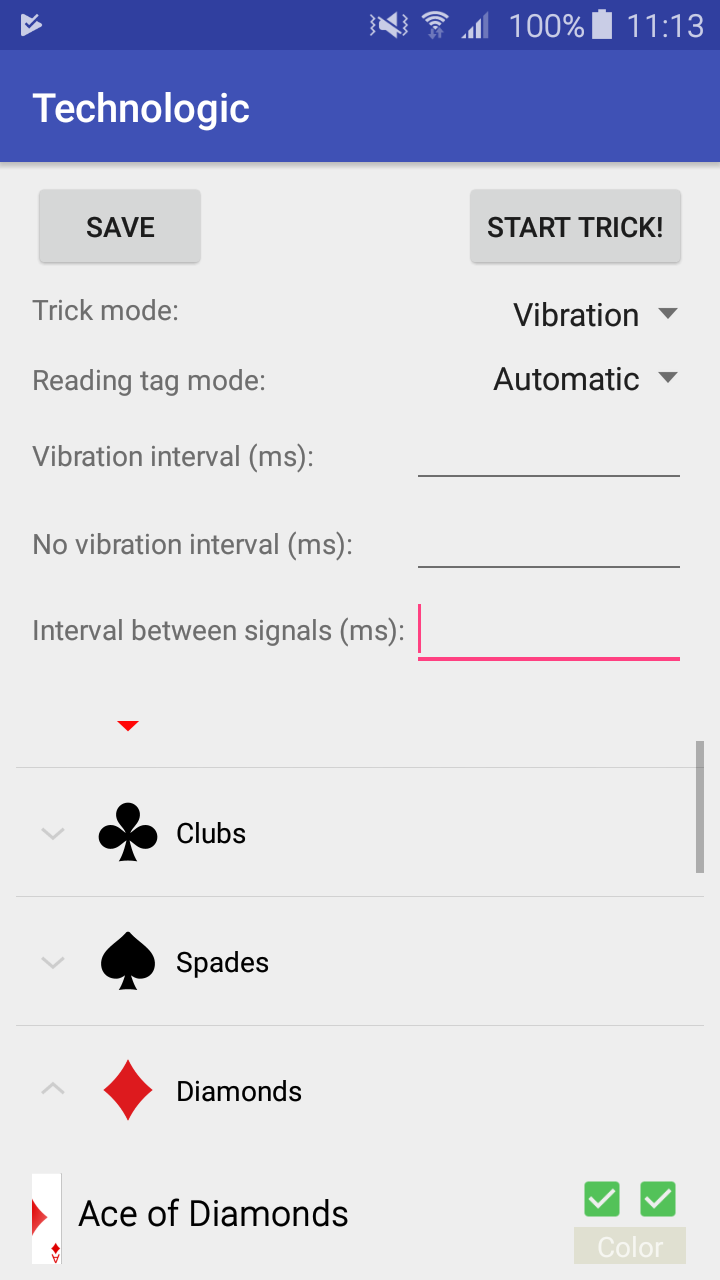
\includegraphics[scale=0.22]{imgs/mainActivity.png}
\caption{Panel konfiguracyjny aplikacji}
\end{figure}
Przycisk \textit{START TRICK!} uruchamia Aktywność określoną w opcji \textit{Trick mode}. Dostepne są trzy możliwości: tryb zapisywania wartości do znaczników oraz dwa rodzaje odczytywania (Fotografia lub Wibracje). Opcja \textit{Reading tag mode} ma dwie możliwości do wyboru, automatyczny lub manualny. Odpowiada to za operacje związane z NFC, mogą się one wykonywać automatycznie po wykryciu tagu lub na żądanie poprzez wciśnięcie przycisku. \textit{Vibration interval} odpowiada za długość (w milisekundach) trwania pojedynczej wibracji. \textit{No vibration interval} to długość (w milisekundach) odstępu między dwoma wibracjami, gdy sygnalizujemy wartość 0. \textit{Interval between signals} to długość (w milisekundach) trwania przerwy między sygnalizowanymi bitami. Każda z grup koloru kart ma elementy, które zawierają informacje na temat nazwy oraz schematu wibracji kolejnych kart. Nazwę karty podajemy w polu tekstowym znajdującym się po prawej stronie od ikony reprezentującą tę kartę, natomiast schemat wibracji ustalamy za pomocą pól wyboru. Dla ułatwienia mają one podpis, które z nich odpowiadają za kolor, a które za wartość karty. Przycisk \textit{SAVE} służy do zapisania ustawień do pliku, dzięki czemu będą one się automatycznie ładować przy starcie aplikacji. 
\par
Po przygotowaniu wszelkich niezbędnych elementów, możemy przystąpić do wykonywania triku. Smartfona z aplikacją chowamy do kieszeni. Aplikacja musi być na pierwszym planie i urządzenie nie może być zablokowane. Zaleca się skorzystanie z pokrowca, aby aplikacja przez przypadek nie przeniosła się na inny plan. Wybieramy widza z publiczności, podajemu mu talię i prosimy go o przetasowanie kart. Następnie prosimy go o wybranie dowolonej karty z talii, zapamiętaniu jej i umieszczeniu w woreczku. Odbieramy od niego resztę talii, a woreczek wkładamy dyskretnie do kieszeni (w tym momencie aplikacja odczytuje zawartość ze znacznika). Dalszy przebieg występu zależy od wybranego wcześniej wariantu. Kluczowym działaniem dla obu wariantów jest dezorientacja czasowa w postaci historyjki.
\paragraph{Fotografia}\mbox{}\\


% \noindent\textbf{\large{Fotografia}}\par
Możemy odłożyć karty, nie będą potrzebne. Ten wariant można zakończyć na dwa sposoby. W zależności od wybranego zakończenia będzie zastosowana inna historyjka. \par 
Pierwszą opcją jest zrobienie zdjęcia portretowego widzowi za pomocą aplikacji. Na fotografii zostanie umieszczony obrazek ze wzorem karty widza na wysokości jego czoła. Historyjką dla tego zakończenia mogłoby być: "W dzisiejszych czasach technologia coraz bardziej ingeruje w ludzki umysł. Nie orientujemy się kiedy urzędzenia czytają nam w myślach upraszczając nam codzienne życie. O ilu rzeczach nie musimy pamiętać, ponieważ coś robi to za nas. Mój smartfon również posiada taką możliwość. On umie czytać w myślach! Nie wierzycie? Pozwólcie, że zaprezentuję (...)"\par
Drugą opcją jest podanie widzowi pytajnika. Następnie robimy dowolne zdjęcie widzowi, w taki sposób, aby pytajnik był widoczny. Na fotografii, obraz pytajnika zostanie zastąpiony obrazem ze wzorem karty widza. W tym przypadku historyjką mogłoby być: "Teraz drodzy Państwo chciałbym Wam przedstawić magiczną kartę. Jest bardzo skryta, a swoją wartość trzyma wewnątrz siebie i nieczęsto ukazuje ją światu. Jednakże jest bardzo podatna na sławę, wtedy ujawnia swoją tajemnicę. Spróbujmy nagrodzić ją brawami, a Pan/Pani niech jej powie, że jest jej największym fanem i zapozuje z nią do zdjęcia. Będę paparazzi! (...)"\par
W obu sytacjach efektem triku jest fotografia, na której widnieje karta widza. Można ją wysłać widzowi na pamiątkę, gdyż znajduje się ona w pamięci smartfonu w folderze Technologic.
\paragraph{Wibracje}\mbox{}\\
Ten wariant jest trudniejszy i wymaga pewnych umiejętności od magika. Talię można zostawić przy sobie, gdyż może się przydać do odgadywania karty. Po umieszczeniu woreczka z kartą w kieszeni, smartfon zacznie wibrować przekazując konkretny schemat wibracji ustalony wcześniej w aplikacji. Dzięki znajomości schematu, jesteśmy w stanie wywnioskować jaką kartę wybrał widz. Historyjką do tego zakończenia mogłoby być: "Wielu magików odnajduje wybrane karty w różnych miejscach, które wydają się niemożliwe. Ja natomiast odnajdę kartę w miejscu gdzie jej nie ma! Będę wykładać odkryte karty na stół i na ich podstawię powiem jakiej karty brakuje w talii!". Podczas wykładania kart, nie należy grupować kart w jeden stosik. Niech z kart ułoży się wzór  odpowiadający wartości karty znajdującej się w kieszeni. To sprawi wrażenie, że od momentu wykładania kart na stół wiedziałeś jakiej karty brakuje.\par
Po zakończeniu triku w pierwszym wariancie nie należy chować telefonu do kieszeni z woreczkiem. Najlepiej odłożyć go gdzieś lub ewentualnie schować do innej kieszeni. W drugim wariancie natomiast nie należy wyciągać telefonu z kieszeni, aby uniknąć podejrzeń.
 \newpage
\section{Platforma Android}
Android to system operacyjny przeznaczony dla urządzeń mobilnych z jądrem Linuxa. Jego kolejne wersje zaczynają się na kolejne litery alfabetu i nawiązują do jakieś słodkiej przekąski lub deseru. Trzema najpopularniejszymi wersjami na rynku są Lollipop, Marshmallow i Nougat. Ostatnią wypuszczoną wersją jest Oreo (sytuacja z grudnia 2017). Każda z wersji udostępnia własny interfejs programowania aplikacji (ang. application programming interface) zwany \textbf{API}. Im nowsza wersja, tym wyższy jest poziom API, który daje nam szersze możliwości programistyczne.
\subsection{Programowanie obiektowe}
Podejście do sposobu programowania zmieniało się w czasie. Tradycyjnym podejściem było programowanie proceduralne. Polegało ono na rozdzieleniu danych od operujących na nich funkcji. Niestety takie podejście odizolowania danych od kodu może spowodować przypadkową ich modyfikację przez procedury, które nie były logicznie z nimi związane. Do takiego programu ciężko również było wprowadzić wszelkie modyfikacje. \par
Na początku lat 60. XX w. pojawiła się pierwotna koncepcja programowania obiektowego. Miała ona być bardziej naturalna dla ludzkiego mózgu, a samo programowanie stać się bardziej zgodne z rzeczywistością. Popularność zdobyła dopiero w okolicach lat 80. XX w., gdy pojawił się język C++ rozszerzający język C. Wyniknęło to ze wzrostu popularności graficznych interfejsów użytkownika, do których koncepcja programowania obiektowego sprawdza się wzorowo.\par Tworzenie programu zgodnego z koncepcją programowania obiektowego sprowadza się do rozdzielenia logiki na osobne klasy (typy danych), istniejące w tych klasach procedury oraz trzymaniu się konkretnych zasad. Te zasady nazywamy \textbf{paradygmatami programowania obiektowego}.
\paragraph{Abstrakcja (ang. abstraction)}\mbox{}\\ Sprowadzenie danego problemu do prostszej postaci. Polega na wyznaczeniu dla obiektów cech, niezbędnych dla algorytmów, ale jednocześnie niezależnych od implementacji.
\paragraph{Enkapsulacja (ang. encapsulation)}\mbox{}\\ Ukrycie cech obiektu. Zewnętrzne otoczenie nie może zmienić danych znajdujących się wewnątrz obiektu w nieoczekiwany sposób. Każda klasa udostępnia abstrakcyjną reprezentację siebie zwaną interfejsem. Za jego pomocą zewnętrzne otoczenie może się komunikować z danym obiektem.
\paragraph{Polimorfizm (ang. polymorphism)}\mbox{}\\ Używanie wartości zmiennych i podprogramów na kilka różnych sposobów. Wykazywanie przez metodę różnych form działania w zależności od tego jaki typ obiektu jest wskazywany przez wskaźnik lub referencję.
\paragraph{Dziedziczenie (ang. inheritance)}\mbox{}\\ Porządkuje polimorfizm i enkapsulację przez definiowanie i tworzenie specjalizowanych obiektów na podstawie bardziej ogólnych.

\paragraph{Obiekt a klasa}\mbox{}\\
Podstawową cegiełką każdego programu zgodnego z koncepcją programowania obiektowego jest obiekt. Obiekt to nie to samo co klasa. Klasa opisuje pola (zmienne) i metody (procedury) dla wszystkich reprezentantów tej klasy, czyli obiektów.\par Zarówno pola jak i metody muszą mieć określony poziom dostępu. Wyróżniamy trzy poziomy dostępu: publiczny, chroniony oraz prywatny. Dostęp publiczny oznacza, że dany atrybut może zostać użyty zarówno w obiekcie tej klasy jak i poza nim. Dostęp chroniony pozwala na używanie atrybutów tylko w obiekcie tej klasy, ale również w obiektach dziedziczących z tej klasy. Dostęp prywatny nie zezwala na używanie atrybutów klasy żadnym obiektom nie będącymi reprezentacją tej klasy. Jeśli nie podamy jawnie poziomu dostępu do danego atrybutu, zostanie on potraktowany jako prywatny, jest to domyślny poziom dostępu.\par Wszystkie pola klasy powinny mieć dostęp prywatny, a modyfikację tych pól powinny być ewentualnie możliwe przez publiczne metody wykonujące operacje na tych polach. Metodę publiczną pobierająca wartość danego pola nazywamy getter'em, natomiast metodę ustawiającą wartość danemu polu setter'em.\par Każdy z atrybutów może być dodatkowo statyczne dla danej klasy. Oznacza to, że możemy odwołać się do tego atrybutu bez tworzenia reprezentanta tej klasy. Najczęściej takie statyczne atrybuty mają dostęp publiczny. Jeśli metoda nie jest zadeklarowana jako statyczna, może zostać zadeklarowana jako wirtualna. Oznacza to, że nie można wywołać tej metody dopóki nie zostanie ona nadpisana w klasie dziedziczącej.\par Klasa implementuje tylko abstrakcyjny typ danych więc pamięć przydzielana jest dopiero do obiektów, a nie do samej klasy. Natomiast obiekt jest już strukturą zawierającą dane oraz funkcje pracujące na tych danych. Każdy obiekt będący reprezentantem danej klasy nazywamy instancją tej klasy. Każda instancja ma taki sam zestaw pól oraz metod, jednakże mogą się różnić wartościami pól wewnątrz. Tworzenie instancji następuje przez wywołanie konstruktora. Konstruktor to specjalna metoda w klasie, musi mieć ona identyczną nazwę co klasa. Po wywołaniu konstruktora następuje alokacja pamięci dla obiektu, połączenie tego obszaru z metadanymi z klasy, wykonaniu kodu klasy bazowej oraz konstruktora. Dopiero wtedy nasz obiekt zaczyna fizycznie istnieć. Jednakże zmienna obiektowa nie przechowuje wewnątrz siebie danych obiektu, ona przechowuje referencję do tego obiektu. Referencja to wartość, która informuje o lokalizacji danych obiektu w pamięci.\par Istnieją klasy, których instancji nie można utworzyć. Nazywamy je klasami abstrakcyjnymi. Klasa abstrakcyjna musi posiadać conajmniej jedną metodę wirtualną w sobie. Jeśli posiada wyłącznie metody wirtualne, jest wówczas nazywana interfejsem klasy.


\subsection{Programowanie na Androida}
Android nie ma ściśle określonej technologii, za pomocą której można tworzyć dla niego aplikacje. Wybór zależy od efektów jakie chcemy osiągnąć. Technologii za pomocą, których chcielibyśmy tworzyć aplikację jest bardzo dużo, jednakże można je podzielić na dwa rodzaje. Programowanie natywne (np. Android oraz JNI) zwięszy wydajność aplikacji. Programowanie multiplatformowe (np. Apache Cordova oraz Xamarin) zwiększy przenośność. 
\paragraph{Android-Java}\mbox{}\\
Jest najpopularniejszą technologią do tworzenia aplikacji na Androida. Jak nazwa wskazuje, bazuje ona na języku Java, chociaż często nazywa się tę technologię po prostu Android. Programista ma dostęp do obszernej dokumentacji całego języka.
\paragraph{Java Native Interface (JNI)}\mbox{}\\
Java Native Interface jest to framework, który umożliwia aplikacji Java uruchomionej na wirtualnej maszynie Javy (ang. Java Virtual Machine) wołać funkcje natywne. To znaczy takie, które wykonują się bezpośrednio na komponentach komputera, napisane w innych językach programowania takich jak C czy C++. Możliwe jest także wołanie metod kodu Java przez natywne aplikacje. Możliwe jest użycie tego interfejsu na platformie Android. Kod natyny wykonuje się znacznie szybciej w porównaniu do Javy. Kolejną powodem do stosowania JNI jest fakt, że istnieje wiele bibliotek i narzędzi w językach C i C++, które nie mają swoich odpowiedników dla języka Java. Wywołanie metody natywnej z poziomu kodu Javy jest kosztowne. Pojedyncze wywołanie takiej metody trwa znacznie dłużej niż zawołanie takiej metody w obrebie jednej platformy. Dodatkowo tablice często są kopiowane dla funkcji natywnej, a po jej wykonaniu kopiowane są z powrotem dla kodu Java. Przykładowy kod z wykorzystaniem JNI w środowisku Android, zwracający łańcuch znaków: 
\begin{lstlisting}[language=C]
#include <jni.h>
#include <string>

extern "C"
JNIEXPORT jstring JNICALL
Java_com_example_maciej_myapplication_MainActivity_stringFromJNI(
        JNIEnv *env,
        jobject /* this */) {
    std::string hello = "Hello from C++";
    return env->NewStringUTF(hello.c_str());
}
\end{lstlisting}

Dodatkowo w kodzie Java potrzebna jest deklaracja funkcji
\begin{lstlisting}[language=C]
public native String stringFromJNI();
\end{lstlisting}
\paragraph{Apache Cordova}\mbox{}\\
Cordova to framework, który opakowuje aplikację HTML/JavaScript do macierzystego kontenera, który ma dostęp do funkcji urządzenia na kilku platformach. Funkcje te są udostępniane za pośrednictwem zunifikowanego interfejsu JavaScript API, dzięki czemu można łatwo napisać jeden zestaw kodu.
\paragraph{Xamarin}\mbox{}\\
Xamarin jest platformą, na której w język C\# jesteśmy w stanie stworzyć aplikacje na Androida, WindowsPhona i iOS jednocześnie. Posiada specjalne zestawy narzędzi dla programistów (ang. software development kit) zwane SDK: Xamarin.iOS i Xamarin.Android. Tworzenie na WindowsPhona nie wymaga dodatkowego SDK.
\subsection{Intencja}
\textbf{Intencja (ang. Intent)} to abstrakcyjny opis akcji jaką chcemy wykonać. Możliwości wykonania akcji przy pomocy Intencji jest bardzo dużo. Do podstawowych zalicza się przejście do kolejnego widoku w aplikacji czy wykonanie zdjęcia. Pełni ona rolę spoiwa między kodem różnych aplikacji. Opisuje ona czynność do wykonania, dzięki czemu osobna aplikacja realizuje swoją pracę i odsyła ewentualne wyniki. Pierwszorzędnymi atrybutami struktury Intencji jest opis akcji do wykonania oraz ewentualne dane niezbędne do wykonania tej akcji. Do drugorzędnych atrybutów należą:
\begin{itemize}
\item Kategoria (ang. category) - zapewnia dodatkową informację na temat akcji do wykonania.
\item Typ (ang. type) - precyzuje typ danych jaki jest przekazywany.
\item Komponent (ang. component) - precyzuje nazwę komponentu (klasy), która będzie używała Intencji. Zazwyczaj jest to określone z pozostałych atrybutów i na podstawie tego dopasowywany jest komponent, który obsłuży daną akcję. Ustalenie tego atrybutu powoduje, że pozostałe są opcjonalne.
\item Dodatki (ang. extras) - przechowuje wszelkie dodatkowe informacje jakie chcielibyśmy przekazać do komponentu.
\end{itemize}
Ponadto każdej Intencji możemy ustawić flagi. Lista dostępnych flag jest opisana w dokumentacji Androida. Zapewniają one dodatkowe informacje konfiguracyjne np. ustawienie flagi \textit{FLAG\_FROM\_BACKGROUND} informuje, że dana Intencja pochodzi od procesu w tle, a nie od interakcji użytkownika.
Istnieją dwie podstawowe formy Intencji:
\begin{itemize}
    \item Jawne (ang. explicit) Intencje mają określony atrybut komponent. Można tego dokonać poprzez metodę \textit{setComponent()} lub \textit{setClass()}. Dzięki temu, jednoznacznie jest ustalona klasa, która ma zająć się wykonaniem akcji określonej w Intencji.
    \item Niejawne (ang. implicit) Intencje nie określają atrybutu komponent. Muszą natomiast, poprzez pozostałe atrybuty, zawierać wystarczająco dużo informacji, aby system określił, który z dostępnych komponentów będzie najlepszy do przeprowadzenia danej akcji.
\end{itemize}
Rozstrzygnięcie niejawnej Intencji następuje na podstawie trzech atrybutów: akcji, typu i kategorii. Korzystając z tych informacji wykonywane jest zapytanie w menadżerze pakietów dla komponentu, który może obsłużyć Intencję. Decyzję o tym czy dany komponent zostanie użyty określa się w następujący sposób. Jeśli został ustalony atrybut akcja i/lub typ w Intencji, to musi on być również wymieniony przez komponent jako obsługiwany.  Natomiast określenie kategorii odnosi się do Aktywności, musi ona obsługiwać daną kategorię, aby zrealizować Intecję.\cite{intent}
\subsection{Manifest}
Każda aplikacja w technlogii Android musi posiadać plik AndroidManifest.xml w swoim głównym folderze. Zapewnia nazwę pakietu Java dla aplikacji, która pełni rolę unikalnego identyfikatora. Manifest dostarcza podstawowych informacji o aplikacji (etykieta, ikona) do systemu Android, które musi posiadać, zanim będzie mógł uruchomić kod aplikacji.  Zawiera listę bibliotek, z którymi aplikacja musi być połączona. Opisuje komponenty aplikacji oraz podaje nazwy klas ich implementujących. Deklaruje minimalny poziom interfejsu API Androida oraz uprawnienia, które muszą być spełnione do prawidłowego funkcjonowania. Zgoda użytkownika co do uprawnień jest niezbędna, aby aplikacja mogła korzystać z chronionych części API. Niezbędnym elementem do ustawienia jest ustalenie widoku, który się wyświetli przy pierwszym uruchomieniu. Dokonuje się tego poprzez Filtr Intencji (ang. Intent Filter). Wystarczy w elemencie opisującym Aktywność wstawić Filtr Intencji z odpowiednimi wartościami atrybutów akcji oraz kategorii (odpowiednio \textit{android.intent.action.MAIN} oraz \textit{android.intent.category.LAUNCHER}).\cite{manifest}
\subsection{Zasoby}
W dzisiejszych czasach często wprowadza się zmiany w istniejących aplikacjach. Może to być spowodowane zmianą właściciela aplikacji, decyzją ulepszenia aplikacji lub po prostu ludzkim kaprysem. Dlatego wysoki nacisk kładzie się na to, aby aplikacja była łatwo modyfikowalna. Android zapewnia mechanizm określonym jako \textbf{Zasoby (ang. Resources)}.\par Wszelkie Zasoby powinny zostać podzielone i umieszczone w specjalnych podfolderach katalogu z zasobami o nazwie \textit{/res}. Mamy kilka takich specjalnych podfolderów do wyboru, między innymi folder \textit{/drawable} służy do przechowywania w nim obrazków wyświetlanych w aplikacji. Folder \textit{/color} zawiera zdefiniowane kolory używane w aplikacji. Folder \textit{/layout} zawiera pliki xml opisujące widoki używane w komponentach graficznych aplikacji. Folder \textit{/values} przechowuje kilka plików xml zawierających proste wartości takie jak łańcuchy znaków \textit{(/strings.xml)} lub wartości liczbowe np. \textit{/dimens.xml}.\cite{providing_resources}\par Kiedy aplikacja zostaje skompilowana, zostaje wygenerowana klasa R. Zawiera ona identyfikatory wszystkich zasobów umieszczonych w podfolderach \textit{/res}. Dla każdego podfolderu katalogu \textit{/res} istnieje podklasa w klasie R. Przykładowo dla obrazka \textit{hello.png} znajdującego się w podfolderze \textit{/drawable} mamy podklasę w postaci R.drawable, w której znajduje się statyczne pole hello, możemy się do niego odwołać poprzez R.drawable.hello. Dzięki temu uzyskujemy identyfikator danego zasobu, który jest liczbą całkowitą. Wiele obiektów w Androidzie ma metody, które przyjmują jako parametr identyfikator zasobu.\cite{accessing_resources}

\subsection{Aktywność}
\textbf{Aktywność (ang. Activity)} służy głównie do interakcji z użytkownikiem. Z tego względu klasa ta odpowiedzialna jest za utworzenia okna gdzie umieszczane są komponenty interfejsu użytkownika. Najczęściej jej zawartość przedstawia się na pełnym ekranie. Jednakże może również zostać użyta jako ruchome okno lub jako wbudowany element innej Aktywności tworząc większy komponent. Nowa klasa Aktywności musi dziedziczyć po klasie bazowej AppCompatActivity oraz w projekcie musi się również znajdować przygotowany dla niej zasób zawierający jej widok. Możemy wówczas nadpisać każdą z dostępnych metod z klasy bazowej, dodawać własne pola oraz pisać własne metody. Najważniejszą metodą do nadpisania jest onCreate(Bundle). Należy w niej wywołać analogiczną metodę rodzica oraz ustawić dla tej aktywności odpowiedni widok za pomocą metody setContentView(int). Metoda setContentView(int) przyjmuje jako parametr identyfikator zasobu zawierającego informacje o widoku danej aktywności.\cite{activity} Przykład:
\begin{lstlisting}[language=Java]
public class MainActivity extends AppCompatActivity {
    @Override
    protected void onCreate(Bundle savedInstanceState) {
        super.onCreate(savedInstanceState);
        setContentView(R.layout.activity_main);
    }
}
\end{lstlisting}
W tym przykładzie nasza aktywność jest absolutnie pusta. Użytkownik widzi jedynie biały ekran, z którym nie ma żadnej interakcji. Bez dodatkowych komponentów graficznych niewiele uda się tu osiągnąć. Jednakże są pewne elementy, które mogą zapewnić interakcję z użytkownikiem poprzez samą pustą Aktywność. Jednym z nich jest obiekt \textbf{Toast (ang. Toast)}.\par Jest to widok, który zawiera krótką wiadomość dla użytkownika. Jest ona wyświetlana na ekranie przez krótką chwilę, po czym automatycznie znika. Pozycję można dowolnie ustalić, domyślnie wyświetla się u dołu ekranu. Ten element jest nieresponsywny, aby uniknąć wprowadzenia użytkownika w błąd. Ideą tego mechanizmu jest, aby powiadomić dyskretnie użytkownika o jakieś sytuacji np. jego ustawienia zostały zapisane. Najprościej wykorzystać tę klasę poprzez wywołanie jednej ze statycznych metod, która ustawi wszystko czego potrzebujemy i zwróci nam obiekt klasy Toast. Jedną z tych metod jest \textit{makeText(Context context, CharSequence text, int duration)}. Parametr \textit{context} to kontekst aplikacji. Jest globalną informacją o stanie środowiska. Innymi słowy, gdy tworzymy nowy obiekt nierzadko musi on wiedzieć co się w danym momencie dzieje w aplikacji, aby funkcjonował prawidłowo. Najczęściej podajemy tam po prostu kontekst Aktywności, w której aktualnie się znajdujemy. Parametr \textit{text} jest niczym innym jak łańcuchem znaków, który zostanie wyświetlony w Toaście. Alternatywnie możemy podać w to miejsce zasób, który zawiera łańcuch znaków. Ostatni parametr \textit{duration} jest określeniem jak długo ma się wyświetlać ta informacja. Należy tutaj podać jedną z dwóch stałych znajdujących się w klasie Toast, LENGH\_SHORT lub LENGHT\_LONG. Po wywołaniu tej metody zostanie nam zwrócony obiekt typu Toast, aby wyświetlić jego zawartość na ekranie należy wywołać na końcu metodę \textit{show()}.\cite{toast} Przykład:
\begin{lstlisting}[language=Java]
Toast.makeText(this, "Hello World!", Toast.LENGHT_SHORT).show();
\end{lstlisting}\par
Odwoływanie się do poszczególnych elementów z pliku zawierającego widok Aktywności następuje poprzez metodę \textit{findViewById(int id)}. Parametr \textit{id} to identyfkator elementu interfejsu, który znajduje się na widoku. Nie musimy pamiętać lub zapisywać tych identyfikatorów. Mamy do nich dostęp poprzez klasę \textit{R.id}, która zawiera w sobie wszystkie identyfikatory. Obiekt zwracany przez metodę \textit{findViewById(int id)} należy zrzutować na odpowiedni typ. \begin{lstlisting}[language=Java]
private void initializeSpinners(){
Spinner trickModeSpinner = (Spinner)findViewById(R.id.trickModeSpinner);
}
\end{lstlisting}
\par
Podczas pracy na Androidzie możemy minimalizować aplikację, wyłączać ją, blokować ekran, przechodzić między kolejnymi widokami. Każda z tych sytuacji wpływa na Aktywności, które były uruchomione. Poniższy schemat przedstawia cykl życia Aktywności, przy niektórych działaniach ze strony użytkownika lub systemu. Na końcu każdej strzałki znajduje się nazwa metody jaka jest wywoływana w aktywności na rzecz, której wydarzyła się dana akcja.
\begin{figure}[H]
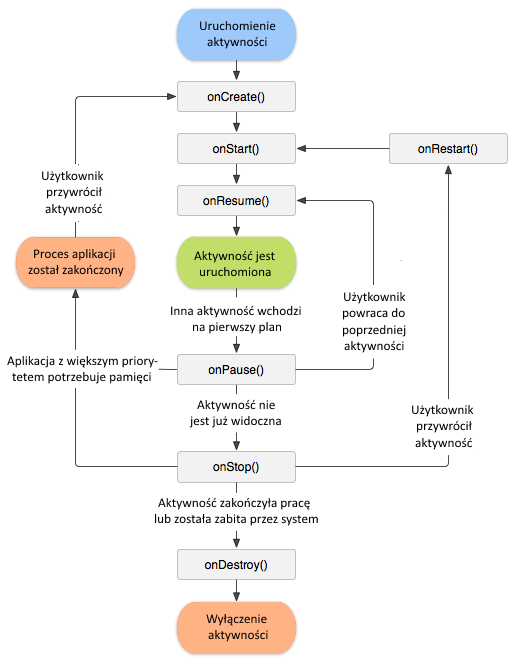
\includegraphics[scale=0.9]{imgs/activity_lifecycle_pl.png}
\caption{Cykl życia aktywności\cite{activity}}
\end{figure}

\subsection{Warstwa ograniczeń}
O Aktywności można myśleć jak o sztaludze. Jest to dopiero podstawa dla dalszej pracy. Aby namalować obraz, będzie nam potrzebne płótno. Analogicznie, aby wyświetlić coś na ekranie, będzie nam do tego potrzebna warstwa. Jest to podstawowy element interfejsu użytkownika, na którym możemy budować kolejne komponenty lub bardziej skomplikowane struktury.\par\textbf{Warstwa ograniczeń (ang. contraint layout)} to specjalna warstwa, która pozwala na pozycjonowanie komponentów oraz określenie ich wymiarów w bardzo elastyczny sposób. Dokonuje się tego za pomocą \textbf{Ograniczeń (ang. constraints)}.\par Są one relacją między komponentami. Informują o tym gdzie i w jakiej odległości leżą od siebie elementy widoku. Dzięki nim można budować interfejs na kilka sposobów. Rozmiar możemy ustawić poprzez rozciąganie lub zwężanie w dowolnych kierunkach komponentu. Wówczas mówi się, że ten element ma ustalony (ang. fixed) rozmiar. Alternatywą dla określenia wymiarów komponentu jest ustawienie, aby ograniczył się on do rozmiaru jaki zajmuje jego zawartość (ang. wrap-content). Jeśli chcemy ustalić szerokość lub wysokość, można tego dokonać za pomocą jednej z opcji: dopasuj do rodzica (ang. match-parent) lub dopasuj do ograniczeń (ang. match-constraint). Dopasowanie do rodzica spowoduje wpasowanie komponentu wertykalnie lub horyzontalnie do zewnętrznych krawędzi rodzica. Dopasowanie do ograniczeń ustali rozmiar elementu na podstawie określonych dla niego ograniczeń horyzontalnych lub wertykalnych. Jednakże należy mieć na uwadze, że bazowa klasa komponentu może nie być przystosowana do zmiany rozmiarów (np. nie posiada algorytmu skalującego domyślnej grafiki). Pozycję kolejnych elementów możemy uzależniać od pozycji już umieszczonych widoków.\par \textbf{Pozycjonowanie relatywne (ang. relative positioning)} jest najprostszym sposobem pozycjonowania. Kolejny element interfejsu użytkownika ustawiany jest wybraną krawędzią do wybranej krawędzi rodzica. 
\begin{figure}[H]
\centering
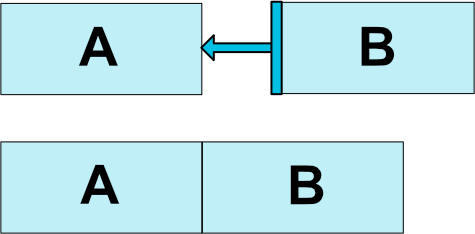
\includegraphics[scale=0.7]{imgs/relative-positioning.png}
\caption{Przykład relatywnego pozycjonowania\cite{constraintlayout}}
\end{figure} Można rozszerzyć ten mechanizm o dodatkowe marginesy. Wówczas możemy wprowadzić atrybut z wartością liczbową mówiącą o tym o ile od siebie mają być oddalone ustalone wcześniej krawędzie. \cite{constraintlayout}
\subsubsection{Elementu graficzne interfejsu}
Na utworzonej wcześniej warstie ograniczeń możemy umieszczać wybrane przez nas komponenty interfejsu graficznego. Dla każdego z komponentów ustalamy ich rozmiar oraz położenie na warstwie ograniczeń.
\paragraph{Etykieta (ang. Text View)}\mbox{}\\
Wyświetla na danym obszarze zwyły tekst. Służy głównie do przekazywania informacji. Brak interakcji z użytkownikiem.\cite{textview}
\paragraph{Przycisk (ang. Button)}\mbox{}\\
Najprostszy interaktywny element, użytkownik może w niego kliknąć co spowoduje wywołanie metody \textit{onClick()} w obiekcie Przycisku. \cite{button}
\paragraph{Przycisk wyboru (ang. Check Box)}\mbox{}\\
Ma bardzo podobne działanie do przycisku, jednakże różni się od niego tym, że posiada stan \textit{prawdy} lub \textit{fałszu}. Akcję po zmianie stanu przycisku wyboru można przeprowadzić poprzez nadpisanie metody \textit{onCheckChanged()}.
\paragraph{Pole tekstowe (ang. Edit Text)}\mbox{}\\
Kolejny prosty interaktywny element, użytkownik po kliknięciu w to pole może wprowadzić jakąś wartość. Może to być wartość liczbowa, słowna lub inna ustalona przez programistę. Służy głównie do uzyskiwania danych od użytkownika. Istnieje opcja ustawienia reagenta na zmiany wartości tego pola, jest to obiekt klasy Obserwatora Tekstu (ang. Text Watcher).\cite{edittext}
\paragraph{Lista rozwijana (ang. Spinner) i Widok listy rozszerzanej (ang. Expandable List View)}\mbox{}\\
Wyświetla opcje w postaci listy. Dla tych kontrolek niezbędne jest stworzenie dwóch dodatkowych obiektów. Adaptera, czyli obiektu zawierającego dane do wyświetlenia w odpowiednim formacie. Reagenta na wybranie pozycji z listy (ang. On Item Click Listener) i odpowiednim nadpisaniu mu metody \textit{onItemClick(AdapterView parent, View view, int position, long id)}.\cite{adapterview}
\subsection{Singleton}
Zdarza się, że w ramach naszej aplikacji chcielibyśmy posiadać globalny obiekt zawierający zestaw pól i metod, z których chcielibyśmy korzystać. Problem w tym, że każdy nowo utworzony obiekt, ma bazowe parametry, a my chcielibyśmy obiekt, który raz zmieniony zapamiętuje swoją zmianę przy kolejnych dostępach. W takiej sytuacji tworzymy właśnie Singleton, niestety nie ma dobrego polskiego tłumaczenia. Realizuje się to poprzez utworzenie w tej klasie statycznego pola, które jest obiektem tej klasy oraz statycznej metody zwracającej właśnie to pole. Oto nasza realizacja:
\begin{lstlisting}[language=Java]
public class SettingsSingleton {
    private static SettingsSingleton ourInstance = new SettingsSingleton();
    
    private SettingsSingleton(){};
    
    public static SettingsSingleton getInstance(){
        return ourInstance;
    }
}
\end{lstlisting}
Dzięki takiemu rozwiązaniu w dowolnym miejscu w kodzie możemy dostać się do obiektu \textit{SettingsSingleton} poprzez \textit{SettingsSingleton.getInstance()}. Wszelkie modyfikacje wprowadzone w tym obiekcie będą aktualne przy każdym dostępie do tego obiektu.
\subsection{System plików}
Jako użytkownik, na urządzeniu mobilnym z systemem operacyjnym Android, mamy swobodny dostęp do systemu plików poprzez interfejs graficzny. Możemy dostać się do plików dowolnej aplikacji. Jako programista również mamy dostęp do systemu plików. Możemy utworzyć folder aplikacji w pamięci urządzenia i przechowywać w nim wszelkie niezbędne dane do jej prawidłowego funkcjonowania. Dostęp do głównego katalogu pamięci urządzenia realizuje się przy pomocy klasy \textit{File}, która reprezentuje zarówno pliki jak i katalogi (zgodnie z filozofią systemu Linux). Podajemy jej w konstruktorze ścieżkę do tego folderu, można ją uzyskać poprzez statyczną metodę w klasie Środowiska (ang. Environment) -  \textit{Environment.getExternalStorageDirectory()}. Gdy mamy uchwyt do tego katalogu możemy w nim dowolnie tworzyć nowe katalogi metodą \textit{mkdirs()} lub pliki metodą \textit{createNewFile()}.
\subsection{Wibrator}
Wibrowanie urządzenia możliwe jest przy użyciu klasy Wibrator (ang. Vibrator). Obiekt tej klasy uzyskuje się poprzez wywołanie metody klasy Kontekst (ang. Context) \textit{getSystemService(Context context)}. Jako parametr \textit{context} należy podać stałą \textit{Context.VIBRATOR\_SERVICE}. Należy pamiętać, aby wynik tej metody zrzutować na klasę Wibratora.\par Najprostszym użyciem tej klasy jest wywołanie metody \textit{vibrate(long miliseconds)}, która spowoduje, że urządzenie będzie wibrowało przez podany okres. Istnieje możliwość stworzenia bardziej skomplikowanego schematu wibracji dzięki metodzie vibrate (long[] pattern, int repeat). Paremetr \textit{pattern} to tablica, której elementy stojące na nieparzystych pozycjach są okresami wibrowania, a parzyste elementy to okresy przerwy między wibracjami. Parametr \textit{repeat} informuje o tym ile razy podana sekwencja ma zostać powtórzona. Jeśli chcemy podany schemat wykonać tylko raz, należy podać w tym parametrze wartość -1. Wibrator udostępnia możliwość odgrywania efektów dźwiękowych podczas wibracji. Jeśli wyjdziemy z aktywności, która odpowiada za wibracje, nie będą one kontynuowane.\cite{vibrator}
\subsection{Aparat}

Możliwe jest użycie wbudowanego aparatu poprzez wbudowaną systemową aplikację. Wywołuje się ją przy użyciu intencji. Atrybutem określającym rodzaj akcji jest tutaj MediaStore.ACTION\_IMAGE\_CAPTURE podany jako parametr konstruktora intencji. Po utworzeniu intencji w jej dodatkach należy umieścić ścieżkę w jakiej ma być zapisane wykonane zdjęcie. W celu uruchomienia aparatu w bieżącym kontekście wołamy metodę startActivityForResult. W parametrach tej metody umieszczamy intencję oraz kod identyfikujący te wywołanie przy powrocie. Po zakończeniu działania aparatu w funkcji onActivityResult sprawdza się kod identyfikujący uruchomioną aktywność. Jeśli kod zgadza się z tym który umieściliśmy w wywołaniu aparatu, możemy wywołać akcje które powinny się wykonać zaraz po wykonaniu zdjęcie np zaktualizowanie widoku.
 \newpage
\section{Kaskadowe klasyfikatory cech Haar'a (Maciej Plewka)}

Wybraną metodą zaimplementowaną w celu zrealizowania wariantu sztuczki z fotografią, w którym potrzebne jest wskazanie obiektu na zdjęciu, są kaskady Haar'a. Jest to bardzo skuteczny i szybki sposób detekcji oparty na kaskadowych klasyfikatorach cech. Metoda ta działa sprawnie przetwarzając wideo w czasie rzeczywistym, więc w doskonale sprawdza się w naszym przypadku, ze względu na szybki czas działania. Takie rozwiązanie detekcji obiektów zostało zaprezentowane przez Paula Viola i Michael Jones w jednej z ich prac naukowych \cite{violaJones}.

\subsection{Cechy Haar'a}
Proces detekcji obiektów oparty jest o tzw. Cechy Haara. Są to prostokąty takie jak przedstawiono na rysunku \ref{fig:cechyHaara}. Zawierają one informacje na temat różnicy wartości pikseli na zaznaczonych obszarach, dodatkowo wartości te są przeskalowane odwrotnie porcjonalnie do ich wielkości.
\begin{figure}[H]
	\centering
	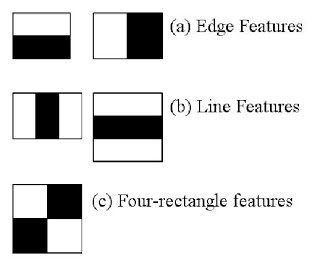
\includegraphics[scale=0.5]{imgs/cechy.jpg}
	\caption{{Cechy Haara Źródło:} \cite{faceDetectionOpenCV}}
	\label{fig:cechyHaara}
\end{figure}

Zdefiniowane zostały 3 rodzaje cech. Pierwsza (\ref{fig:cechyHaara}a)) jest przedstawiana jako różnica sum pikseli znajdujących się na zaznaczonych prostokątach. Druga (\ref{fig:cechyHaara}b))  Opisywany jest jako różnica sumy skrajnych prostokątów i prostokątu wewnętrznego. Trzecia cecha reprezentowana jako cztery prostokąty jest różnicą sum prostokątów leżących na jednej przekątnej. Każda z takich cech może zawierać informacje między innymi na temat krawędzi i różnych zmian w teksturze na podstawie przejść z jasnych do ciemnych fragmentów i odwrotnie. Dla obrazu o rozmiarze 24x24 można wyznaczyć łącznie 162336 cech wszystkich typów przedstawionych na rysunku \ref{fig:cechyHaara}. Jednak do detekcji obiektu potrzebne jest tylko kilkadziesiąt lub kilkaset z nich. Algorytm \ref{alg:sumaPikseli} pokazuje obliczanie wszystkich cech Haar'a typu \ref{fig:cechyHaara} a.

\begin{algorithm}[H]
	\caption{Wyznaczanie możliwych cech Haar'a typu \ref{fig:cechyHaara}a}
	\label{alg:sumaPikseli}
	\begin{algorithmic} 
		\DontPrintSemicolon
		\STATE $x, y$: \tcp*{wymiary zdjęcia, szerokosc i wysokosc}
		\FOR{$i = 1$ \TO $x$ } 
		\FOR{$j = 1$ \TO $y$}
		\FOR{$w = 1$ \TO $i+h-1$}
		\FOR{$h = 1$ \TO $j+2w-1$}
		\STATE Oblicz sumę pikseli ${S_{1}}$ w [i, i + h -1] x [j, j + w - 1]
		\STATE Oblicz sumę pikseli $S_2$ w [i, i + h -1] x [j+w, j + 2w - 1]
		\STATE zapisz cechę o parametrach (i, j, w, h): ${S_{1}}$ - ${S_{2}}$
		\ENDFOR
		\ENDFOR
		\ENDFOR
		\ENDFOR
	\end{algorithmic}
\end{algorithm}

\subsection{Obliczanie wartości sumy pikseli}

Każdorazowe obliczanie wartości sumy pikseli dla każdego prostokąta wewnątrz zdjęcia byłoby bardzo kosztowne i algorytm detekcji wykonywałby się w długim czasie. W celu skrócenia czasu zastosowano tak zwany Obraz scałkowany (ang. Integral Image).
Obraz ten zawiera sumy pikseli. W pierwszej kolejności obliczane są sumy pikseli dla każdego punktu (x,y) zdjęcia w odniesieniu do lewego górnego rogu. Wartości te obliczane są analogicznie do algorytmu Summed-area table używanego w grafice \cite{sumAreaTable}. Wzór \ref{eq1} przedstawia w jaki sposób obliczana jest wartość obrazu scałkowanego dla punktu (x, y)

\begin{equation} \label{eq1}
ii(x,y) = \sum_{x'<x, y'<y}^{} i(x', y')
\end{equation}

Wyznaczanie sumy zdjęcia scałkowanego to dwie rekurencyjne operacje wektorowe, na kolumnach i wierszach.
Posiadając obliczone wartości sumy pikseli w każdym punkcie obrazu w którym szukamy obiektu możemy łatwo obliczyć wartość pikseli wewnątrz każdego prostokąta w stałym czasie.

\begin{figure}[H]
	\centering
	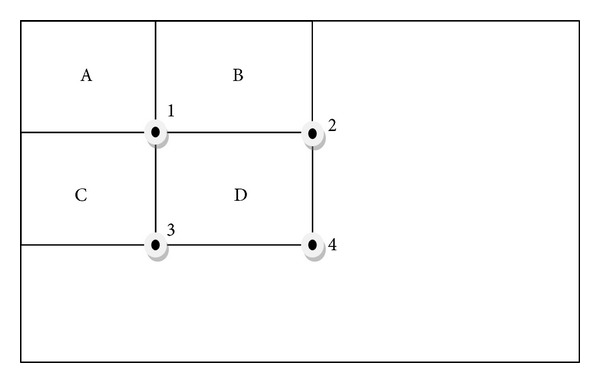
\includegraphics[scale=1.0]{imgs/sumPixels.png}
	\caption{Obliczanie sumy wartości pikseli Źródło: \cite{sumPixelsDoc}}
	\label{fig:obrazScalkowany}
\end{figure}

Rysunek \ref{fig:obrazScalkowany} przedstawia schemat obrazu, po transformacji do obrazu scałkowanego dla którego próbujemy wyznaczyć sumę pikseli w wewnętrznym prostokącie. W celu obliczenia sumy pikseli dla zaznaczonego prostokąta D musimy uwzględnić wartości sum 4 prostokątów. Suma pikseli dla prostokąta A jest równa wartości zdjęcia scałkowanego w punkcie 1,
Analogicznie w punkcie 2 opisuje wartość sumy dla prostokąta A + B, w punkcie 3 dla prostokąta A + C, natomiast w punkcie 4 dla prostokąta A + B + C + D. Do wyznaczenia sumy pikseli w prostokącie D potrzebujemy zatem wartości zdjęcia scałkowanego w punktach opisującym ten prostokąt. I tak dla przedstawionego schematu suma pikseli w prostokącie D jest równa 4 - 2 -3 + 1.
Wyznaczenie tej wartości dla każdego prostokąta zatem zawsze jest wykonane w stałym czasie, są to zawsze te same operacje dodawania i odejmowania.

\subsection{Proces uczenia mocnych klasyfikatorów}\label{uczenieMocnych}

Każdy klasyfikator włączony do kaskady jest złożony z wielu tzw. Słabych klasyfikatorów. Każdy z nich jest pojedynczą cechą Haar’a która została włączona do klasyfikatora w procesie uczenia. Pojedynczy klasyfikator zwykle nie jest w stanie jednoznacznie sklasyfikować obiektu. W celu usprawnienia skuteczności detekcji za pomocą cech stosuje się tak zwany Boosting. Celem tego zabiegu jest stworzenie klasyfikatora, którego ocena będzie składała się z ocen wielu klasyfikatorów odpowiednio przeskalowane w stosunku do ich skuteczności określonym w etapie uczenia. 

\begin{figure}[H]
	\centering
	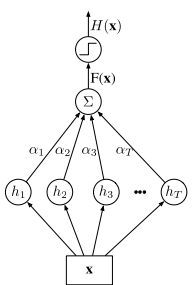
\includegraphics[scale=0.6]{imgs/mocny.png}
	\caption{Działanie mocnego klasyfikatora Źródło: \cite{AdaBoostClasifire}}
	\label{fig:klasyfikatorMocny}
\end{figure}

Rysunek \ref{fig:klasyfikatorMocny} przedstawia działanie mocnego klasyfikatora. Na wejściu podane jest zdjęcie X które jest analizowane przez każdą cechę $h$. Następnie wynik każdej cechy (możliwe \{1, -1\}) jest mnożony przez jej współczynnik, na koniec wyniki są sumowane. Obliczona suma większa od zera oznacza, że klasyfikator odnalazł obiekt, w przeciwnym razie analizowany fragment nie został sklasyfikowany jako szukany element.

Mocne Klasyfikatory otrzymywane są w procesie uczenia maszynowego. Trening klasyfikatorów odbywa się w oparciu o zbiór danych uczących. W skład takiej bazy będą wchodziły zdjęcia, na których znajduje się szukany obiekt, tak zwane zdjęcia pozytywne, oraz zdjęcia na których nie ma obiektu, tak zwane zdjęcia negatywne. Dodatkowo dane muszą posiadać etykiety które informują czy na zdjęciu znajduje się obiekt czy też nie. W tym przypadku kaskady Haar’a są otrzymywane poprzez implementacje algorytmu AdaBoost jest to jeden ze sposobów uczenia z nadzorem. To iteracyjny algorytm, w każdej iteracji wybierany  jest jeden słaby klasyfikator w tym przypadku cecha Haar’a, która najskuteczniej klasyfikuje obiekt. Dene, które zostały źle sklasyfikowany przez wybraną cechę zostają obciążone większymi wagami, by w następnych iteracjach kolejne klasyfikatory musiały radzić sobie szczególnie dobrze ze zdjęciami błędnie oznaczonymi przez poprzednio wybrane cechy. Tak dobrane słabe klasyfikatory łącznie tworzą silny klasyfikator, który jest włączany do kaskady. Na wejście algorytmu podany jest zestaw danych uczących wraz z etykietami \{$x_{i}$, $y_{i}$\} $x_{i}$ jest kolejnym zdjęciem a $y_{i}$ jest etykietą \{1, -1\}. Zbiór danych liczy n elementów.

\begin{algorithm}[H]
	\caption{AdaBoost}\label{adaBoost}
	\begin{algorithmic} 
		\DontPrintSemicolon
		\STATE $D_k(i)$: \tcp*{przykładowa waga elementu $i$ klasyfikatora $k$}
		\STATE $\alpha_k$:\tcp*{ waga klasyfikatora $k$}
		\STATE $\forall_i$: $D_1(i) \gets$ ${1} \over {n}$ \tcp*{początkowe wagi danych}
		\FOR{$k = 1$ \TO $K$ } 
		\STATE $\forall h$ $\epsilon_k \gets$ $\sum_{i:y\neq h(x_i)}^{} $ $D_k(i)$ \tcp* {obliczanie błędu dla każdego klasyfikatora}
		\STATE $h_k \gets argmin(\epsilon_k(h))$ \tcp* {wybór klasyfikatora z najmniejszym błędem}
		\IF{$\epsilon_k \geq$ $1 \over 2$} 
		\STATE stop \tcp*{jeśli klasyfikator ma 50\% błędu to stop}
		\ELSE
		\STATE $\alpha_k \gets $ $1 \over 2$ $1- \epsilon_k \over \epsilon_k$
		\STATE $D_{k+1}(i) \gets$ $D_k(i)e^{-y_i\alpha_k h_k(x_i)} \over Z_k$
		\ENDIF
		\ENDFOR
		\STATE $H_{final}(x) = sgn(\sum_{k=1}^{K} \alpha_k h_k(x))$
	\end{algorithmic}
\end{algorithm}

Ocena skuteczności klasyfikatora opiera się na tak zwanej macierzy pomyłek (z ang. Confusion Matrix), która definiuje współczynniki określające:
\begin{itemize}
	\item Liczba dobrych klasyfikacji jako obiekt
	\item Liczba złych klasyfikacji jako obiekt
	\item Liczba dobrych klasyfikacji jako nie obiekt
	\item Liczba złych klasyfikacji jako nie obiekt
\end{itemize}

Na podstawie tych danych obliczany jest współczynnik dobrze sklasyfikowanych obiektów w stosunku do liczby zdjęć pozytywnych, dalej określany jako TPR ( z ang. true positive rate). Obliczany jest także współczynnik błędnych decyzji jako stosunek liczby błędnie sklasyfikowanych jako obiekt do liczby zdjęć negatywnych, dalej określany jako FPR (z ang. false positive rate)

\subsection{Kaskada klasyfikatorów mocnych}
W celu dodatkowego poprawienia skuteczności zaproponowano zastosowanie kaskady klasyfikatorów, która jest czymś na wzór drzewa decyzyjnego. Każdy z mocnych klasyfikatorów otrzymanych na podstawie działania algorytmy AdaBoost jest jednym z elementów kaskady. Aktualnie poszukiwany obszar jest sprawdzany przez kolejne klasyfikatory. Na wejście kaskady podawany jest analizowany obszar. Pierwszy klasyfikator analizuje fragment wszystkimi cechami które wchodzą w jego skład. Jeśli klasyfikator stwierdzi że we wskazanym obszarze znajduje się obiekt fragment zostaje poddany analizie przez następny klasyfikator w kaskadzie. Jeśli fragment zostanie niesklasyfikowany przez któryś element kaskady zostaje podjęta jednoznaczna decyzja dla całej kaskady o braku obiektu. O obecności szukanego wzorca w kaskadzie, muszą wskazać wszystkie elementy kaskady. Podczas uczenia kolejne etapy wybierają do klasyfikatora mocnego cechy z coraz mniejszej puli jest ich zatem coraz więcej w kolejnych elementach kaskady. 

Sama detekcja jest oparta na sprawdzaniu kolejnych fragmentów zdjęcia przesuwając miejsce badanego fragmentu po całym obrazie. Analiza fragmentów, które są tłem obiektu trwa stosunkowo krótko ponieważ o braku obiektu powinny stwierdzić pierwsze elementy kaskady, które składają się z mniejszej ilości cech niż końcowe etapy. Analiza przy użyciu końcowych etapów kaskady jest wykorzystana prawie tylko w przypadku badania fragmentu na którym znajduje się obiekt.
Kosztowna analiza za pomocą wszystkich cech wchodzących w skład kaskady zazwyczaj jest wykonywana tylko dla mniejszej części zdjęcia, co sprawia, że algorytm jest szybki.
 \newpage
\section{Wykorzystanie biblioteki OpenCV (Maciej Plewka)}\label{sec:opencv}
Biblioteka OpenCV to otwarte oprogramowanie, które jest wykorzystywane do przetwarzania zdjęć. Jest to narzędzie wspierane przez Windows, GNU/Linux, macOS oraz Android. W naszej pracy biblioteka została wykorzystana na systemie Ubuntu jednej z wielu dystrybucji systemu Linux w celu wytrenowania własnej kaskady oraz testowania a także na platformie Android by wykorzystać wytrenowane modele zaraz po wykonaniu zdjęcia aparatem. Źródła biblioteki są publicznie dostępne w zdalnym repozytorium \cite{OpenCVSource}. Narzędzia OpenCV umożliwiają wykorzystanie standardu OpenCL który pozwala na równoległe obliczenia z użyciem procesorów centralnych oraz graficznych.


\subsection{OpenCV w procesie trenowania kaskad}

OpenCV oprócz zestawu funkcji operacji na obrazach dostarcza także aplikację pozwalającą na wytrenowanie własnej kaskady cech Haar’a jest to opencv\_traincascade oraz kilka aplikacji które wspierają ten proces to takie aplikacje jak opencv\_createsamples który pozwala stworzyć zbiór uczący na podstawie pojedynczego pozytywnego zdjęcia, opencv\_visualisation umożliwia wizualizację cech włączonych do kaskady w odniesieniu do podanego zdjęcia ze wzorem obiektu którego detekcji uczymy.

\subsubsection{Generowanie zbioru zdjęć pozytywnych}\label{sec:generowanieZdjec}
Przed rozpoczęciem trenowania naszej kaskady klasyfikatorów potrzebne są zdjęcia na których umieszczony jest  obiekt który ma być rozpoznawany oraz kolekcje zdjęć na których nie ma naszego wzorca. By kaskada została skutecznie wytrenowana potrzebne jest jak najwięcej zdjęć. Do wytrenowania kaskady, która rozpoznaje twarze, dołączonej wraz z biblioteką OpenCV wykorzystano 3000 zdjęć pozytywnych oraz 1500 zdjęć negatywnych. Jasnym problemem staje się wykonanie takiej liczby zdjęć na których znajduje się wybrany obiekt a następnie oznaczyć dokładnie jego położenie. Do stworzenia zbioru zdjęć pozytywnych wykorzystano aplikacje opencv\_createsaples. Program ten pozwala na wygenerowania zbioru zdjęć pozytywnych na podstawie jednego zdjęcia na którym tylko i wyłącznie znajduje się przedmiot który potem będzie szukany. Zdjęcie to zostaje umieszczone na każdym zdjęciu w losowych miejscach o losowym rozmiarze i o losowym przesunięciu w każdej z trzech płaszczyzn. Dobór zdjęć nie jest dowolny, ważne aby na zdjęciach na które zostanie nałożony nasz obiekt . Ostatnim elementem potrzebnym do skorzystania z aplikacji opencv\_createsamples jest przygotowanie pliku tekstowego w którym wylistowane będą ścieżki do plików na które mają zostać naniesione wzory naszego obiektu. Dla tak przygotowanych danych możemy uruchomić aplikacje opencv\_createsamples wraz ze wskazanymi parametrami:
\begin{itemize}
    \item -img \textless ścieżka do wzorcowego zdjęcia \textgreater
    \item -bt \textless ścieżka do pliku z opisem zdjęć tła\textgreater
    \item -info \textless ścieżka do pliku w którym mają być zapisane informacje o utworzonych zdjęciach\textgreater
    \item -pngout \textless ścieżka do katalogu w jakim mają być zapisywane pozytywne zdjęcia\textgreater
    \item -bgcolor \textless ośmiobitowa wartośćkoloru tła\textgreater
    \item -bgtrash \textless zakres wartości koloru\textgreater
    \item -maxxangle \textless maksymalny kąt w płaszczyźnie x wyrażony w radianach\textgreater
    \item -maxyangle \textless maksymalny kąt w płaszczyźnie y wyrażony w radianach\textgreater
    \item -maxzangle \textless maksymalny kąt w płaszczyźnie z wyrażony w radianach\textgreater
    \item -num \textless liczba zdjęć która ma zostać wygenerowana>

\end{itemize}

Po uruchomieniu aplikacji we wskazanym folderze zostaną wygenerowane pozytywne zdjęcia 

\begin{figure}[H]
\centering
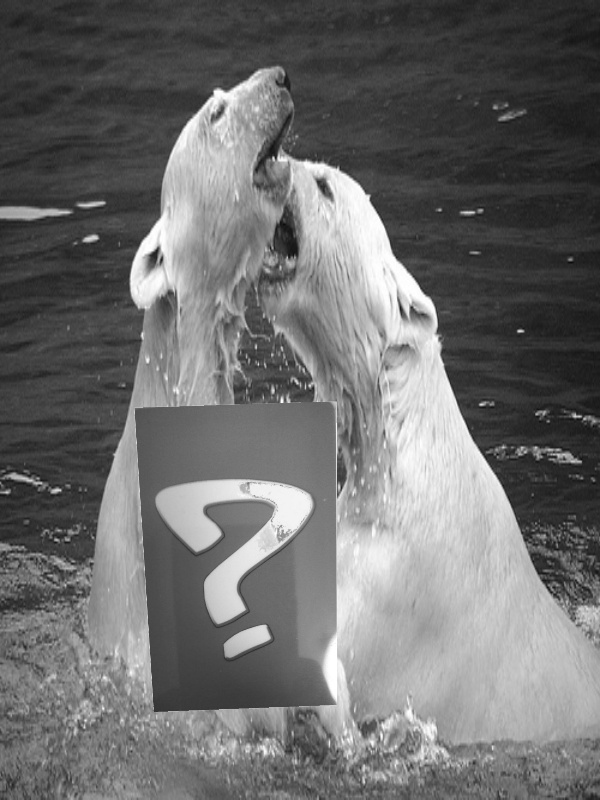
\includegraphics[scale=0.2]{imgs/0448_0134_0398_0203_0316.png}
\caption{Wygenerowane pozytywne zdjęcie}\label{misie}
\end{figure}

Rysunek \ref{misie} przedstawia przykładowo wygenerowane pozytywne zdjęcie. Informacje na temat zdjęcia zapisane we wskazanym pliku info dla tego zdjęcia wygląda następująco
0185\_0196\_0219\_0293\_0454.jpg 1 196 219 293 454
Elementy kolejno oznaczają:

\begin{itemize}
    \item Nazwa pliku
    \item Liczba obiektów na zdjęciu
    \item Współrzędna x lewego górnego rogu obiektu na zdjęciu
    \item Współrzędna y lewego górnego rogu obiektu na zdjęciu
    \item Szerokość obiektu
    \item Wysokość obiektu

\end{itemize}

Posiadając plik info z informacjami na temat położenia zdjęć możemy uzyskać plik z rozszerzeniem vec, który następnie będzie używany przez aplikacje trenującą kaskadę. Posłuży nam do tego także aplikacja opencv\_createsamples. Tym razem należy wskazać następujące parametry:

\begin{itemize}
    \item -info \textless sciezka do pliku info w którym znajdują się informacje o obiektach \textgreater
    \item -vec \textless ściezka do pliku w jakim ma być zapisany plik vec\textgreater
    \item -num \textless ilość zdjęć jaka ma być zapisana w pliku vec\textgreater
    \item -w \textless zerokość obiektu\textgreater
    \item -h \textless wysokość obiektu\textgreater

\end{itemize}

\subsubsection{Trening kaskady}

Do treningu kaskady wykorzystujemy aplikacje opencv\_traincasscade, która implementuje algorytm opisany w punkcie 3.3 . Aplikacja zostanie uruchomiona z następującymi parametrami:

\begin{itemize}
    \item -vec \textless ścieżka do pliku z wektorem opisującym pozytywne zdjęcia \textgreater
    \item -bg \textless sciezka do pliku z zapisanymi ścieżkami plików tworzących zbiór zdjęć negatywnych \textgreater
    \item -numPos \textless liczba pozytywnych zdjęć użyta do treningu \textgreater
    \item -numNeg \textless liczba zdjęć negatywnych użytych do treningu \textgreater
    \item -w \textless szerokość obiektu, taka sama jak w podanym pliku vec \textgreater
    \item -h \textless wysokość obiektu, taka sama jak w podanym pliku vec \textgreater
    \item -numStages \textless liczba elementów z których ma się składać kaskada \textgreater
    \item -maxyangle \textless maksymalny kąt w płaszczyźnie y wyrażony w radianach\textgreater
    \item -maxzangle \textless maksymalny kąt w płaszczyźnie z wyrażony w radianach\textgreater
    \item -num \textless liczba zdjęć która ma zostać wygenerowana>

\end{itemize}

Te parametry są niezbędne do uruchomienia treningu za pomocą tej aplikacji. Możliwe do podania są także inne parametry, które deklarują inną dokładność słabych i silnych klasyfikatorów niż zdefiniowanych domyślnie przez aplikacje. W przypadku podania parametrów które stwierdzają większość dokładność algorytm prawdopodobnie będzie bardziej skuteczny lecz trening będzie trwał dłużej. Natomiast przy zmniejszeniu czas treningu ulegnie skróceniu. Te parametry to:
 
\begin{itemize}
    \item -minHitRate \textless minimalna wartość współczynnika oznaczającego pozytywne klasyfikacje \textgreater
    \item -maxfalsealarm \textless maksymalna dopuszczalna wartość błędnych decyzji \textgreater

\end{itemize}

Podczas trenowania kaskady przydatna jest także aplikacja opencv\_visualisation, która da dotychczasowych etapów generuje podgląd dobranych cech na tle obiektu. Program ten przyjmuje następujące parametry:

\begin{itemize}
    \item -data \textless ścieżka do wygenerowanych obrazów z naniesionymi cechami \textgreater
    \item -image \textless zdjęcie obiektu o rozmiarze takim jaki podany do uczenia kaskady \textgreater
    \item -model  \textless ścieżka do pliku xml z wytrenowanym dotychczas modelem kaskady \textgreater

\end{itemize}

Po uruchomieniu aplikacji zostaną wygenerowane pliki zdjęciowe, osobno dla każdego etapu kaskady. Na każdym z utworzonych obrazów znajduje wizualizacja osobno wszystkich cech wchodzących w skład danego etapu. Obok zdjęć generowany jest także plik wideo w formacie avi na którym przedstawione są po kolei wszystkie cechy wchodzące w skład kaskady na tle obiektu

\begin{figure}[H]
\centering
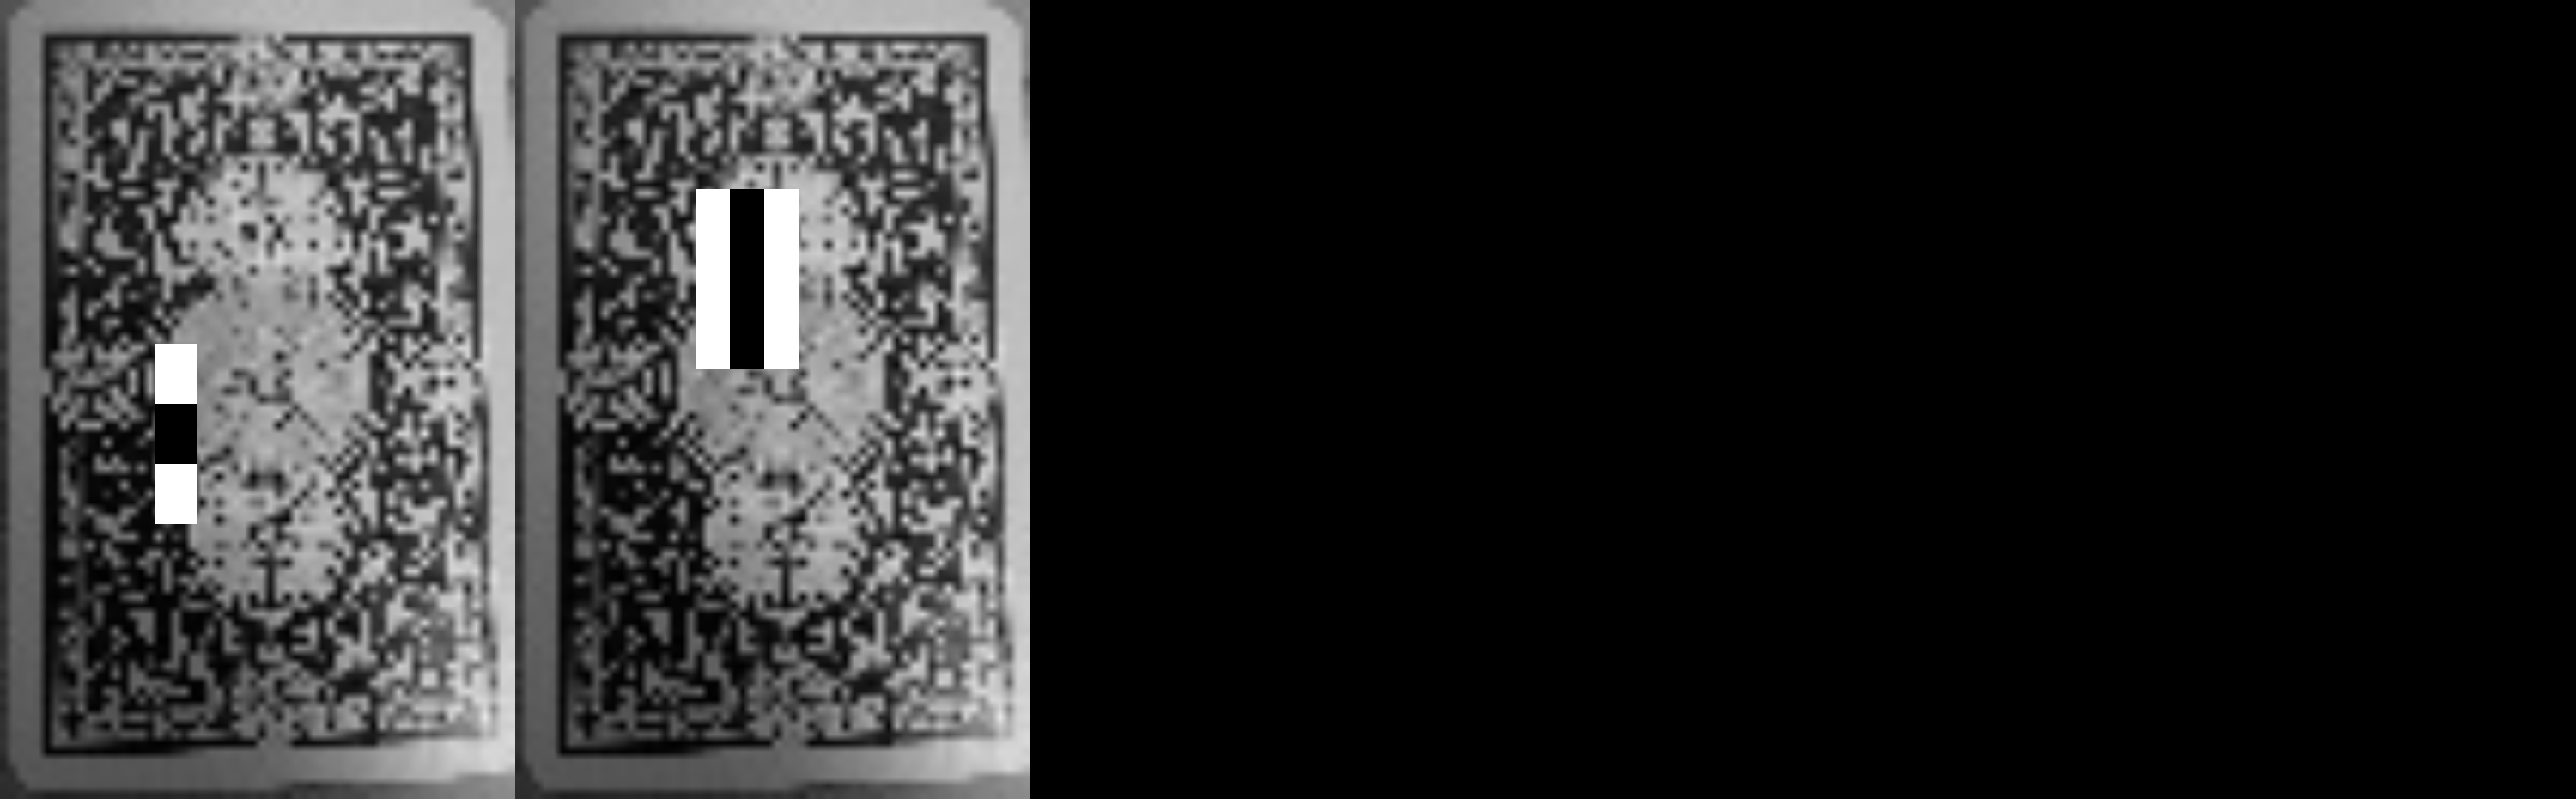
\includegraphics[scale=0.1]{imgs/data3stage_1.png}
\caption{Cechy mocnego asyfikatora}
\end{figure}

\subsection{OpenCV na platformie Android}

Biblioteka OpenCV dla Androida dostarczona jest w zestawie narzędzi deweloperskich OpenCV. Daje ona api Javy. Posiada on prawie wszystkie funkcjonalności Javy. Wszystkie operacje wykonywane są przy użyciu natywnych metod zaimplementowanych w języku C++. Istnieją dwa podejścia w wykorzystaniu tej biblioteki pierwsze zakłada wołanie funkcji poprzez dostarczone api Javy pozwalające bezpośrednio i w łatwy sposób wykorzystanie funkcji w celu przetwarzania obrazu. Wadą takiego podejścia jest wykorzystanie metod JNI, które trwają stosunkowo długo, do tego dochodzi kwestia kopiowania i mapowania obiektów co także mocno wykorzystuje zasoby. Drugie podejście zakłada użycie metod biblioteki z poziomu funkcji natywnych. Zastosowanie takiego rozwiązania jest korzystne jeśli w konkretnym bloku wykonujemy szereg funkcji które z poziomu kodu java wołały by także metody jni. W tym wypadku tak wołana metoda byłaby tylko raz a reszta funkcji wołana by była juz z niskiego poziomu. Takie rozwiązanie jest szybsze oraz wykorzystuje mniej zasobów. Dodatkowo w przypadku wywoływania metod z niskiego poziomu mamy dostęp do 100\% funkcji dostarczanych przez bibliotekę. Jest to rozwiązanie bardziej skomplikowane, trzeba także pamiętać o odpowiednim zarządzaniu pamięcią, gdyż garbage collector działa tylko w ramach maszyny wirtualnej java.

\subsubsection{Detekcja obiektów}

Cały proces detekcji odbywa się przy użyciu kilku funkcji z biblioteki openCV. Na początku należy wczytać zdjęcie. W zależności od źródła zdjęcia może być ono odczytane np jako pojedyncza klatka z kamery lub tak jak w naszym przypadku weźmiemy pojedyncze zdjęcie z pamięci urządzenia. Służy do tego metoda imread wywoływana na obiekcie Imgcodecs. Parametrami tej funkcji są ścieżka do pliku zdjęciowego oraz parametr oznaczający format w jakim ma byc odczytane zdjęcie takimi formatami są:
\begin{itemize}
    \item CV\_LOAD\_IMAGE\_UNCHANGED (\textless0) ładuje zdjęcie w takim formacie w jakim oryginalnie jest zapisane.
    \item CV\_LOAD\_IMAGE\_GRAYSCALE ( 0) ładuję zdjęcie w skali szarości
    \item CV\_LOAD\_IMAGE\_COLOR (\textgreater0) ładuję zdjęcie w formacie BGR
\end{itemize}
Do późniejszej detekcji potrzebujemy zdjęcie wczytane w skali szarości dlatego wczytujemy z parametrem cv2.IMREAD\_GRAYSCALE.
Załadowane zdjęcie znajduje się w obiekcie klasy Mat. Jest to klasa przechowująca macierze oraz obrazy. Posiada wiele właściwości opisujące zdjęcie takie jak np rozmiar.
Do detekcji potrzebujemy załadować także nasz plik z kaskadą w formacie xml. Tworzymy obiekt klasy CascadeClassifier, w konstruktorze obiektu podajemy ścieżkę do naszego wytrenowanego modelu. Kiedy mamy przygotowany obraz oraz kaskadę możemy na kaskadzie zawołać metodę detectMultiScale która w parametrach przyjmuje obiekt Mat w którym znajduje się załadowane zdjęcie na którym szukamy obiektu, referencja do kolekcji MatOfRect do którego zostaną zapisane fragmenty zdjęcia z szukanym obiektem, scaleFactor to następny parametr, który określa zmianę wielkość przeszukiwanego fragmentu w kolejnych iteracjach algorytmu. Wysoka wartość tego parametru sprawia, że różnica między klasyfikatorami w kolejnych iteracjach jest większa. Mała wartość parametru sprawia, że większa ilość fragmentów zostanie przeszukana co sprawia, że detekcja trwa długo. Wysoka wartość przyspiesza znacząco czas działania algorytmu lecz istnieje możliwość pominięcia przeoczenia szukanego elementu. Kolejny parametr to minNeighbors który określa minimalną ilość sąsiednich fragmentów uznanych jako wykryty obiekt, żeby uznać go za pozytywny. Kolejne parametry to obiekty typu size określające minimalną wielkość i maksymalną wielkość szukanego obiektu. Jeśli różnica tych wielkości jest duża czas algorytmy się wydłuży gdyż więcej różnych wielkości będzie musiało zostać sprawdzonych. 
Po wykonaniu metody detectMultiScale kolekcji MatOfRect zapisane są informacje o współrzędnych odnalezionych obiektów,w tych miejscach możemy wkleić prostokąt lub w jakiś inny sposób modyfikować.
 \newpage
\section{Trening własnej kaskady}

W celu zrealizowania detekcji naszej własnej karty, potrzebne było wytrenowanie własnej kaskady klasyfikatorów Haar'a. W tym celu skorzystano z aplikacji dostarczonych przez openCV szerzej opisanych w rozdziale \ref{sec:opencv}. Cały proces uczenia został wykonany na komputerze osobistym z procesorem Intel Core i3 4000M o częstotliwości taktowania zegara 2,4 GHz i 8GB pamięci operacyjnej. Biblioteka OpenCV wraz z aplikacjami zostały skompilowane ze źródeł znajdującym się w publicznym repozytorium \cite{OpenCVSource}. Dodatkowo podczas budowania biblioteki zaznaczono flagę by zostało włączone wspieranie standardu OpenCL, który umożliwia zrównoleglenie obliczeń co znacząco przyspiesza czas działania zbudowanych aplikacji.

\subsection{Zbiór danych uczących}

Zdobycie przynajmniej 2000 zdjęć wykorzystanych do uczenia jest dużym problemem. Dlatego dane uczące zostały wygenerowane przy użyciu aplikacji opencv\_createsamples, opisanej w rozdziale \ref{sec:generowanieZdjec}. Do wygenerowania zdjęć pozytywnych wykorzystano 5 zdjęć na których znajduje się tylko i wyłącznie nasz wzór. W pierwotnych założeniach rozpoznawany miał być rewers wybranej karty. Z powodu skomplikowanego wzoru rewersu karty, gdzie kolor biały i czarny gęsto się przeplata, postanowiono proces treningu przeprowadzić także na własnej, przygotowanej karcie, której wzór jest stosunkowo prosty. Potrzebny był także zbiór zdjęć na którym nie znajduje się nasza karta. Wykorzystano do tego serwis internetowy \cite{imageNetOrg}, który posiada bogaty zbiór sklasyfikowanych zdjęć, udostępniony z intencją wykorzystania do uczenia maszynowego. Z tej bazy zdjęć pobrano niecałe 3000 zdjęć sklasyfikowanych jako niedźwiedzie, robaki, gitary, pociągi i książki. Zbiór tych zdjęć pogrupowano na 5 podgrup po 500 zdjęć. W celu skrócenia czasu treningu zdjęcia te zostały zmniejszone za pomocą funkcji resize biblioteki openCv, która wykorzystuje interpolacje. Jest to proces który dzięki któremu wyznaczamy wartość nowego piksela na podstawie innych sąsiadującym z nim pikseli. Zdjęcia tła zostały zmniejszone do rozdzielczości 120x186 pikseli. Jest to wymiar którego stosunek wysokości i wysokości jest taki sam jak wielkości karty. Obrazy wzorów kart zostały również pomniejszone, jednak te do rozdzielczości 40x62. Z początku rozważano użycie mniejszej wielkości zdjęć co spowodowałoby zmniejszenie liczby możliwych cech Haar'a dla obiektu jednak dość skomplikowany wzór awersu karty powodował nieczytelność zdjęcia a co za tym idzie cechy słabo generalizowały by odpowiednie fragmenty prawdziwego obiektu. Wszystkie wykonane operacje dla obu wzorów dalej będą wykonywane analogiczne, z tymi samymi parametrami.

\begin{figure}[H]
\centering
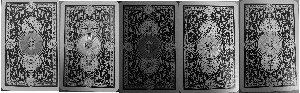
\includegraphics[scale=1.0]{imgs/RewersyKarty.jpg}
\caption{Rewersy kart użyte do treningu}
\label{fig:KartaRewers}
\end{figure}
.

\begin{figure}[H]
\centering

\includegraphics[scale=1.2]{imgs/Karta?.jpg}
\caption{Wzory własnej karty użyte do treningu}
\label{fig:KartaTajemnicza}
\end{figure}

Zdjęcia zostały podzielone na 5 katalogów, by każdy z nich odpowiadał jednemu obrazowi wzoru. By utworzyć zbiór zdjęć pozytywnych potrzebujemy jeszcze pliku tekstowego w którym wylistowane będą ścieżki do zdjęć będących tłem wybranego wzoru. Posiadając wszystkie wymagane pliki tj. Zdjęcie z pozytywnym wzorem, plik tekstowy ze ścieżkami do obrazów tła. Możemy uruchomić aplikacje opencv\_createsamples. Dodatkowo ustawiono losowy kąty nachylenia na do 0,2 rad w płaszczyźnie x oraz y natomiast w płaszczyźnie z do 0,1 rad. Dodatkowo koniecznym było ustawienie odpowiedniego koloru tła naszego pozytywnego zdjęcia. Nasze pozytywne wzory nie zawierają tła dlatego, jednak domyślnie za kolor tła jest brana wartość 0 tj. kolor czarny co w przypadku obu kart powoduje ignorowanie niektórych fragmentów powodując że są ona jakby przezroczyste. Kolor tła w tej aplikacji określany jest jako zakres obliczany z wartości parametrów bgcolor oraz bgthresh. Jako tło brany jest każdy kolor z przedziału od bgcolor-bgthresh do bgcolor+bgthresh. W naszych wzorach tło nie występowało więc jako parametr -bgcolor podano 200 tj kolor nie znajdujący się na naszym wzorze a -bgtresh przyjęto wartość 1. Po uruchomieniu aplikacji posiadamy 2500 sklasyfikowanych zdjęć pozytywnych na których znajdują się wzory których detekcje chcemy osiągnąć. Teraz dla każdego pliku info z informacjami na temat wygenerowanych obrazów możemy wygenerować plik z rozszerzeniem vec, który jest potrzebny do poprawnego uruchomienia aplikacji trenującej kaskadę klasyfikatorów.
Polecenie które uruchomiło wygenerowanie obrazów dla jednego pozytywnego zdjęcia i 500 zdjęć będących tłem wygląda następująco:
\begin{lstlisting}
opencv\_createsamples -img pos?/pos5.jpg -bg bg5.txt -info info/info5.list -pngoutput info/ -bgcolor 200 -bgthresh 1 -maxxangle 0.2 -maxyangle 0.2 -maxzangle 0.1 -num 500 -w 40 -h 62
\end{lstlisting}


Aplikacja została uruchomiona dla pięciu różnych zdjęć karty. Kolejne polecenia uruchamiające różniły się wskazaniem na inne zdjęcie wzorca, inny plik ze ścieżkami zdjęć będących tłem oraz innym plikime info do którego zapisywane są informacje o wygenerowanych zdjęciach.
Ostatnim krokiem kończącym proces przygotowania danych jest połączenie pięciu plików vec w jeden, który będzie jednym z argumentów wejścia programu opencv\_traincasscade. Wykożystujemy do tego skrypt mergevec.py \cite{mergeVec}. Narzędzie to przyjmuje dwa argumenty:
\begin{itemize}
    \item -v \textless Sciezka do katalogu z plikami vec które należy scalić \textgreater
    \item -o \textless nazwa scalonego wynikowego pliku \textgreater
\end{itemize}
Pliki vec skopiowano do katalogu vec, skrypt mergevec.py znajduje się w katalogu mergevec. Polecenie które wygenerowało scalony plik vec wygląda następująco: 
\begin{lstlisting}
    python mergevec/mergevec.py -v vec/ -o posss.vec
\end{lstlisting}
\subsection{Proces treningu}

Proces treningu kaskady przeprowadzono dla dwóch wzorów. Jednym znich jest rewers karty, z talii kart do gier karcianych, drugi to przygotowany przez nas wzór przedstawiający znak zapytania na czerwonym tle. Dla każdego wzorca proces uczenia odbywał się na podstawie zdjęć wygenerowanych i przeskalowanych to tej samej wielkości. Początkowo zakładano by rozmiar wzorców wynosił 20x31 pikseli, by obniżyć do minimum liczbę możliwych cech Haar'a.
Po przeskalowaniu zdjęć do określonej wielkości okazało się, że rewers kart jest bardzo niewyraźny co ogranicza zdolność cech do generalizowania. Dlatego rozmiar wzorców ustalono na 40x62 pikseli. Wymiar ten zachowuje proporcje naszych kart. Liczba unikalnych cech Haar'a dla takiego rozmiaru wynosi 2978000. Rysunki \ref{fig:KartaTajemnicza} i \ref{fig:KartaRewers} przedstawiają wzory użyte do treningu kaskad po przeskalowaniu. Przeprowadzony trening odbywał się na zbiorze 1800 zdjęć pozytywnych oraz 900 zdjęciach negatywnych. Obrazy te posiadały jednakowy rozmiar 120x186. Zastosowano taki rozmiar by skrócić czas treningu, ponieważ dla większego zdjęcia podczas treningu trzeba przeanalizować większą ilość fragmentów. By zapobiec przeuczeniu tj. sytuacji w której kaskada będzie wytrenowana tylko i wyłącznie do rozpoznawania zdjęć treningowych, postanowiono ograniczyć się do wygenerowania 12 etapów kaskady. Do uruchomienia aplikacji potrzebne są juz wygenerowany plik vec. Współczynniki pozytywnych decyzji i negatywnych zostały zastosowane takie jak domyślne wartości aplikacji TPR = 0.995 a FPR = 0.5. Komenda uruchamiająca trening dla obu wzorów wygląda następująco:

opencv\_traincascade -data data -vec posss.vec -bg bgall.txt -numPos 1800 -numNeg 900 -numStages 11 -w 40 -h 62

\subsubsection{Trening detercji rewersu karty}

Ze względu na pierwotne założenia pierwszym wzorem na którym był przeprowadzony proces detekcji był rewers karty. Proces uczenia trwał 38 godzin wytrenowana kaskada składa się z 12 etapów i posiada 98 klasyfikatorów słabych opisujących wzór karty.

\begin{figure}[H]
\centering
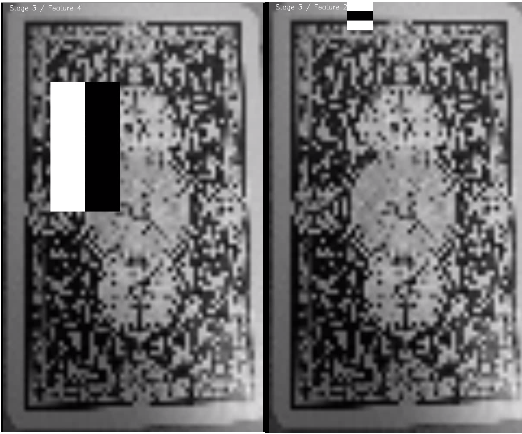
\includegraphics[scale=0.2]{imgs/cechyRewers.png}
\caption{Cechy opisujące rewers karty}
\label{fig:cechyRewers}
\end{figure}

Rysunek \ref{fig:cechyRewers} przedstawia przykładowe cechy włączone do kaskady celnie opisujące wzór. Wytrenowana kaskada słabo radzi sobie z jednoznaczną detekcją obiektów. Na 10 zdjęć na których znajduje się tylko i wyłącznie karta na różnych tłach tylko na dwóch z nich celnie odnaleziono obiekt. Dodatkowo w obrębie karty odnalazł także kilka obiektów, więc na żadnym ze zdjęć nie był w stanie jednoznacznie wskazać obiektu. Powodem takiego wyniku jest najprawdopodobniej skomplikowany wzór, który gęsto przeplata biały i czarny kolor. Spowodowało to, że cechy pasują do różnych miejsc w obrębie karty, przez co nie jest w stanie jednoznacznie odnaleźć obiektu. Kolejnym elementem wpływającym niekorzystnie na detekcję jest pomniejszony obraz wzoru. Spowodowało to, że cechy odzwierciedlają wyraźnie zniekształconą wersję obiektu.

\subsubsection{Trening detekcji karty ze znakiem zapytania}

Z powodu słabej skuteczności kaskady przeznaczonej do detekcji rewersu karty postanowiono użyć innego wzoru. Słaba skuteczność spowodowana była najprawdopodobniej skomplikowanym wzorem. Trening kaskady został uruchomiony z takimi samymi parametrami jak w przypadku rewersu karty. Cały proces uczenia zajął 11 godzin. Kaskada składa sie z 11 etapów, ponieważ po 11 etapie, ponieważ współczynnik FPR osiągnął już zadowalający poziom. Kaskada składa się z 54 cech Haar'a.

\begin{figure}[H]
\centering

\includegraphics[scale=0.2]{imgs/cechy?.png}
\caption{Cechy opisujące naszą kartę}
\label{fig:cechy?}
\end{figure}

Rysunek \ref{fig:cechy?} przedstawia przykładowe cechy celnie opisujące naszą kartę. Na 10 zdjęć zawierających tylko i wyłącznie szukany obiekt na wszystkich obiekt został poprawnie sklasyfikowany, przy czym na trzech z nich zostały także wskazane elementy kompletnie nie związane z szukanym wzorem. Otrzymano zatem 7 jednoznacznych decyzji o odnalezieniu obiektu, można powiedzieć, że osiągnięto sukces.
 \newpage
\section{Użycie Kaskad w celu realizacji Tricku (Maciej Plewka)}

W tym rozdziale opisany zostanie sposób użycia kaskady do zrealizowania dwóch wariantów sztuczki. Pierwszy to ten w którym wklejana jest karta w miejsce odnalezienia czoła, w drugim przypadku zamieszczamy ją w miejsce wyznaczonego obiektu. Opisany także będą sposoby dzięki którym osiągnięto optymalną skuteczność.

\subsection{Detekcja Czoła}

W celu detekcji czoła wykorzystano kaskady zapisane w plikach w plikach z rozszerzeniem xml, które są dołączone razem z biblioteką openCV. Wykorzystano plik kaskadowy pliki lbpcascade\_frontalface.xml oraz haarcascade\_lefteye\_2splits.xml.
Pierwszy z nich opisuje klasyfikatory służąca do rozpoznawania przodu twarzy, drugi 
Teoretycznie służy do detekcji lewego oka które jest otwarte. Kaskada służąca do rozpoznawania lewego oka w praktyce jest wstanie skutecznie rozpoznać także prawe oko a także jeśli chcemy wykorzystać ją do detekcji obu oczu radzi sobie lepiej niż kaskada odpowiedzialna za prawe oko. W naszej aplikacji miejsce czoła zostaje wyznaczone na podstawie informacji na temat położenia twarzy oraz oczu. Wykrywanie oczu zostaje uruchomione w momencie rozpoznania twarzy, gdyż wiadomym jest, że do poprawnego wykrycia oczu muszą się one znajdować w twarzy. 
Następnie, jeśli udało się nam odnaleźć w zdjęciu twarz a w niej parę oczu uznajemy że detekcja przebiegła poprawnie. Zwrócone obiekty są typu Rect jest to typ z biblioteki openCV. W tym momencie wyznaczamy matematycznie domniemane miejsce czoła na podstawie położenia na zdjęciu twarzy oraz oczu. Lecz zanim określimy dokładne miejsce czoła należy określić które oko znajduje się po lewej.
Za lewy dolny punkt czoła przyjmiemy lewy górny punkt oka znajdującego się po lewej stronie, natomiast prawy dolny punkt jest równy co do wartości prawemu górnemu rogowi oka prawego. Różnica tych wartości jest zatem szerokością czoła. Wysokość czoła jest to szerokość czoła podzielona przez 2 albo jeśli wyznaczona w ten sposób wartość nie znajduje się w obrębie twarzy za wysokość przyjmujemy różnice między wyznaczonymi dolnymi punktami czoła a współrzędną y prostokąta znajdującego się w twarzy.


\subsection{Detekcja Karty}

W odróżnieniu od detekcji czoła znalezienie karty ogranicza się do zawołania metody detectmultiscale na wcześniej załadowanej kaskadzie. Po otrzymaniu informacji na temat odnalezionych obiektów analizuje się ich liczbę. Przyjęto by detekcja oceniana była jako poprawna musi być odnaleziony dokładnie jeden element, ponieważ sztuczka będzie wykonywana jednej osobie na raz, osoba ta będzie trzymać jedną kartę. W przypadku w którym rozpoznany będzie więcej niż jeden obiekt lub nie odnaleziony będzie ani jeden zostanie zwrócony komunikat o potrzebie ponownego wykonania zdjęcia.

\subsection{Dobór parametrów detekcji}

Parametry które mają wpływ na skuteczność klasyfikatora podczas detekcji oraz sprawiają, że cały proces trwa dłużej są:
\begin{itemize}
    \item -minNeighbors
    \item -scaleFactor
\end{itemize}

Parametr scaleFactor determinuje różnice między wielkościami ramki, w której szukany jest obiekt, podczas kolejnych iteracji algorytmu. Mała wartość tego parametru ogranicza przypadek pominięcia szukanego wzorca. Jeśli jednak badanych jest więcej obszarów rośnie nie tylko możliwych do odkrycia obiektów ale jest to także liczba miejsc w których może zostać podjęta błędna decyzja. Dodatkowo duża liczba miejsc do przeanalizowania znacząco wydłuża czas działania detekcji. Duża wartość tego współczynnika może spowodować przeoczenie obiektu.


\begin{figure}[H]
    \centering
        \begin{subfigure}{0.32\textwidth}
        \centering
        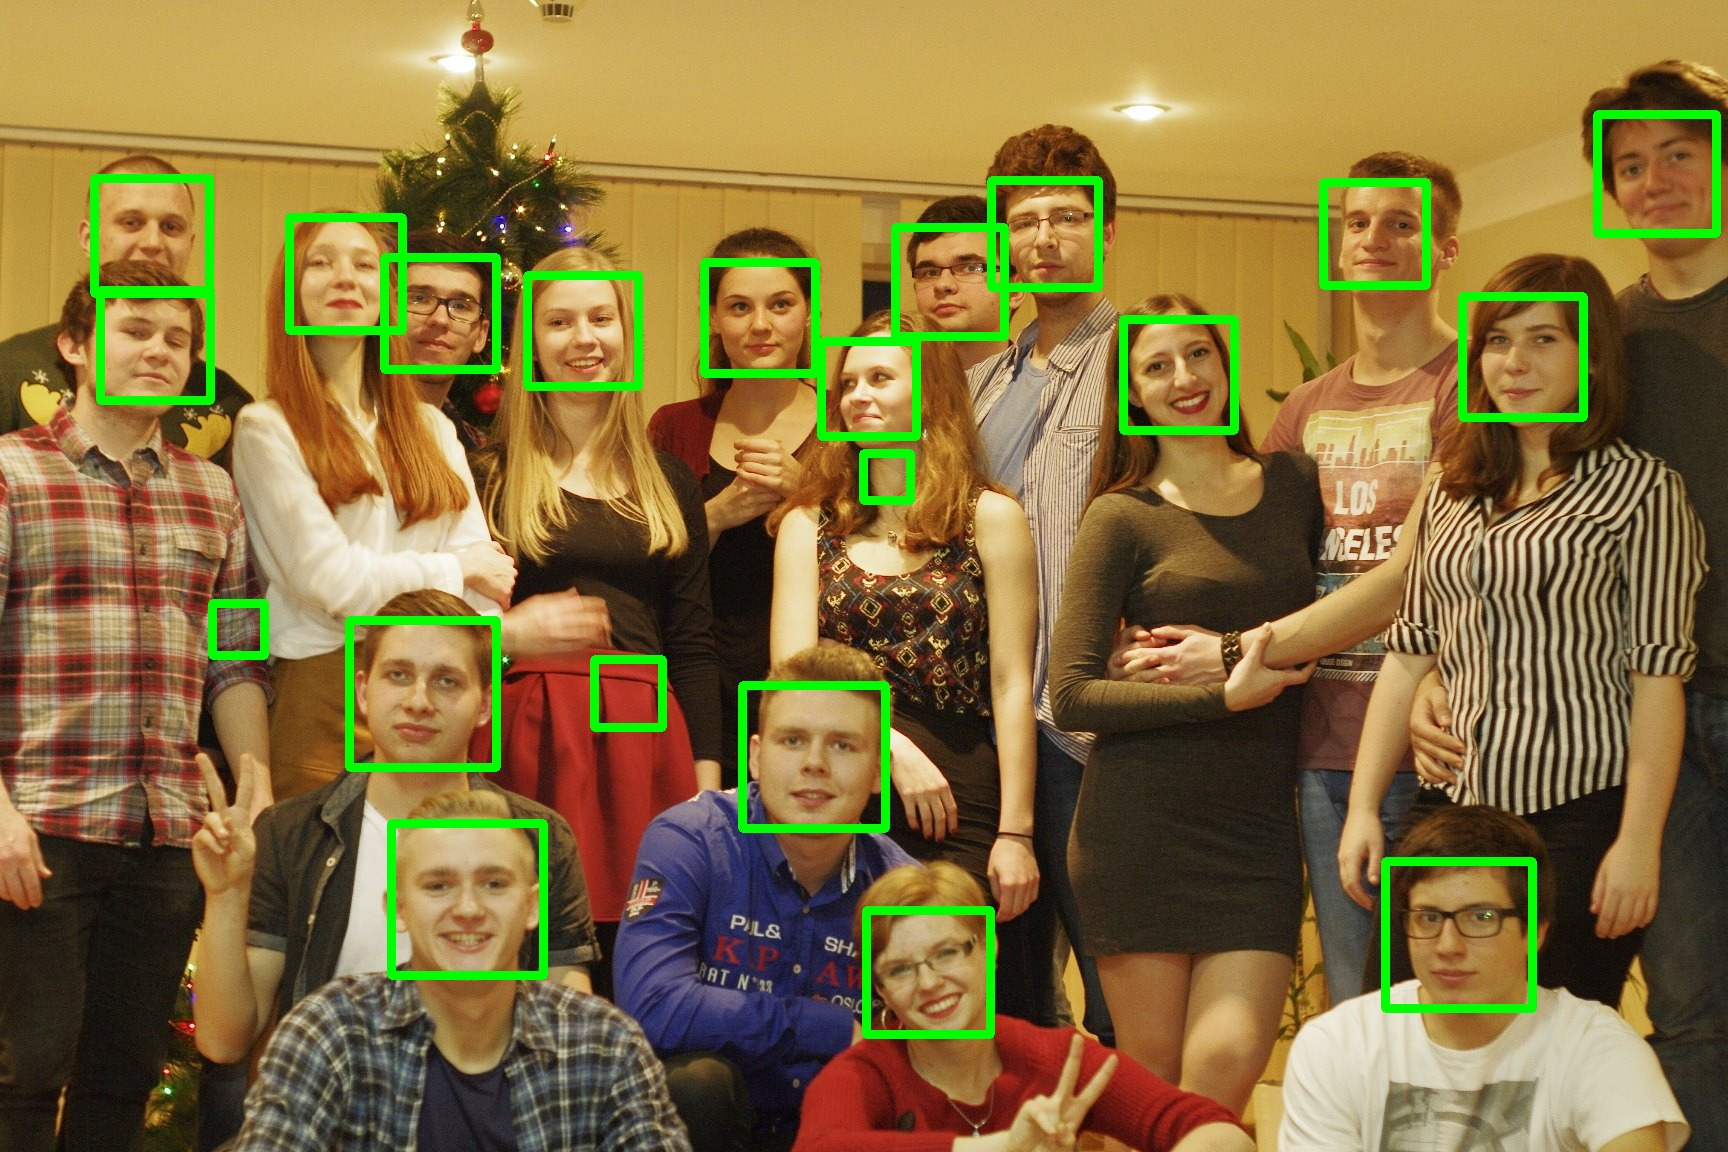
\includegraphics[width=\linewidth]{imgs/twarze11.jpg}
        \caption{skala 1.1}
        \label{fig:twarzSkala11}
    \end{subfigure}\hfill
    \begin{subfigure}{0.32\textwidth}
        \centering
        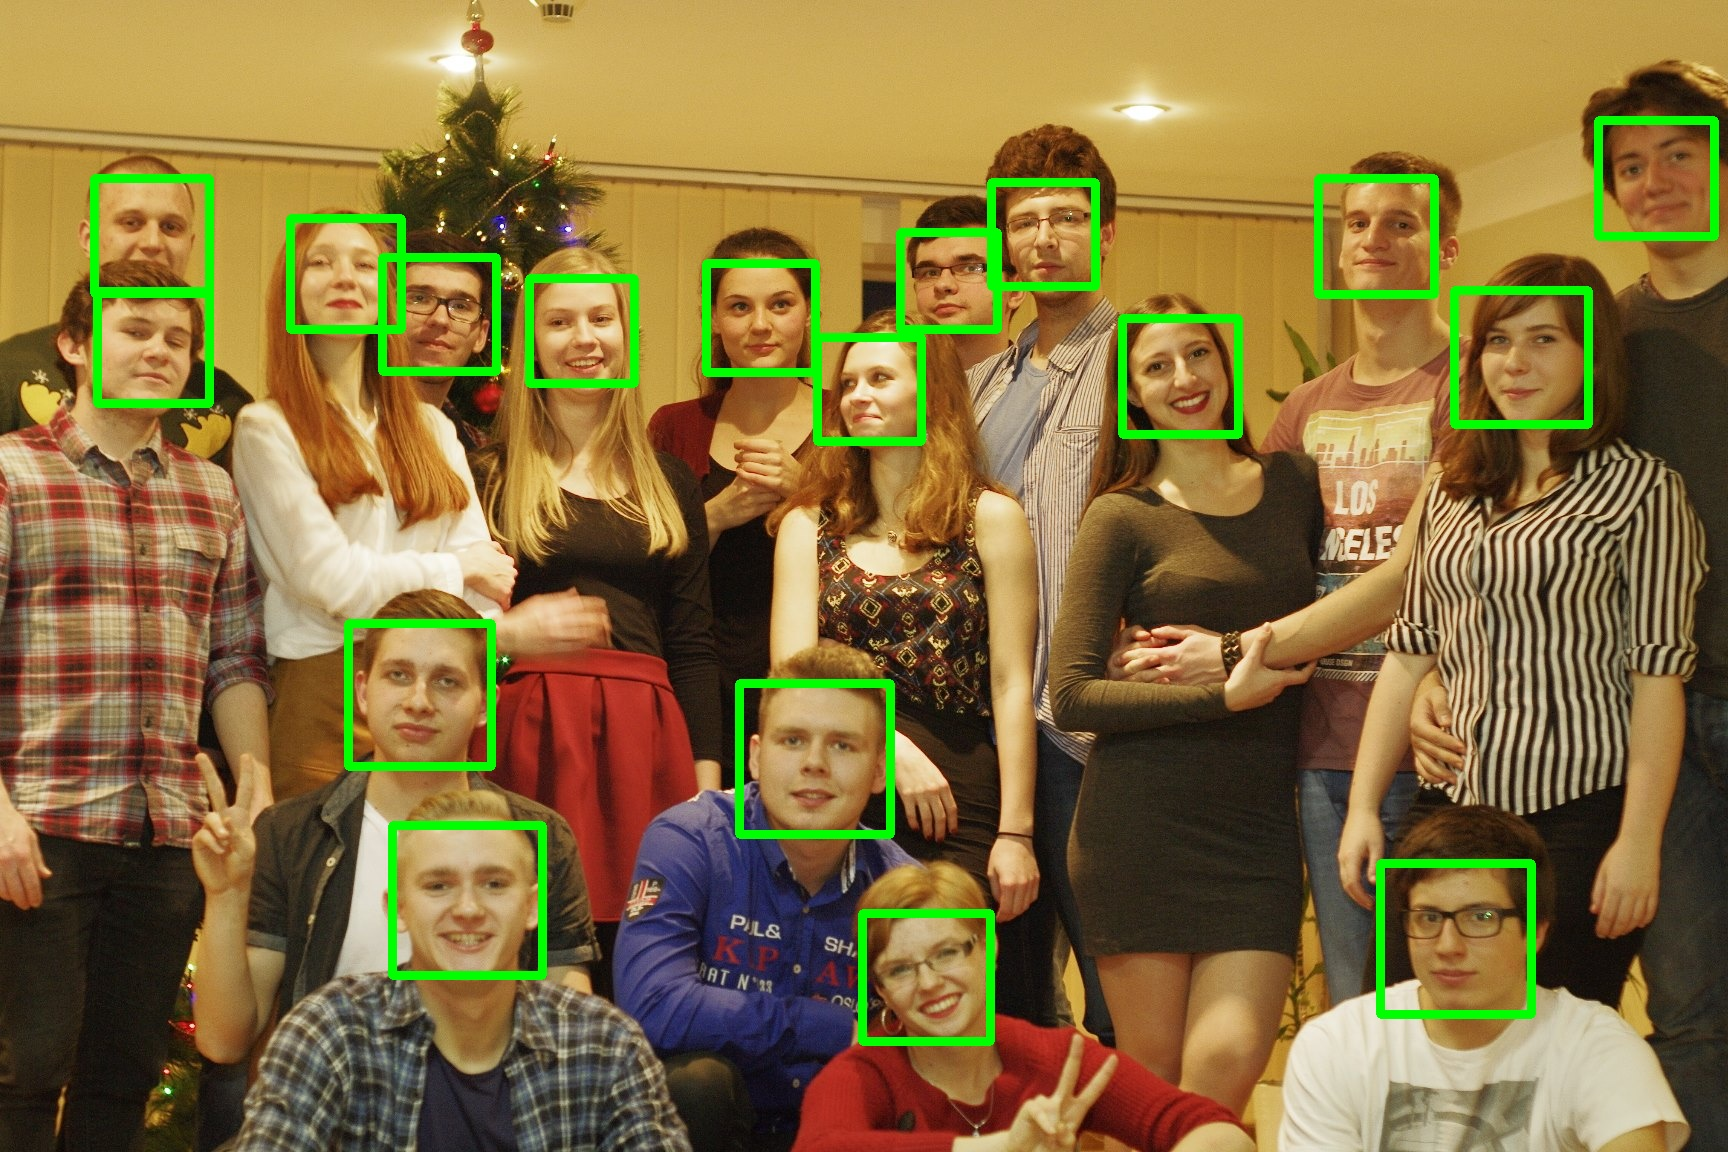
\includegraphics[width=\linewidth]{imgs/twarze13.jpg}
        \caption{skala 1.3}
        \label{fig:twarzSkala13}
    \end{subfigure}\hfill
    \begin{subfigure}{0.32\textwidth}
        \centering
        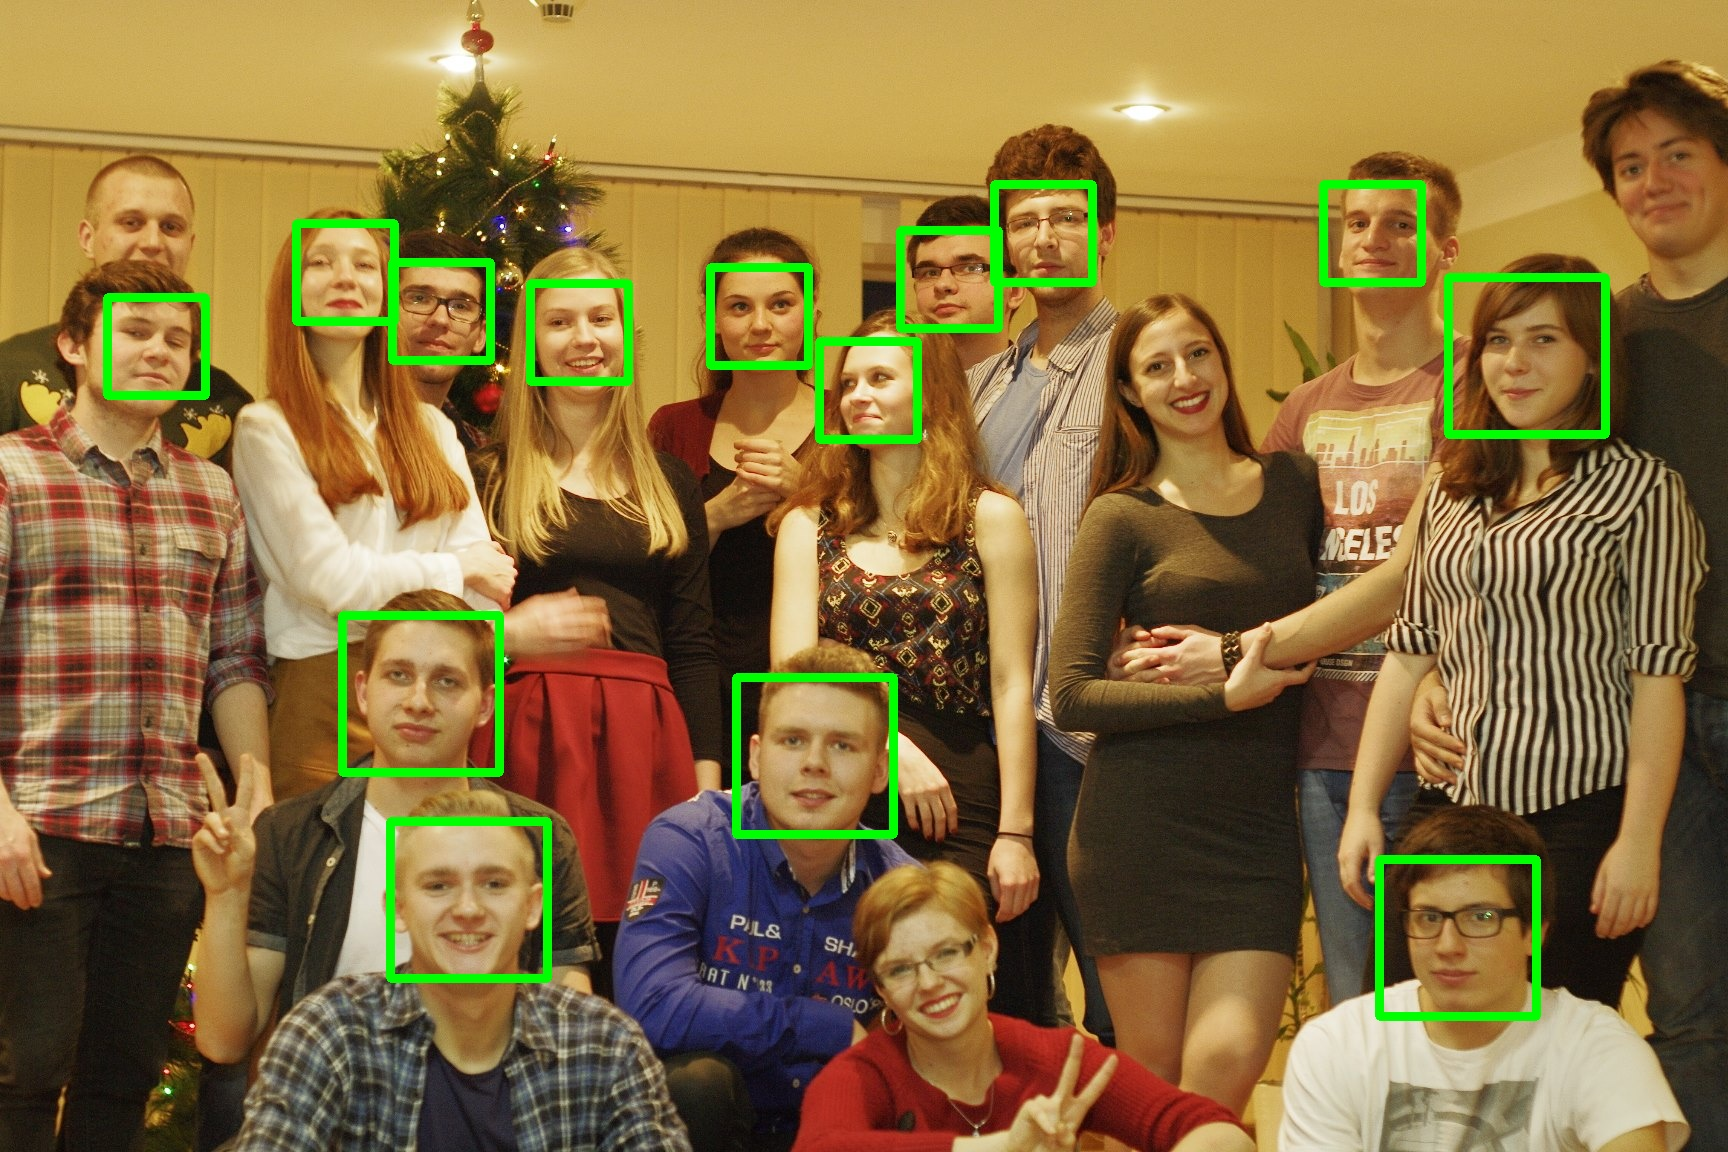
\includegraphics[width=\linewidth]{imgs/twarze16.jpg}
        \caption{skala 1.6}
        \label{fig:twarzSkala16}
    \end{subfigure}
    \caption{Detekcja twarzy dla różnych wartości scaleFactor}
    \label{twarzee}
\end{figure}

\begin{figure}[H]
    \centering
        \begin{subfigure}{0.32\textwidth}
        \centering
        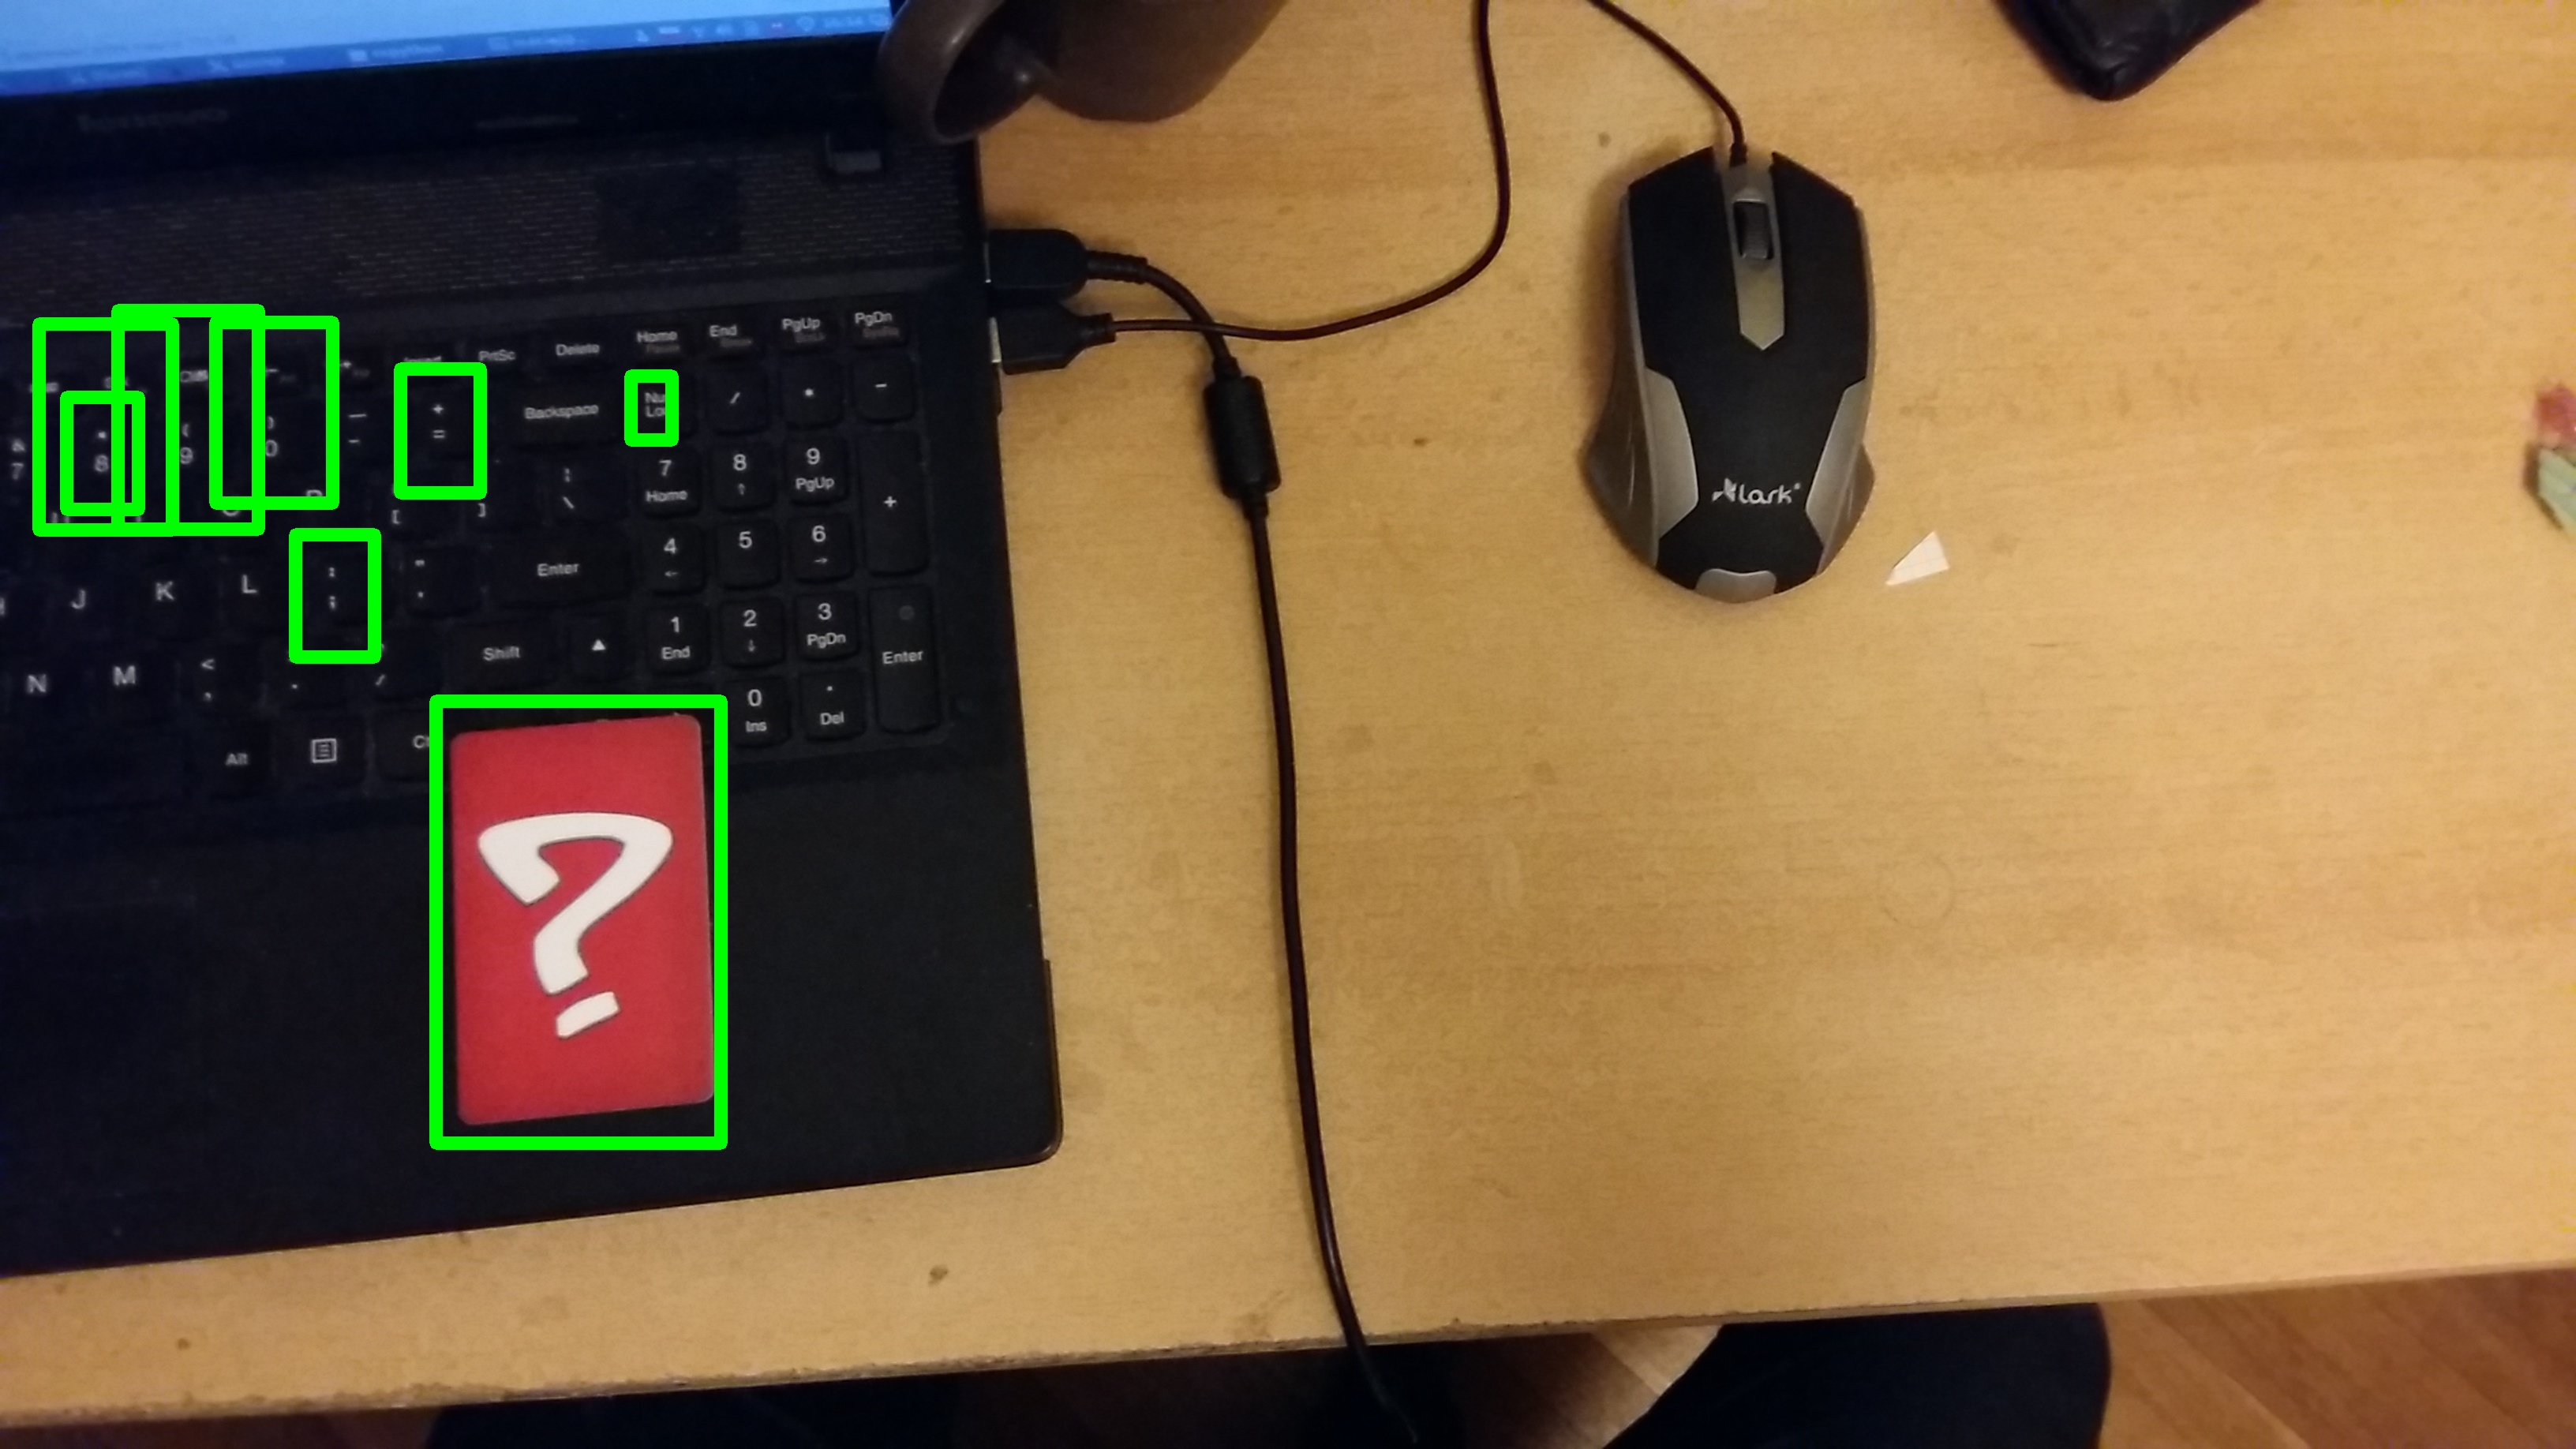
\includegraphics[width=\linewidth]{imgs/karty11.jpg}
        \caption{skala 1.1}
        \label{fig:skalaKarta11}
    \end{subfigure}\hfill
    \begin{subfigure}{0.32\textwidth}
        \centering
        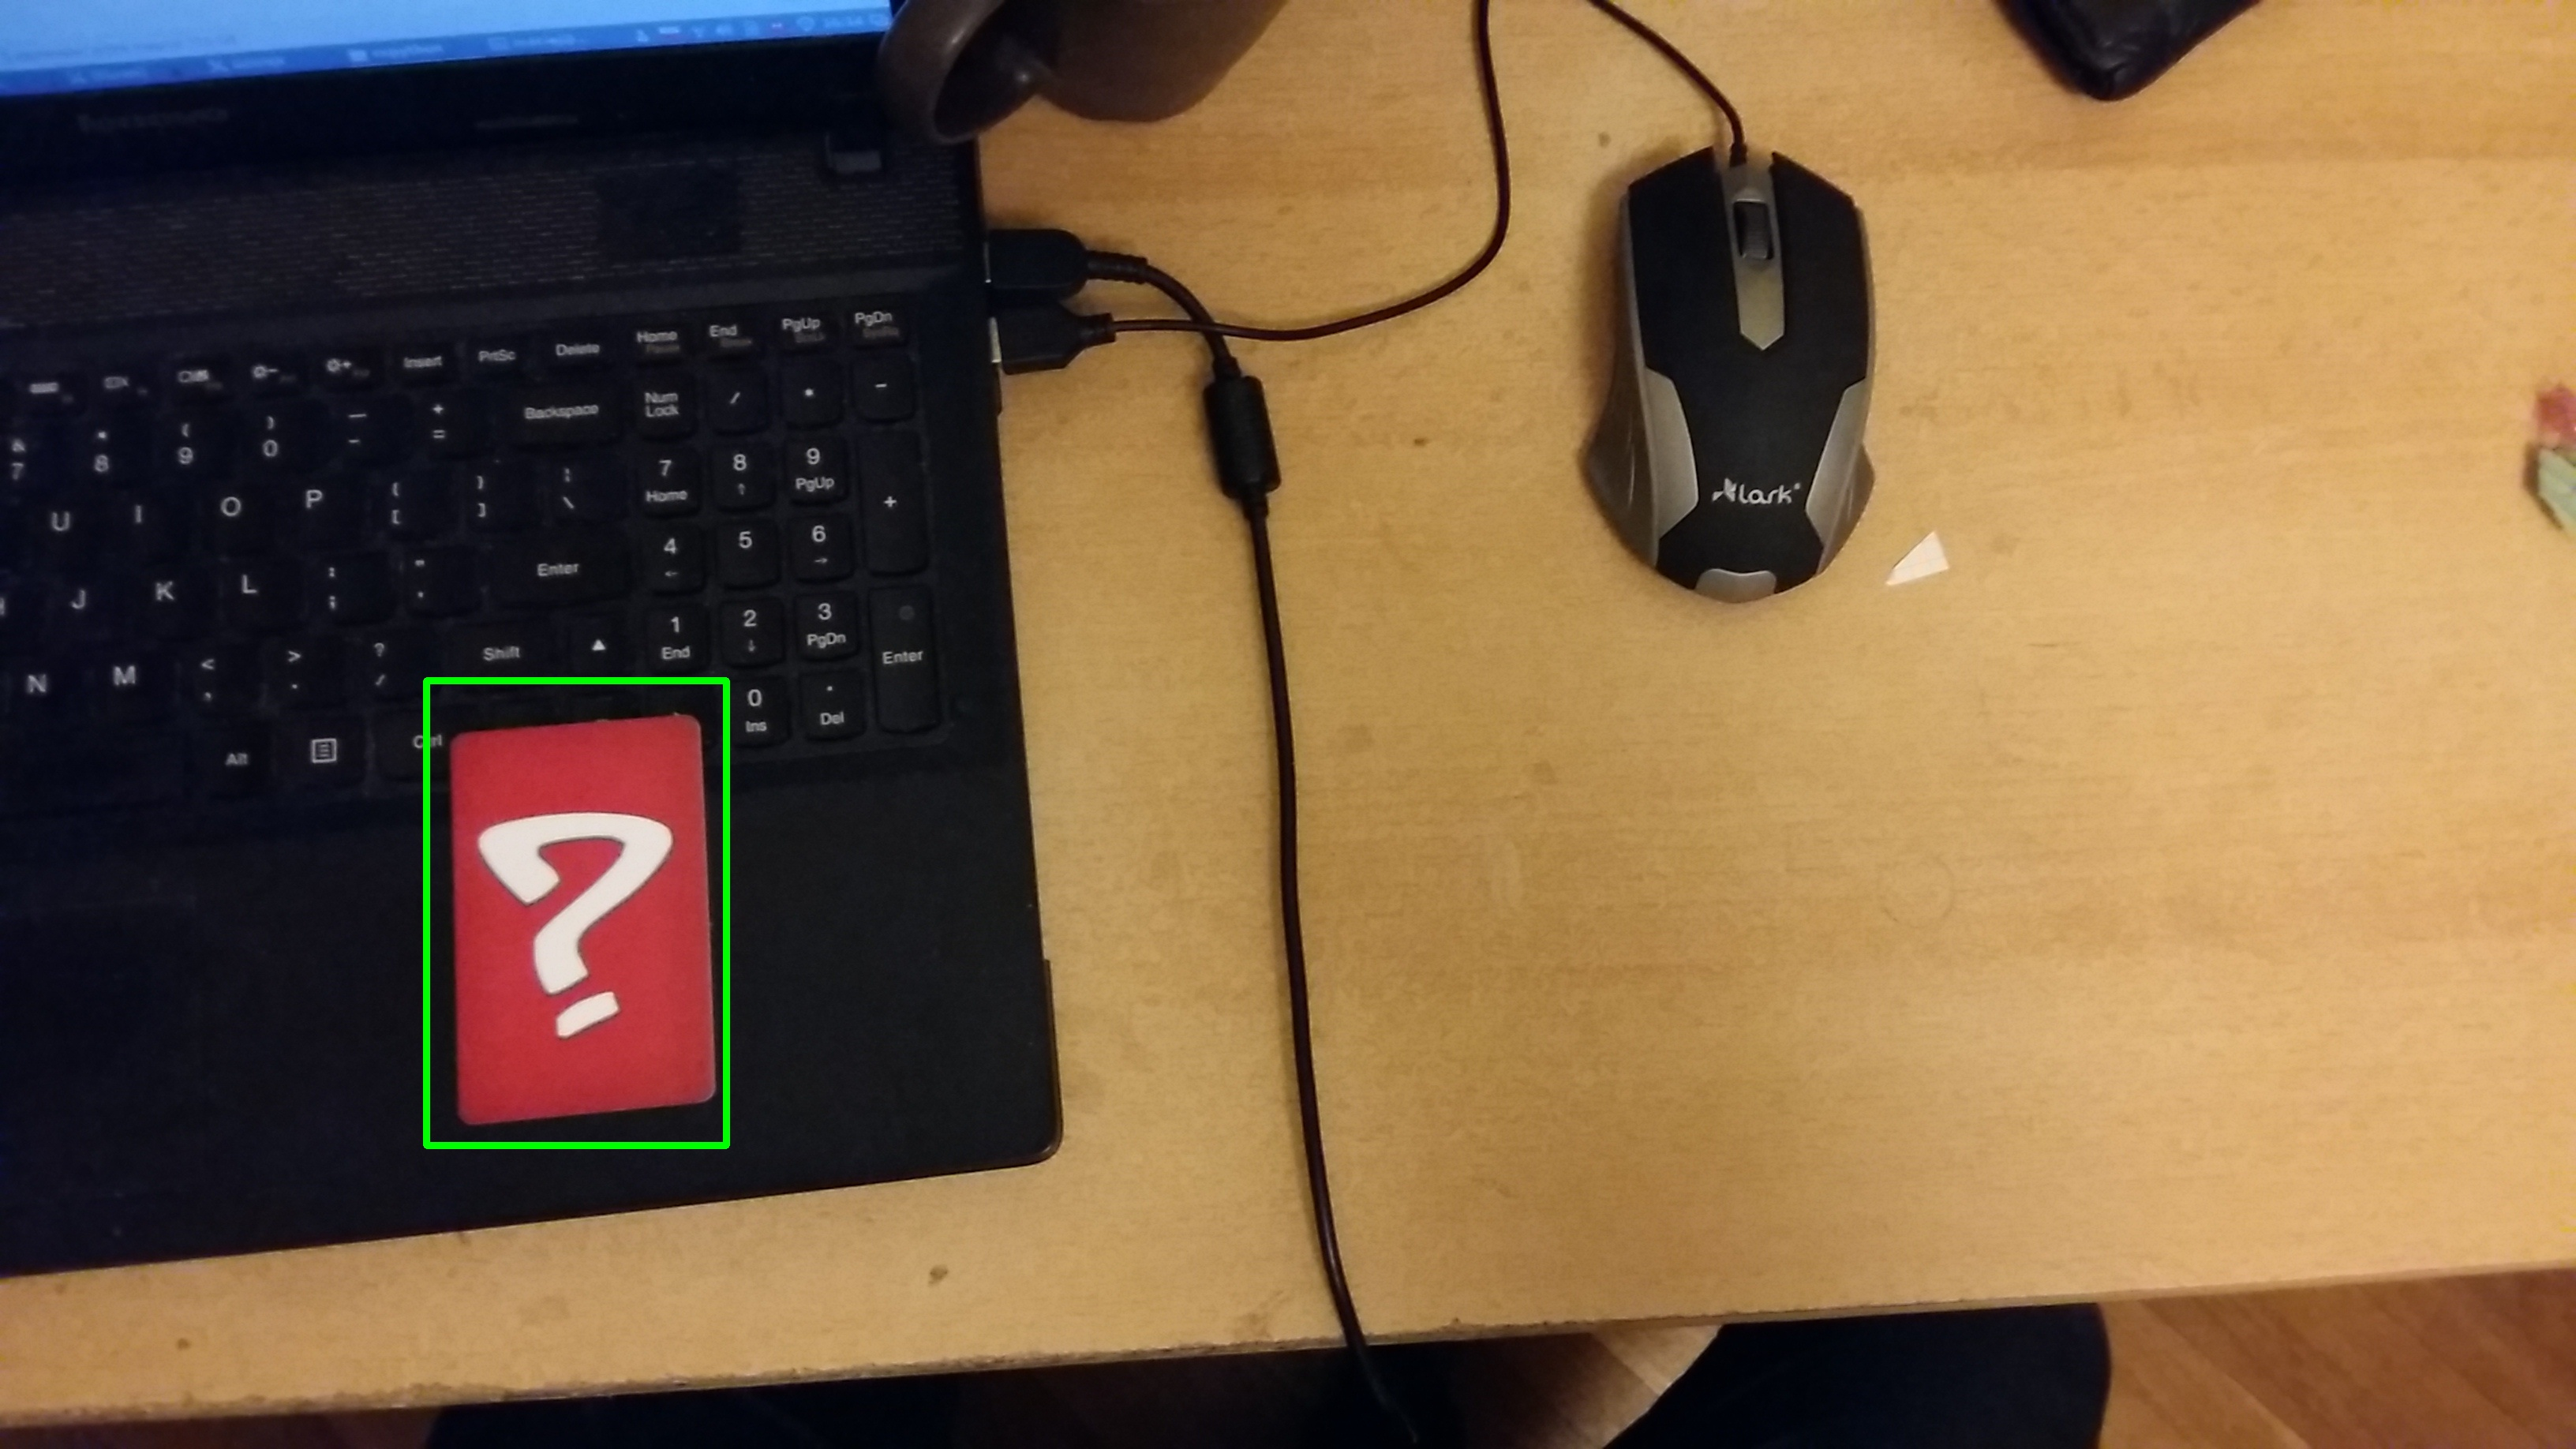
\includegraphics[width=\linewidth]{imgs/karta13.jpg}
        \caption{skala 1.3}
        \label{fig:skalaKarta13}
    \end{subfigure}\hfill
    \begin{subfigure}{0.32\textwidth}
        \centering
        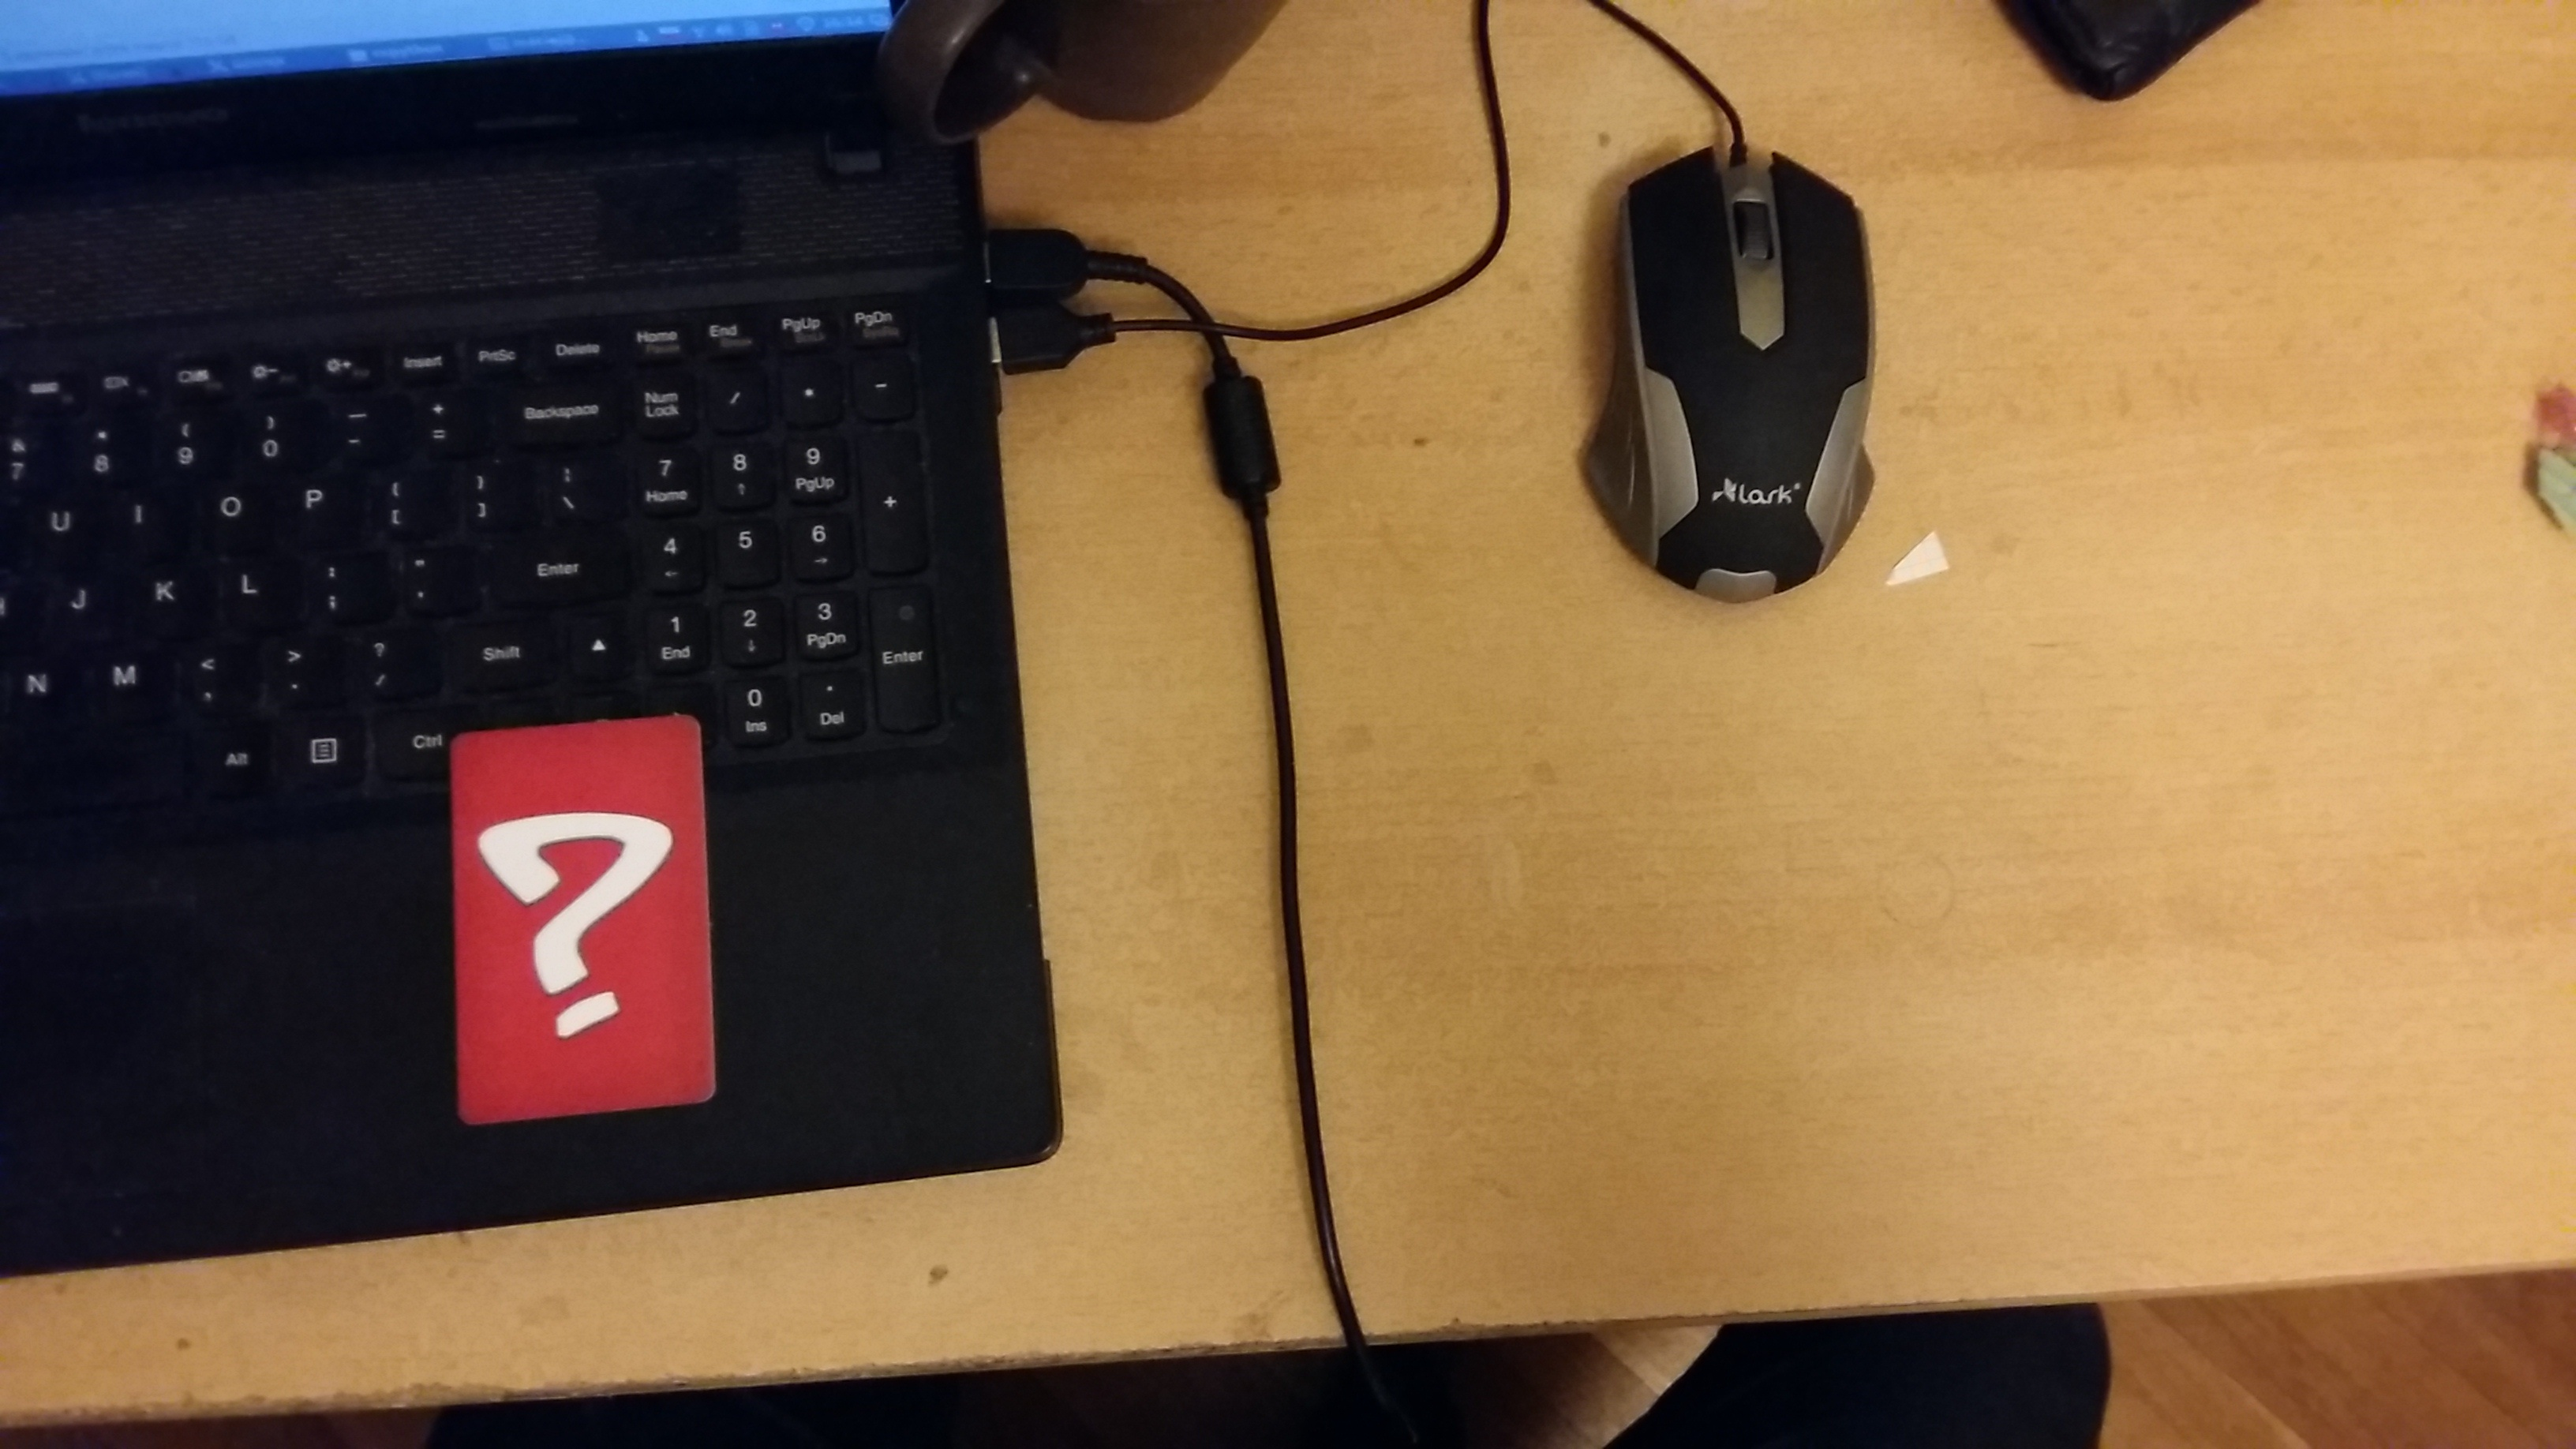
\includegraphics[width=\linewidth]{imgs/kartaaskala20.jpg}
        \caption{skala 2.0}
        \label{fig:skalaKarta20}
    \end{subfigure}
    \caption{Detekcja karty dla różnych wartości scaleFactor}
    \label{kartyy}
\end{figure}

\begin{table}[H]
    \caption{Wyniki detekcji w zalezności od parametru scaleFactor}
    \label{tab:skale}
    \begin{tabular}{|l|c|c|c|c|c|c|c|}
\hline
Rysunek & \ref{fig:twarzSkala11} & \ref{fig:twarzSkala13} & \ref{fig:twarzSkala16} & \ref{fig:skalaKarta11} & \ref{fig:skalaKarta13} & \ref{fig:skalaKarta20}\\
\hline
Skala & 1.1 & 1.3 & 1.6 & 1.1 & 1.3 & 2.0\\
\hline
Czas & 379,397 & 161,874 & 105,139 & 475,516 & 215,779 & 108,829\\
\hline
$F_{pos}$ & 3 & 0 & 0 & 7 & 0 & 0\\
\hline
$F_{neg}$ & 0 & 0 & 3 & 0 & 0 & 1\\
\hline
\end{tabular}
\end{table}

Rysunki \ref{twarzee} i \ref{kartyy} przedstawiają wyniki detekcji twarzy oraz karty dla różnych parametrów scaleFactor. W tabeli \ref{tab:skale} przedstawiono czas detekcji, liczbę błędnych klasyfikacji jako obiekt oznaczonych jako ${F_{pos}}$ oraz liczbę błędnych klasyfikacji jako nie obiekt ${F_{neg}}$ Jak widać im mniejszy parametr tym czas krótszy, ${F_{pos}}$ także się zmniejsza natomiast rośnie wartość ${F_{neg}}$.

Parametr minNeighbors określa w ilu sąsiednich ramkach został odnaleziony obiekt, dopiero przy odpowiedniej liczbie tych sąsiadów podejmowana jest decyzja o znalezieniu wzoru. Zwiększanie tego współczynnika zmniejsza prawdopodobieństwo podjęcia błędnej decyzji o poprawnej detekcji, natomiast zwiększa ryzyko pominięcia elementu.


\begin{figure}[H]
    \centering
        \begin{subfigure}{0.32\textwidth}
        \centering
        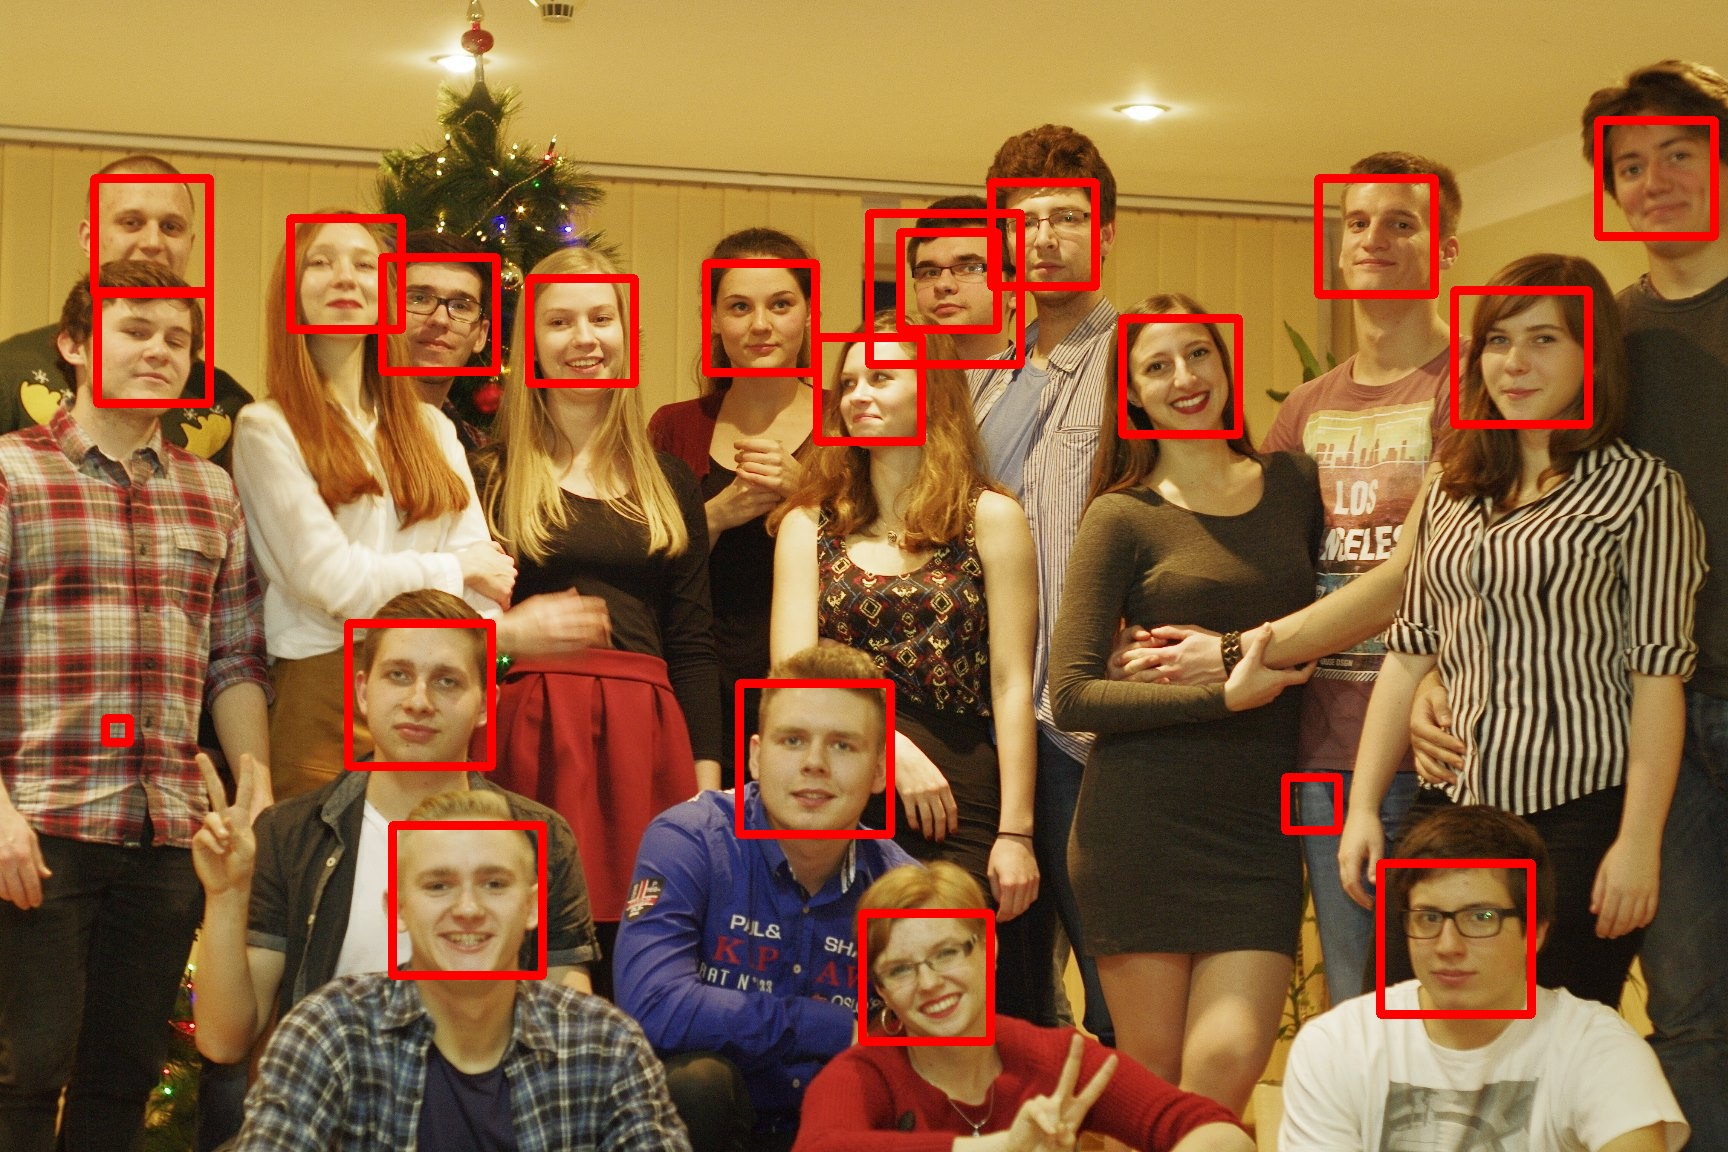
\includegraphics[width=\linewidth]{imgs/somsiad1.jpg}
        \caption{minNeighbors równe 1}
        \label{fig:somsiadTwarze1}
    \end{subfigure}\hfill
    \begin{subfigure}{0.32\textwidth}
        \centering
        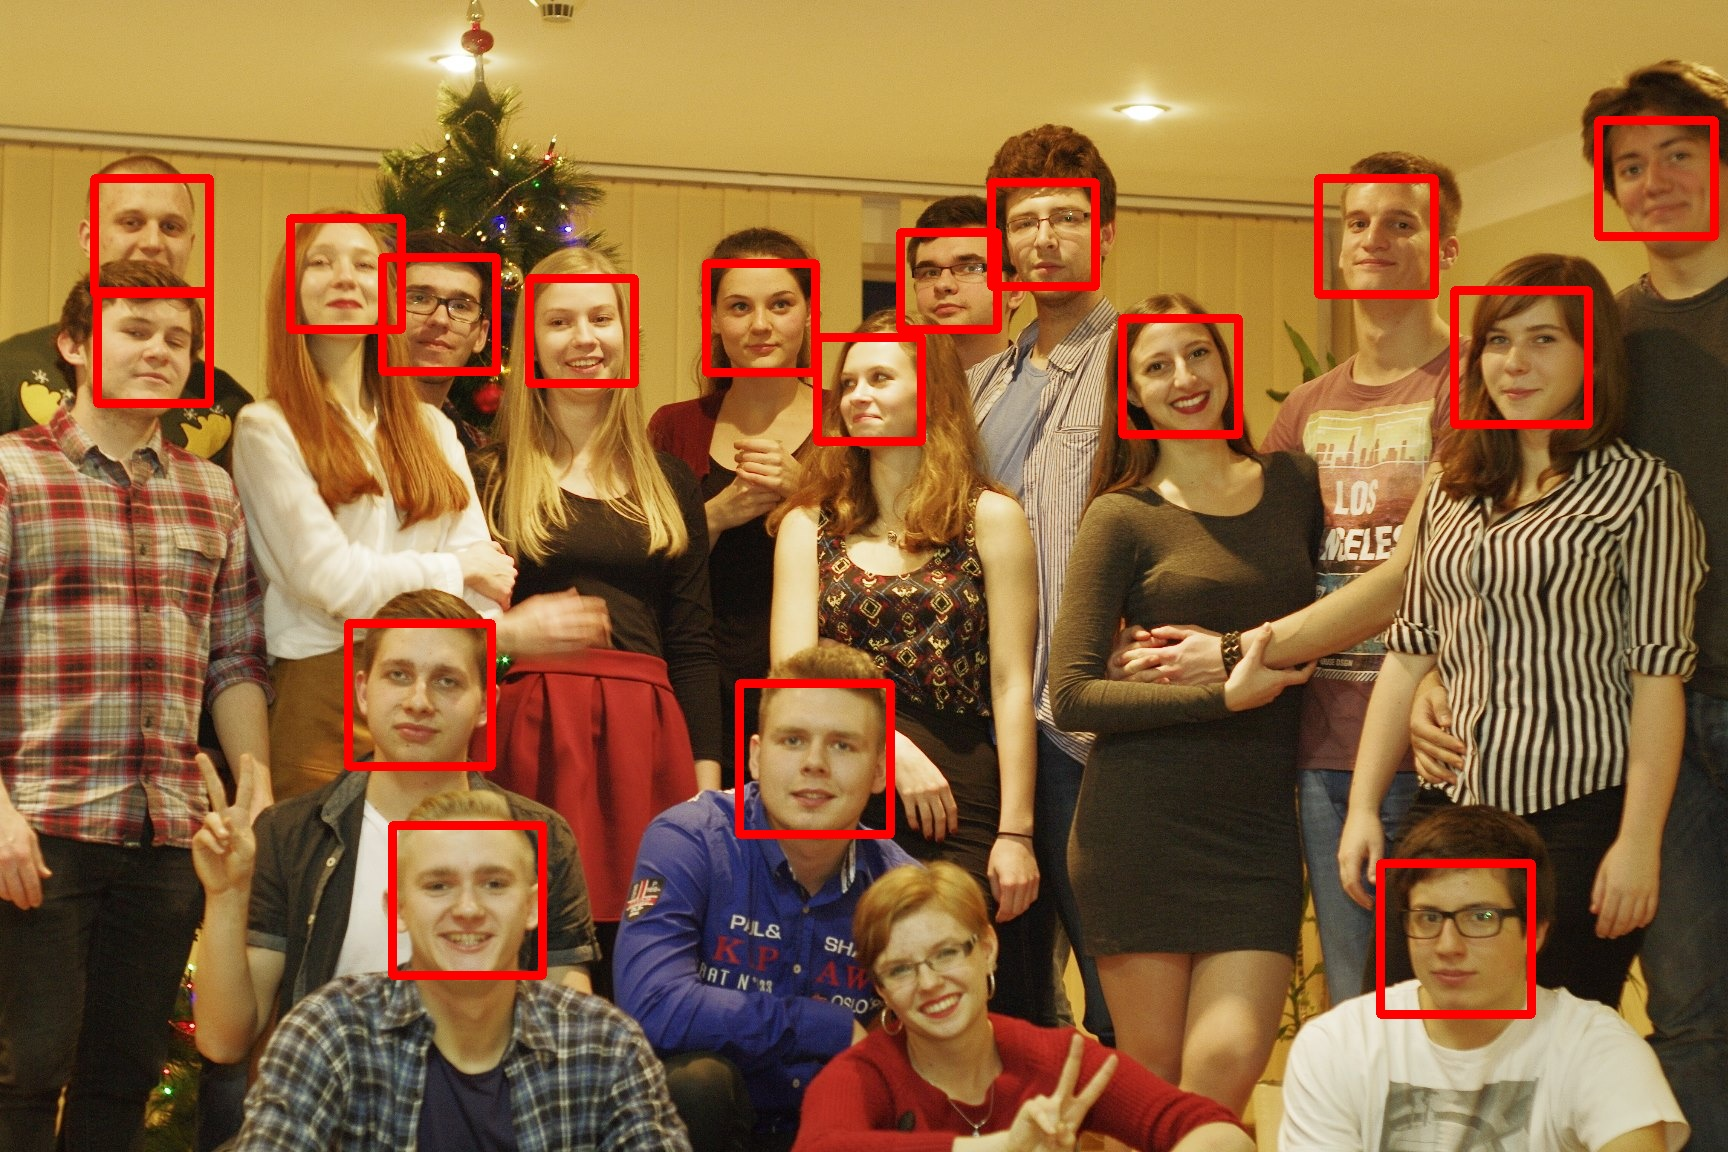
\includegraphics[width=\linewidth]{imgs/somsiad3.jpg}
        \caption{minNeighbors równe 3}
        \label{fig:somsiadTwarze3}
    \end{subfigure}\hfill
    \begin{subfigure}{0.32\textwidth}
        \centering
        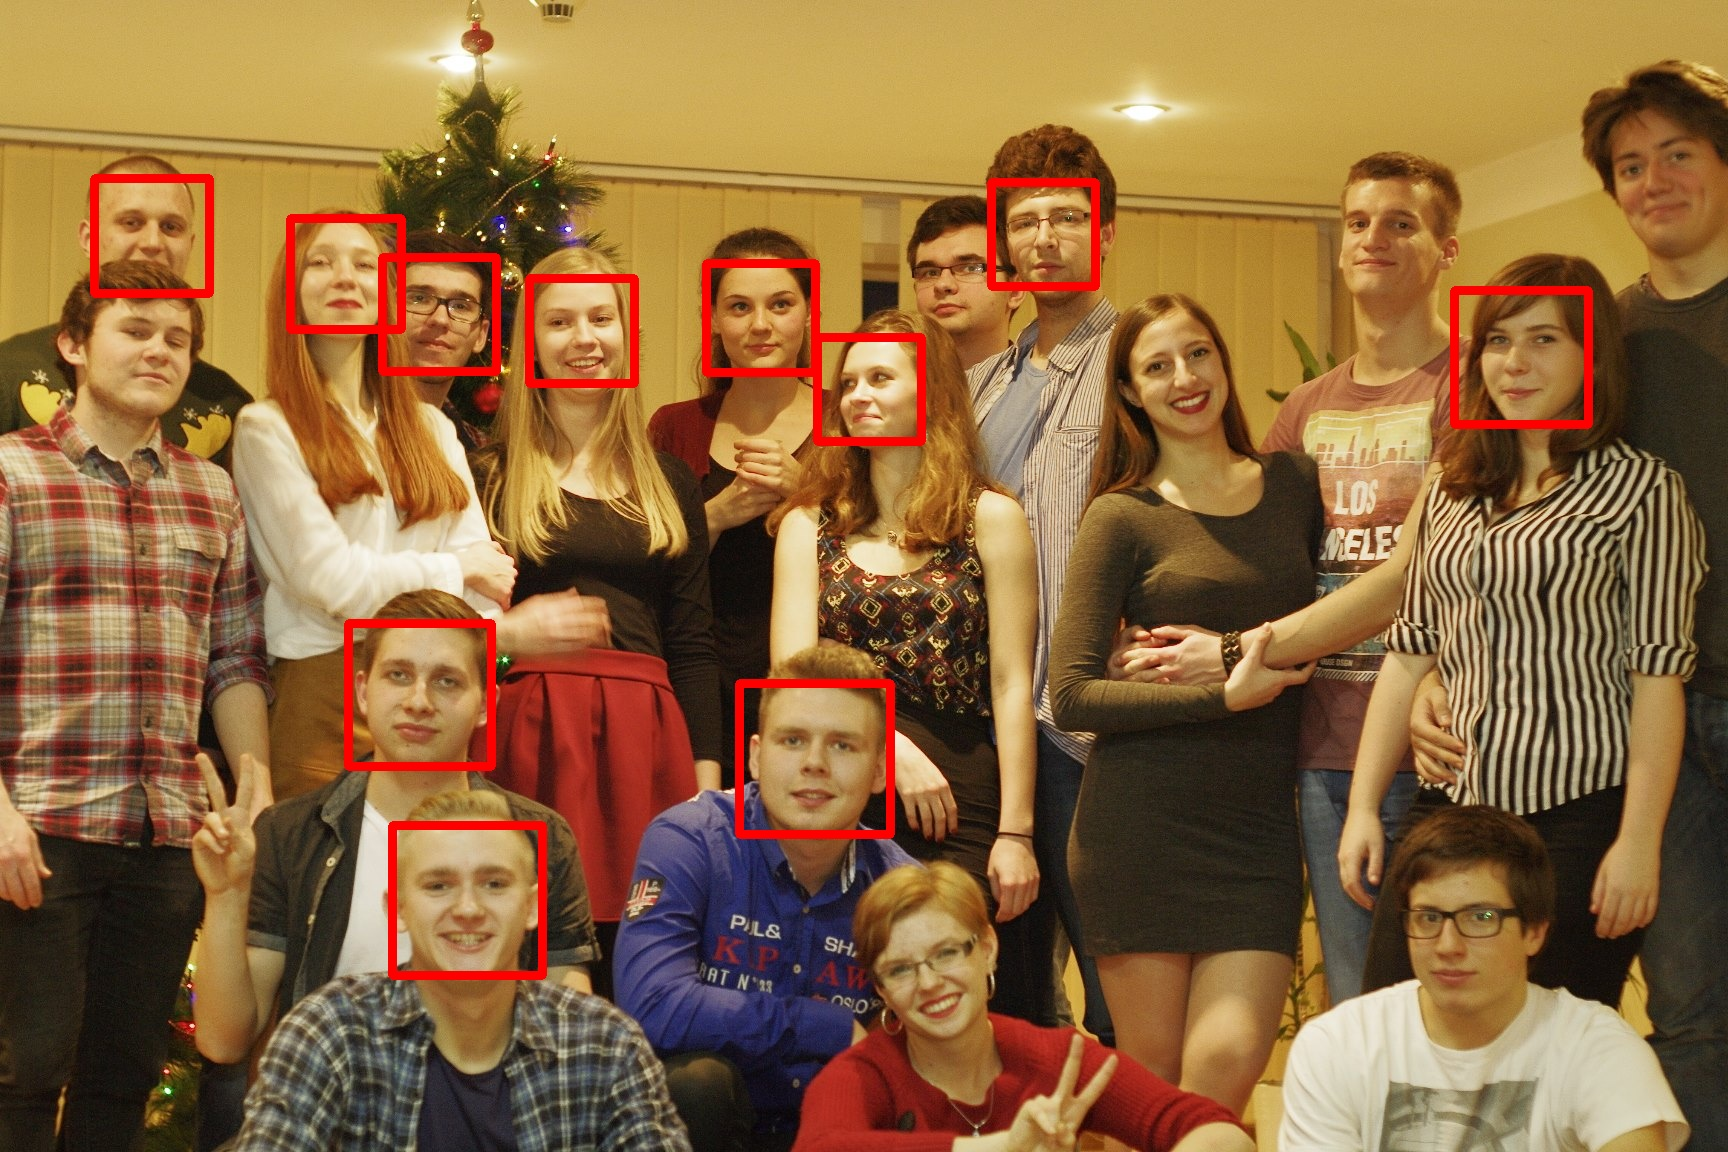
\includegraphics[width=\linewidth]{imgs/somsiad8.jpg}
        \caption{minNeighbors równe 8}
        \label{fig:somsiadTwarze8}
    \end{subfigure}
    \caption{Detekcja twarzy dla różnych wartości minNeighbors}
    \label{twarzeeSomsiady}
\end{figure}

\begin{figure}[H]
    \centering
        \begin{subfigure}{0.32\textwidth}
        \centering
        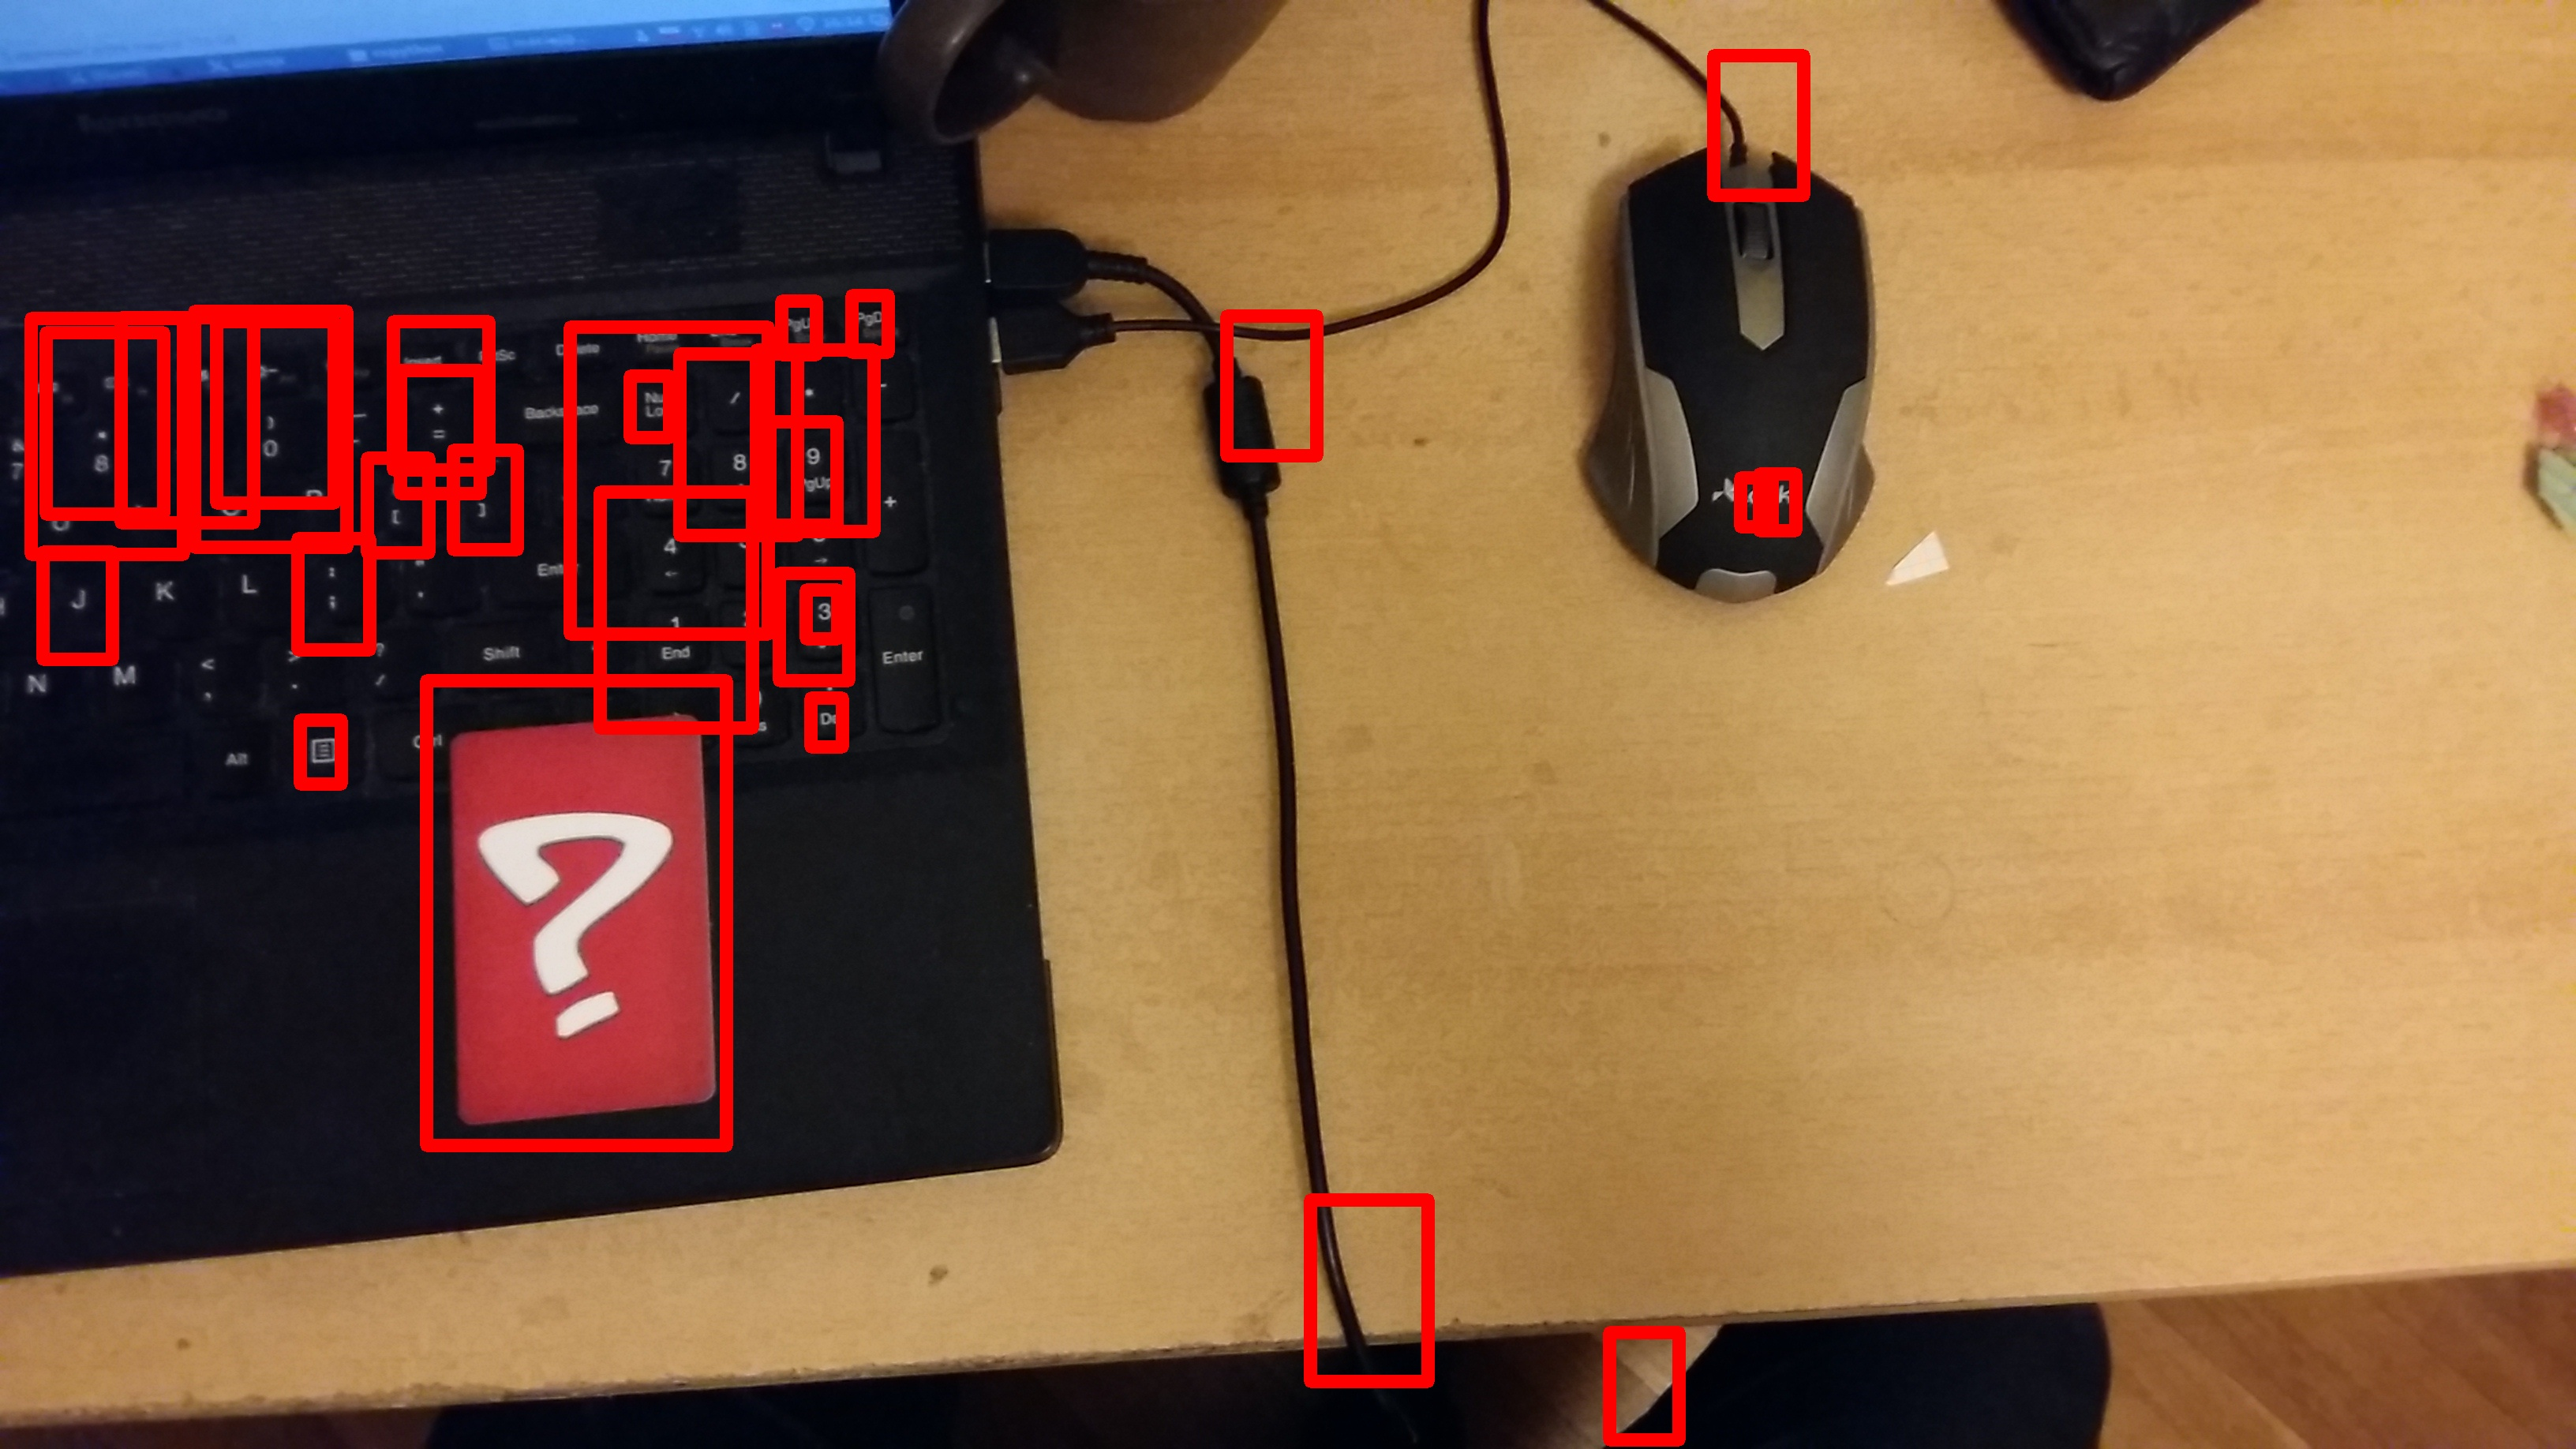
\includegraphics[width=\linewidth]{imgs/somsiadd1.jpg}
        \caption{minNeighbors równe 1}
        \label{fig:somsiadKarta1}
    \end{subfigure}\hfill
    \begin{subfigure}{0.32\textwidth}
        \centering
        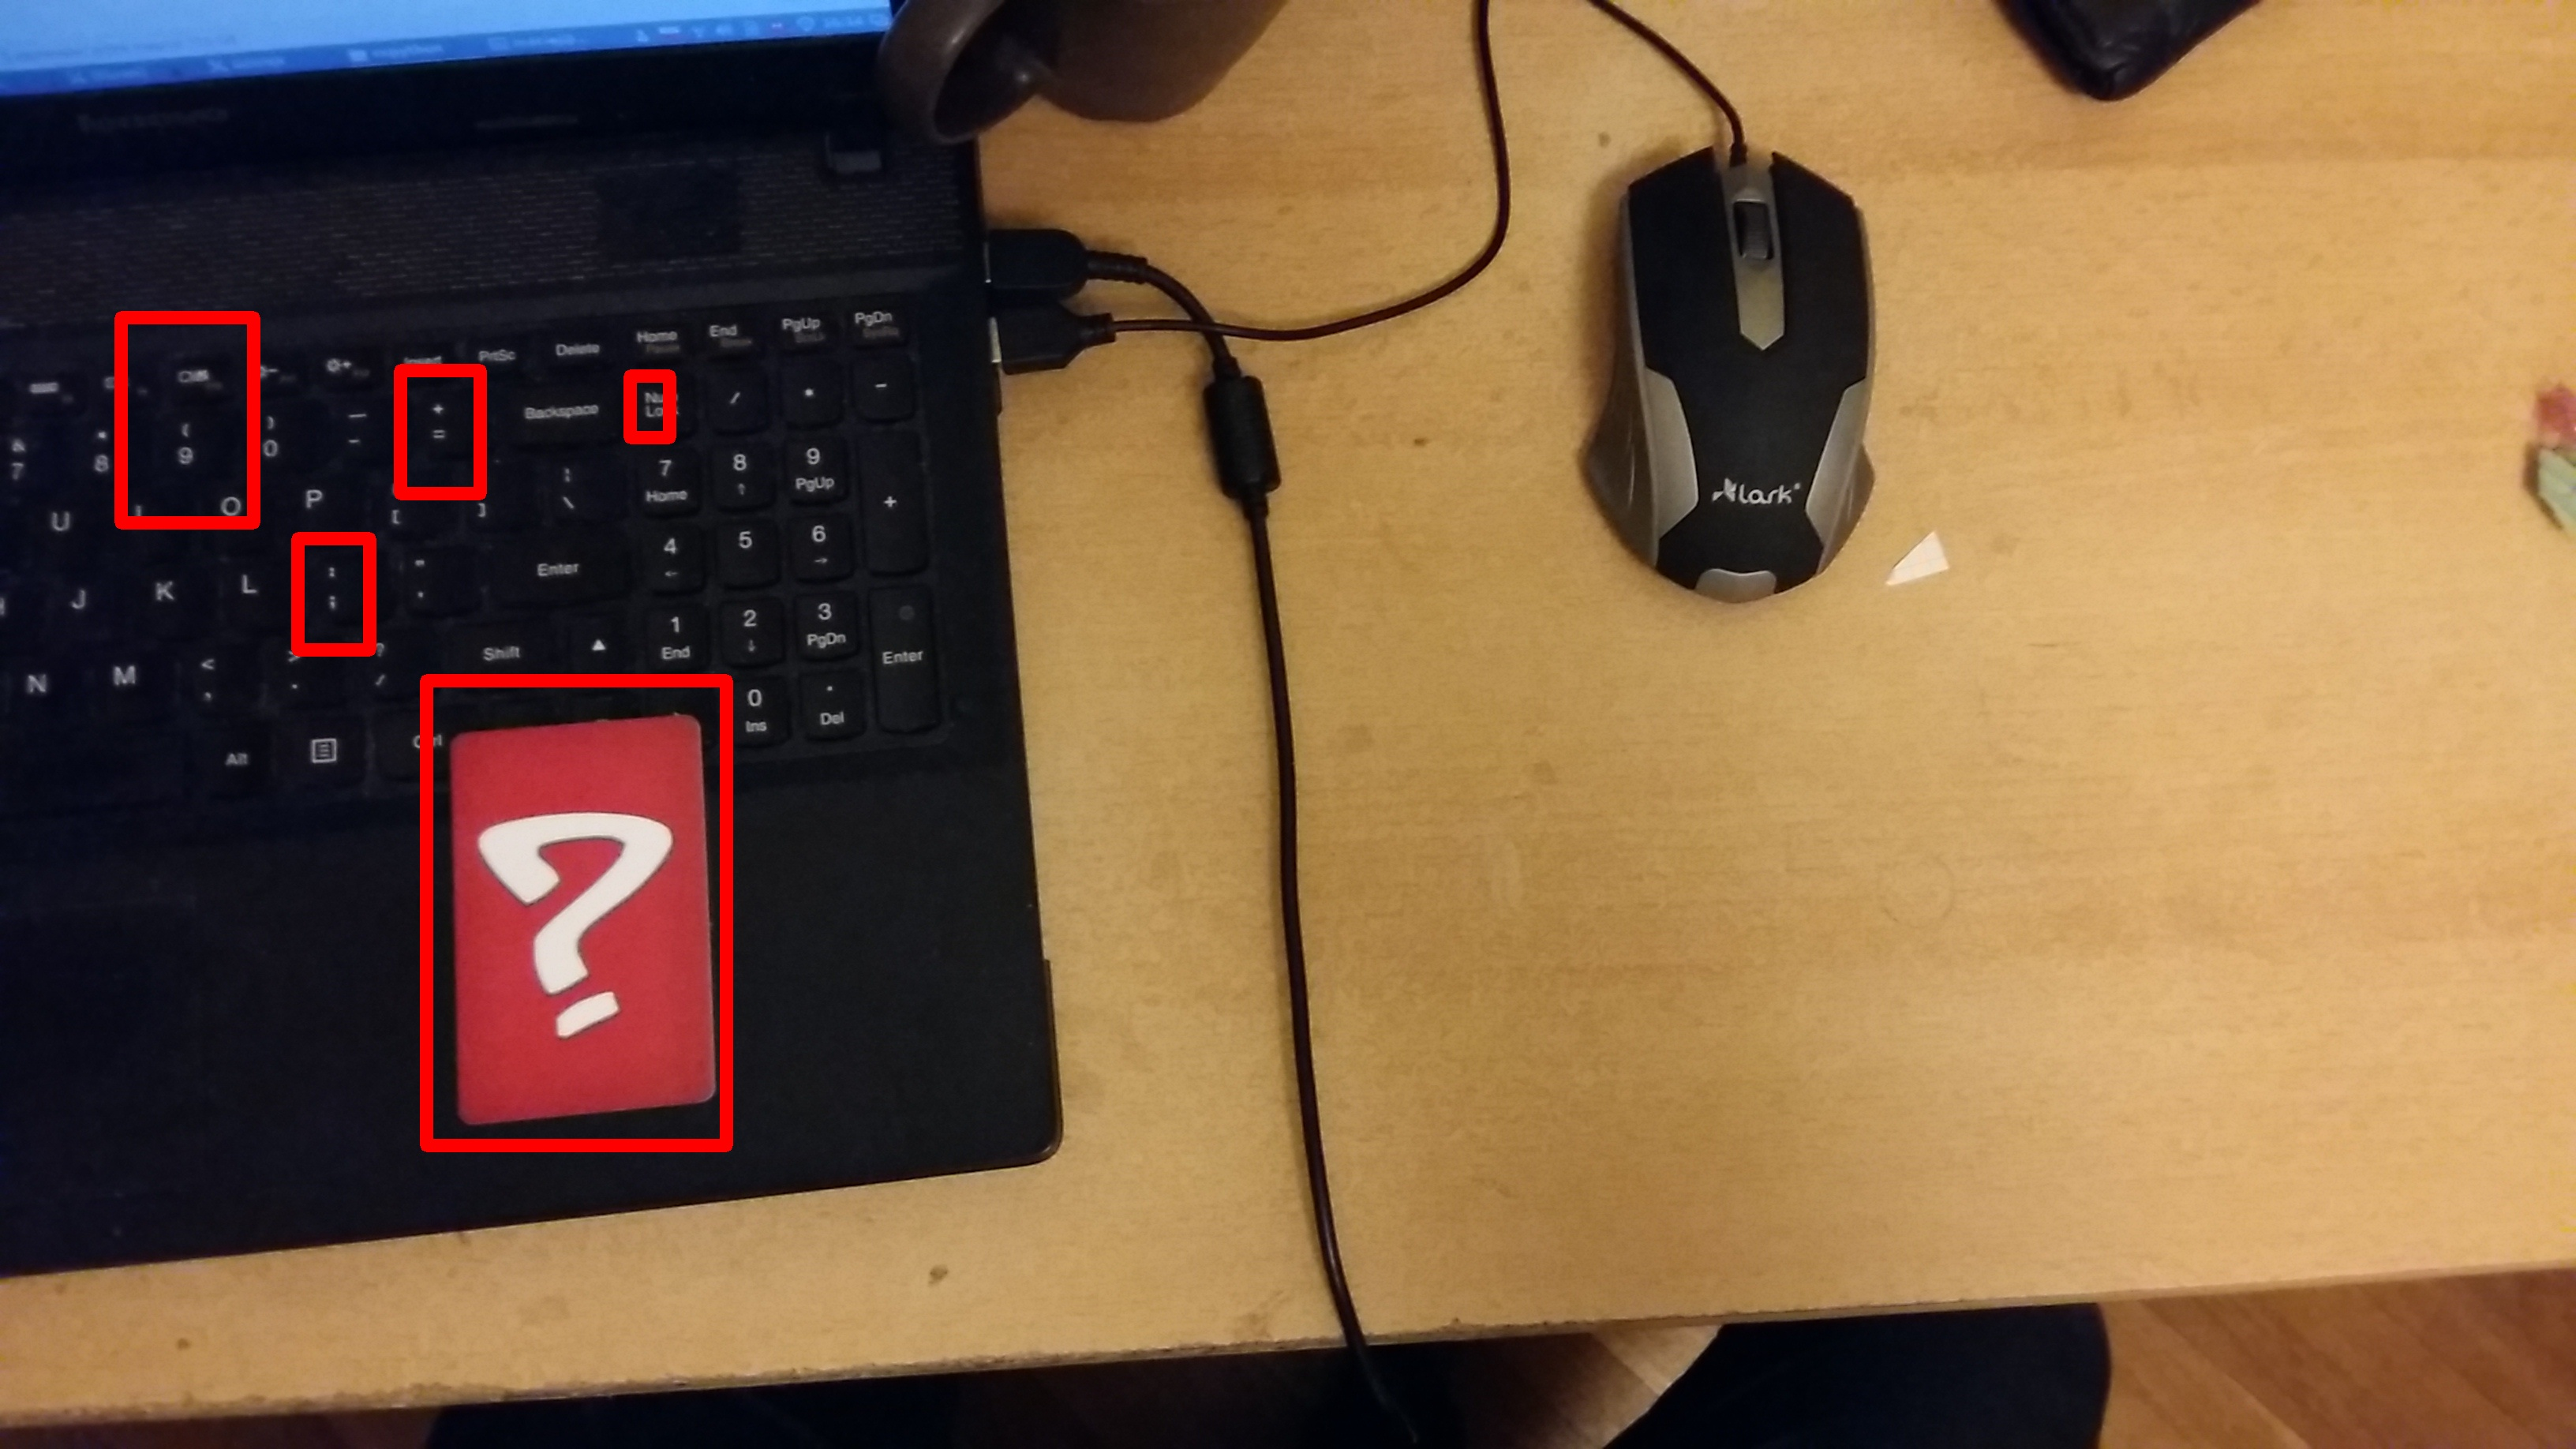
\includegraphics[width=\linewidth]{imgs/somsiadd6.jpg}
        \caption{minNeighbors równe 6}
        \label{fig:somsiadKarta6}
    \end{subfigure}\hfill
    \begin{subfigure}{0.32\textwidth}
        \centering
        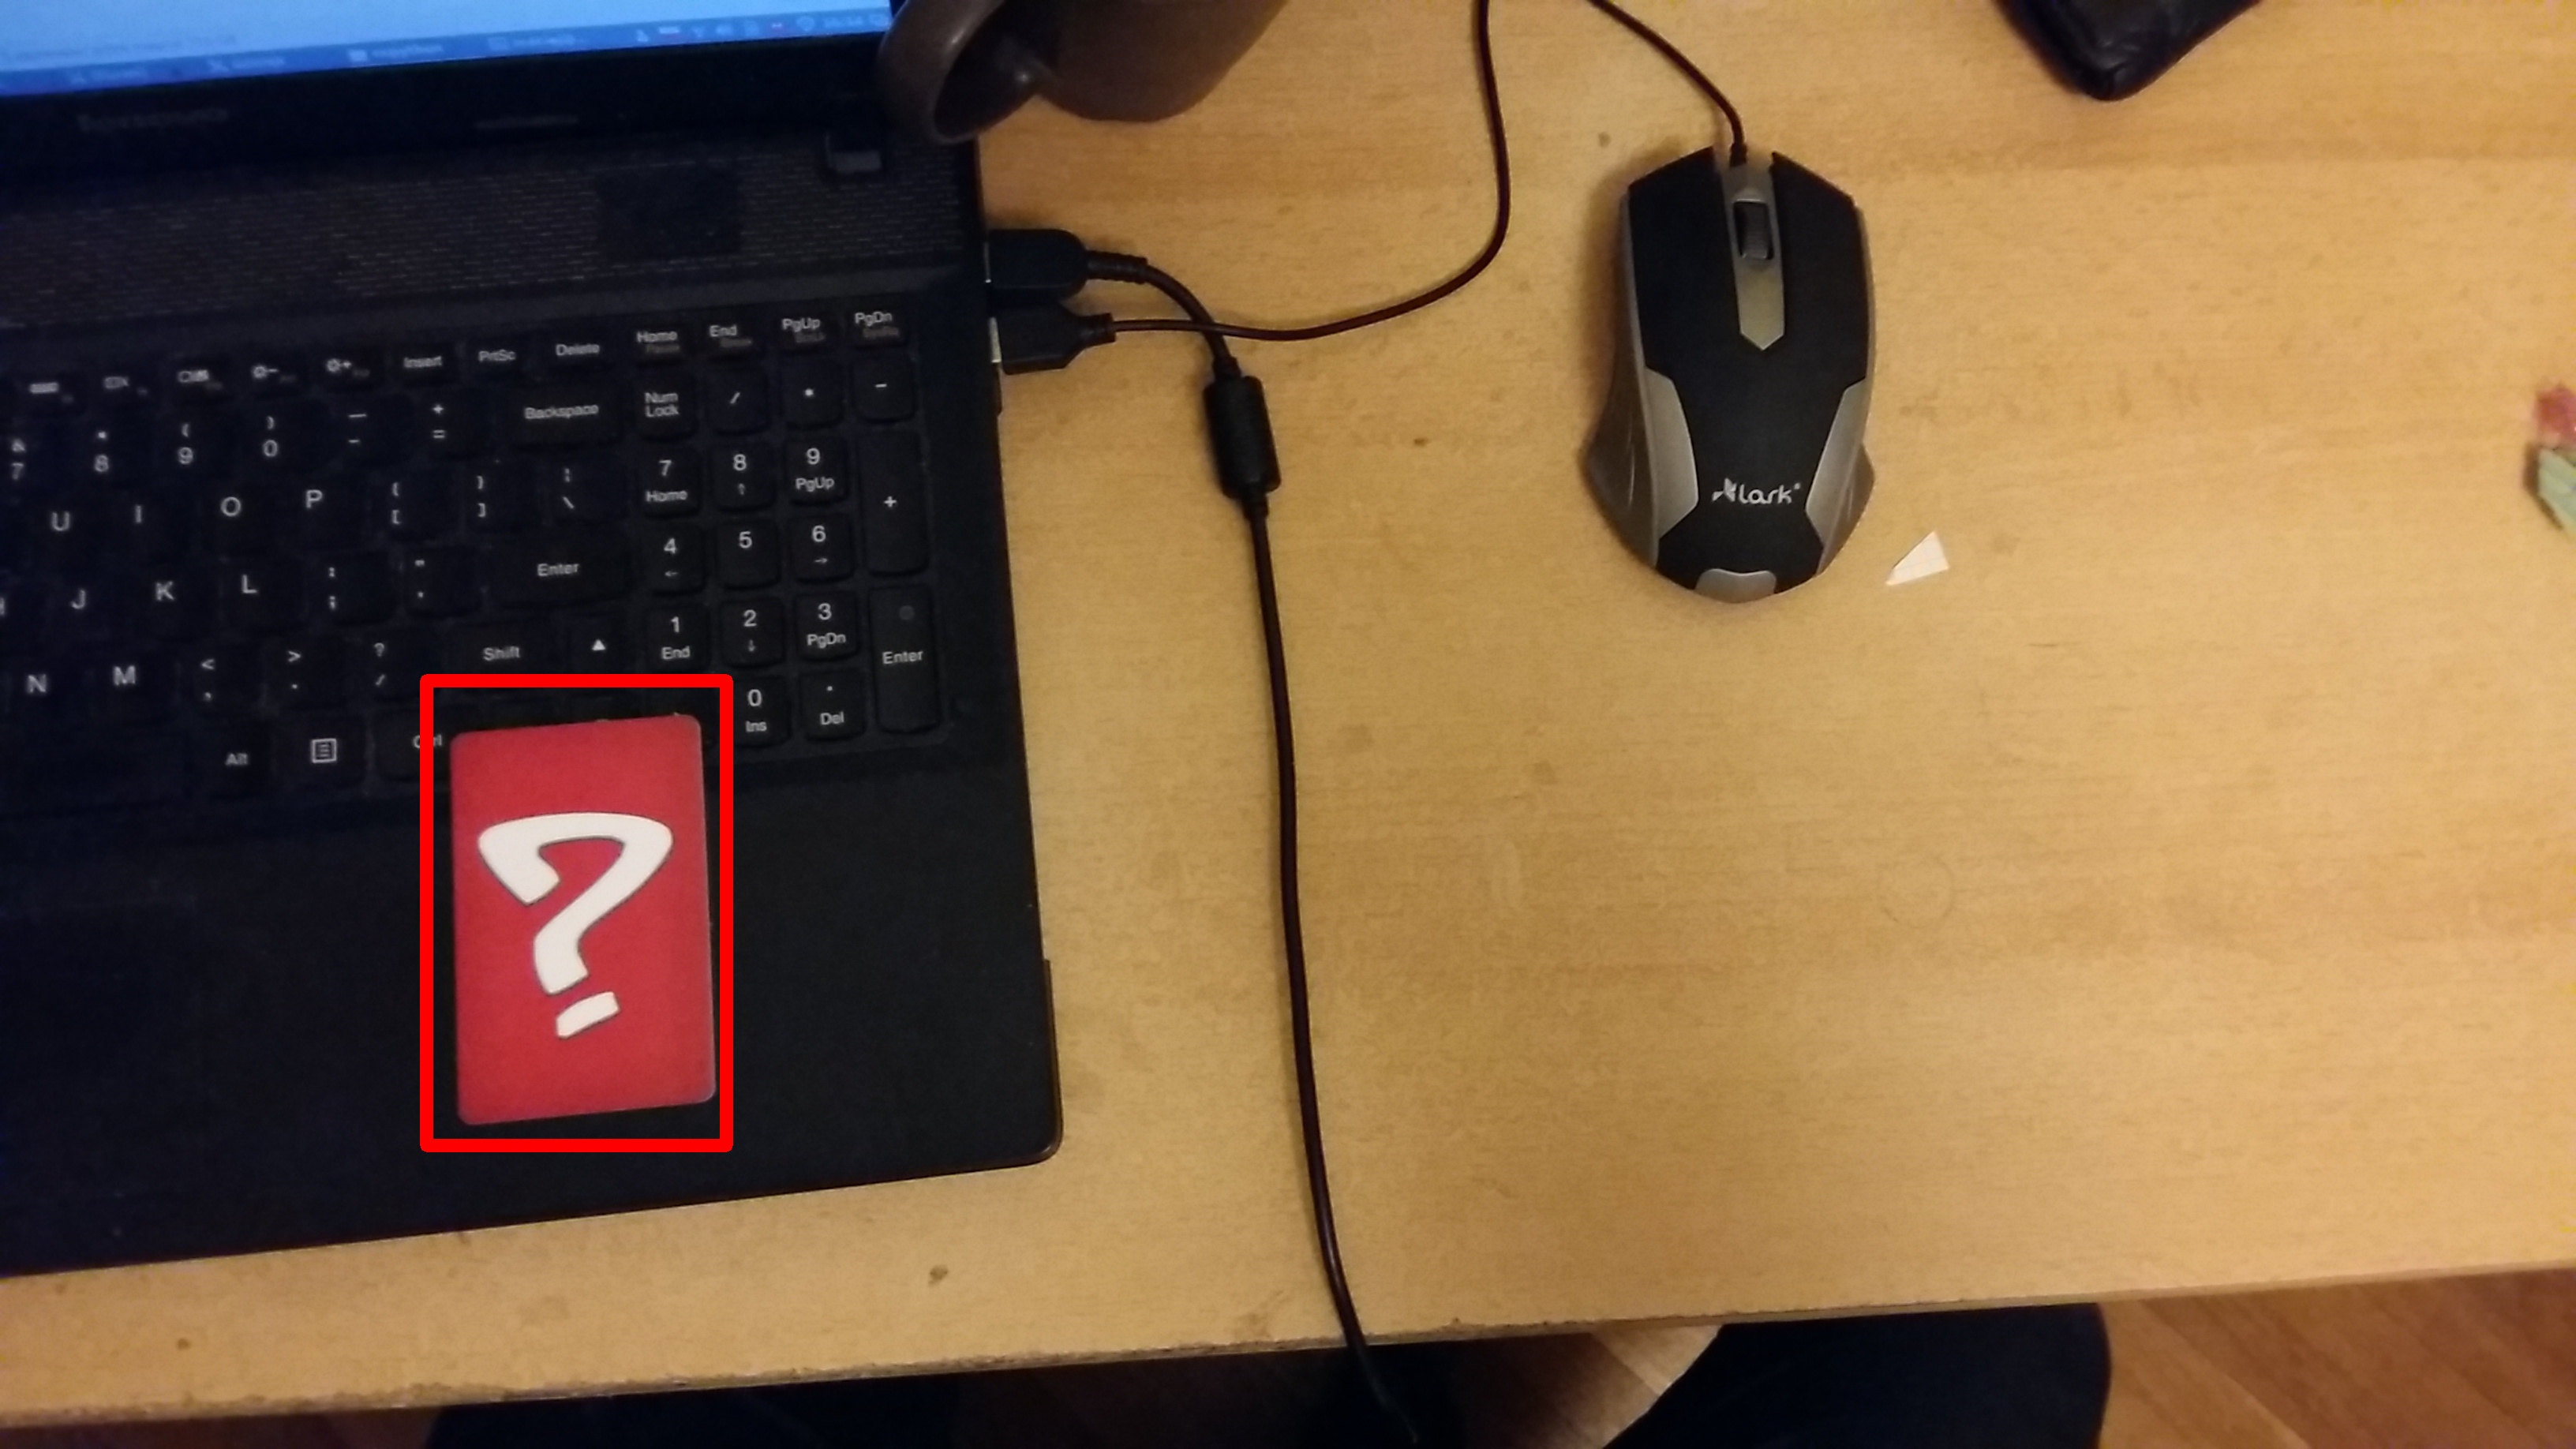
\includegraphics[width=\linewidth]{imgs/somsiadd16.jpg}
        \caption{minNeighbors równe 16}
        \label{fig:somsiadKarta16}
    \end{subfigure}
    \caption{Detekcja karty dla różnych wartości minNeighbors}
    \label{kartySomsiady}
\end{figure}


\begin{table}[H]
    \caption{Wyniki detekcji w zależności od parametru minNeighbors}
    \label{tab:somsiady}
    \begin{tabular}{|l|c|c|c|c|c|c|c|}
\hline
Rysunek & \ref{fig:somsiadTwarze1} & \ref{fig:somsiadTwarze3} & \ref{fig:somsiadTwarze8} & \ref{fig:somsiadKarta1} & \ref{fig:somsiadKarta6} & \ref{fig:somsiadKarta16}\\
\hline
Liczba sąsiadów & 1 & 3 & 8 & 1 & 6 & 16\\
\hline
Czas & 162,046 & 163,162 & 162,370 & 185,266 & 193,285 & 193,086\\
\hline
$F_{pos}$ & 2 & 0 & 0 & 28 & 4 & 0\\
\hline
$F_{neg}$ & 0 & 1 & 6 & 0 & 0 & 0\\
\hline
\end{tabular}
\end{table}

Rysunki \ref{twarzeeSomsiady} - \ref{kartySomsiady} przedstawiają wyniki detekcji twarzy oraz karty dla różnych parametrów minNeighbors. W tabeli \ref{tab:somsiady} przedstawiono rezultaty detekcji dla tych rysunków. Wynika z tego, że zmiana minimalnej liczby sąsiadów nie wpływa na czas detekcji. Przy zmianie parametru można jednak zauważyć dużą zmianę skuteczności. Dla wykrywania twarzy widać mniejszą liczbę ${F_{pos}}$ , stąd też dla mniejszej liczby minimalnych sąsiadów osiągnięto idealny rezultat.
W przypadku detekcji twarzy oraz oczu zdecydowano by zastosowano sugerowane wartości dla tych kaskad, są to:
\begin{itemize}
    \item minNeighbors = 3
    \item -scaleFactor = 1.3
\end{itemize}

Dla detekcji karty postanowiono przetestować dla jakich parametrów osiągnięto najlepszą skuteczność. W tym celu zebrano 10 zdjęć testowych na których znajduje się jedna karta. Na początku postanowiono ustawić parametr minNeighbors.
Zdjęcia przeszły proces detekcji, gdzie parametr minNeighbors przyjmował co drugą wartośc z zakresu <1,40> oraz scaleFactor równemu 1.3. Sprawdzano jaką liczbę odnalezionych obiektów. W przypadku wskazania jednego obiektu nie będącym szukaną kartą nie brano takiego pomiaru pod uwagę.

\begin{table}[H]
    \caption{Poszukiwanie najlepszej wartości minNeighbors cz. 1}
    \label{tab:somsiadyNaj1}
    \begin{tabular}{|c|c|c|c|c|c|c|c|c|c|c|}
\hline
minNeighbors & 1 & 3 & 5 & 7 & 9 & 11 & 13 & 15 & 17 & 19\\
\hline
Liczba odnalezionych & 11,62 & 6,89 & 4,89 & 3,68 & 3,03 & 2,86 & 2,51 & 1,89 & 1,68 & 1,82 \\
\hline
\end{tabular}
\end{table}

\begin{table}[H]
    \caption{Poszukiwanie najlepszej wartości minNeighbors cz. 2}
    \label{tab:somsiadyNaj2}
    \begin{tabular}{|c|c|c|c|c|c|c|c|c|c|c|}
\hline
minNeighbors & 21 & 23 & 25 & 27 & 29 & 31 & 33 & 35 & 37 & 39\\
\hline
Liczba odnalezionych &  1,34 & 1,20 & 1,06 & 0,91 & 0,75 & 0,65 & 0,48 & 0,44 & 0,41 & 0,34\\
\hline
\end{tabular}
\end{table}

W tabelach \ref{tab:somsiadyNaj1} i \ref{tab:somsiadyNaj2} przedstawiono średnie wartości liczby odnalezionych obiektów w zależności od parametru minNeighbors. Wynika z nich, że najlepsze decyzje były podejmowane dla wartości 25.
Na podstawie tego wyniku szukano najlepszej wartości parametru scaleFactor. Podobnie jak w poprzednim przypadku użyto tych samych dziesięciu zdjęć. Testowano wartości współczynnika scaleFactor od 1,1 do 1,7 co 0,05.

\begin{table}[H]
    \caption{Poszukiwanie najlepszej wartości scaleFactor}
    \label{tab:ckalaNaj}
    \begin{tabular}{|c|c|c|c|c|c|c|c|c|c|c|c|c|c|}
\hline
minNeighbors & 1.1 & 1.15 & 1.2 & 1.25 & 1.3 & 1.35 & 1.4 & 1.45 & 1.5 & 1.55 & 1.6 & 1.65 & 1.7\\
\hline
Liczba odnalezionych & 3,9 & 2,6 & 2,1 & 1,4 & 1,5 & 1,3 & 1,2 & 1,2 & 1,3 & 0,8 & 0,8 & 0,9& 0,8\\
\hline
\end{tabular}
\end{table}

W tabeli \ref{tab:ckalaNaj} przedstawiono średni wynik ilości odnalezionych obiektów w zależności od parametru scaleFactor. Dla detekcji karty w naszej aplikacji parametr ten będzie wynosił 1.4, ponieważ dla takiego parametru uzyskano najlepszą wartość będącą większą od 1, jednocześnie z pośród innych parametrów dla których uzyskano podobny wynik, ten gwarantuje mniejszą szansę przeoczenia obiektu.

\subsection{Zmniejszanie zdjęcia}
W przypadku naszej aplikacji wymaganie związane ze skutecznością ma większy priorytet niż czas działania. Dlatego pomyślano, że w przypadku kiedy nie zostanie podjęta jednoznaczna decyzja o odnalezieniu dokładnie jednego przedmiotu należy pomniejszyć zdjęcie i ponownie spróbować odnaleźć obiekt. Działanie takie podjęto ponieważ kaskada została wytrenowana na podstawie pomniejszonych zdjęć, więc powinna lepiej generalizować dla zdjęć pomniejszonych. W celu sprawdzenia tej teorii zebrano 10 zdjęć, dla których nie udało się wskazać dokładnie jednego obiektu, tak jak powinno zostać określone. Algorytm zakłada, że jeśli nie odnaleziono dokładnie jednego elementu, wysokosc i szerokosc zdjęcia dzielona jest przez 1,5. Następnie ponownie przeprowadzana jest detekcja obiektu. Proces ten się zakończy jeśli na którymś z etapów odnaleziono obiekt, lub szerokość osiągnie wartość minimalną, ustaloną na 120 pikseli. W rezultacie testu okazało się, że dla sześciu z dziesięciu zdjęć, w których przy oryginalnym rozmiarze wynik detekcji był niepoprawny, dla pomniejszonego zdjęcia udało się poprawnie odnaleźć obiekt. Operacja zmiany wielkości zdjęcia jest kosztowna jednak trwa znacznie krócej niż wykonanie ponownego zdjęcia i przeprowadzenie dla niego detekcji. Algorytm służący do testowania przeniesiono do kodu aplikacji co znacząco poprawiło skuteczność

\subsection{Wklejanie obrazu karty w miejsce obiektu}

Obrazy całej talii kart znajdują się zasobach aplikacji. Każdy z obrazów ma przypisane unikalne ID. Podczas wykonywania sztuczki, w momencie zbliżenia znacznika NFC z wiadomości zawartej w tagu odczytujemy ID przypisane do karty i zapisujemy w pamięci, tak by w trakcie wklejania wiadomym była która karta powinna zostać wklejona. 
W momencie kiedy detekcja obrazu jest zakończona zostaje wywołana procedura wklejania obrazu w miejsce wskazanego obiektu. W wyniku detekcji otrzymujemy współrzędne obiektu oraz jego szerokość i wysokość. Pierwszym etapem jest wczytanie obrazu karty z zasobów aplikacji. Następnie w zależności od wariantu jeśli wklejamy obraz na czoło potrzebujemy obrócić zdjęcie, ponieważ w zasobach jest zapisane w orientacji pionowej. Tak wczytany obraz karty następnie jest pomniejszany do rozmiarów odnalezionego obiektu. Kolejnym krokiem jest wyznaczenie w wykonanym zdjęciu obszaru obiektu, po czym w to miejsce jest kopiowana nasza przygotowana karta. Cały ten opis realizuje następująca funkcja.

\begin{lstlisting}[language=Java]
public void insertCardIntoImage(Mat img, Point lt, Point br) throws IOException {
        Mat card = Utils.loadResource(mainContext, resourceId, Imgcodecs.CV_LOAD_IMAGE_COLOR);
        if(br.x-lt.x> br.y-lt.y) {
            org.opencv.core.Core.flip(card.t(), card, 0);
        }
        Imgproc.resize(card, card, new Size((int)br.x - (int)lt.x, (int)br.y - (int)lt.y));
        Mat selectedArea = img.submat((int)lt.y, (int)br.y, (int)lt.x, (int)br.x);
        card.copyTo(selectedArea);
    }
\end{lstlisting}

\subsection{Implementacja w aplikacji}

W naszej aplikacji działania związane z wykonaniem zdjęcia oraz jego przetwarzania wykonują się z poziomu osobnej Aktywności.

\begin{figure}[H]
    \centering
        \begin{subfigure}{0.25\textwidth}
        \centering
        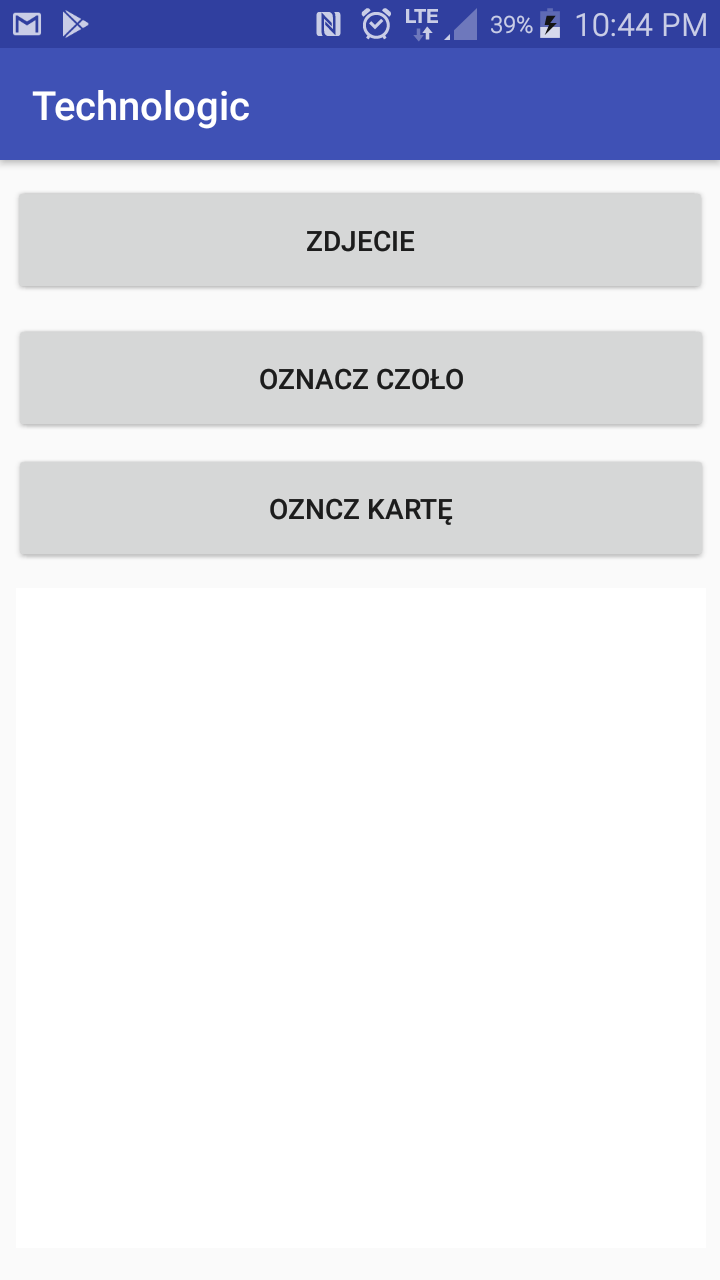
\includegraphics[width=\linewidth]{imgs/puste.png}
        \caption{po uruchomieniu}
        \label{fig:pustaAktywnosc}
    \end{subfigure}\hfill
    \begin{subfigure}{0.25\textwidth}
        \centering
        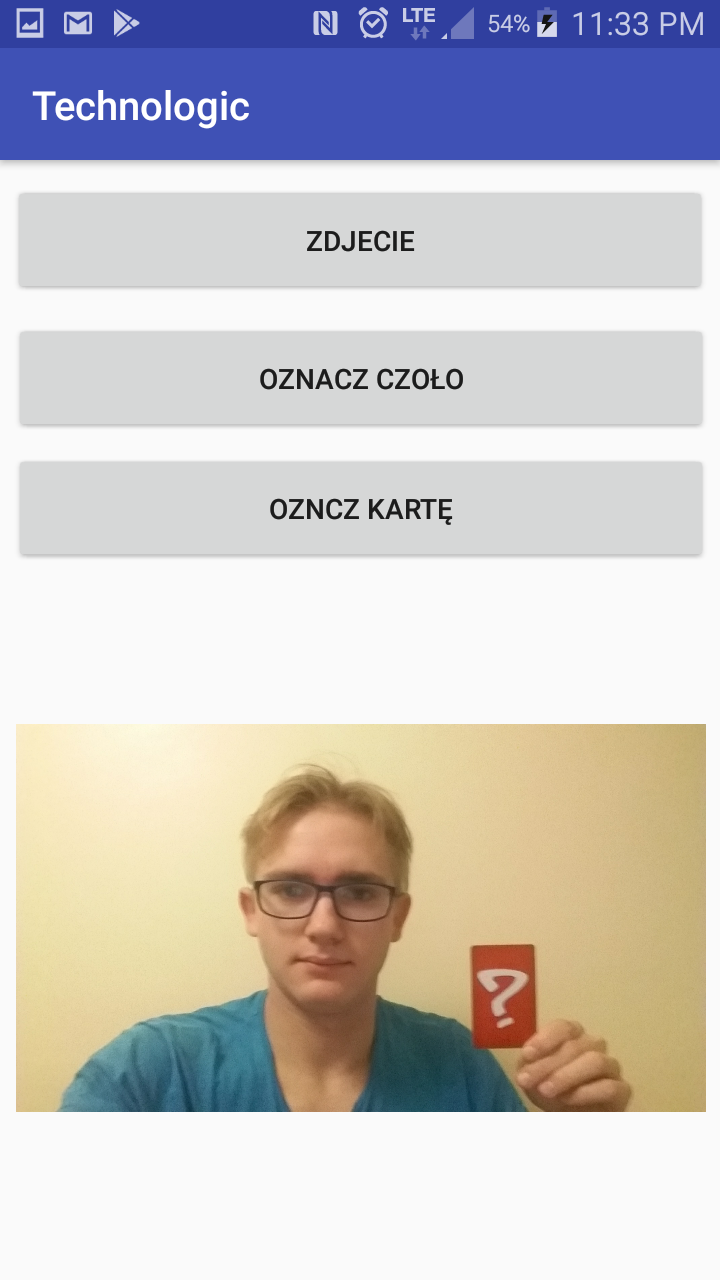
\includegraphics[width=\linewidth]{imgs/czyste.png}
        \caption{po wykonaniu zdjęcia}
        \label{fig:pusteZdjecie}
    \end{subfigure}\hfill
    \begin{subfigure}{0.25\textwidth}
        \centering
        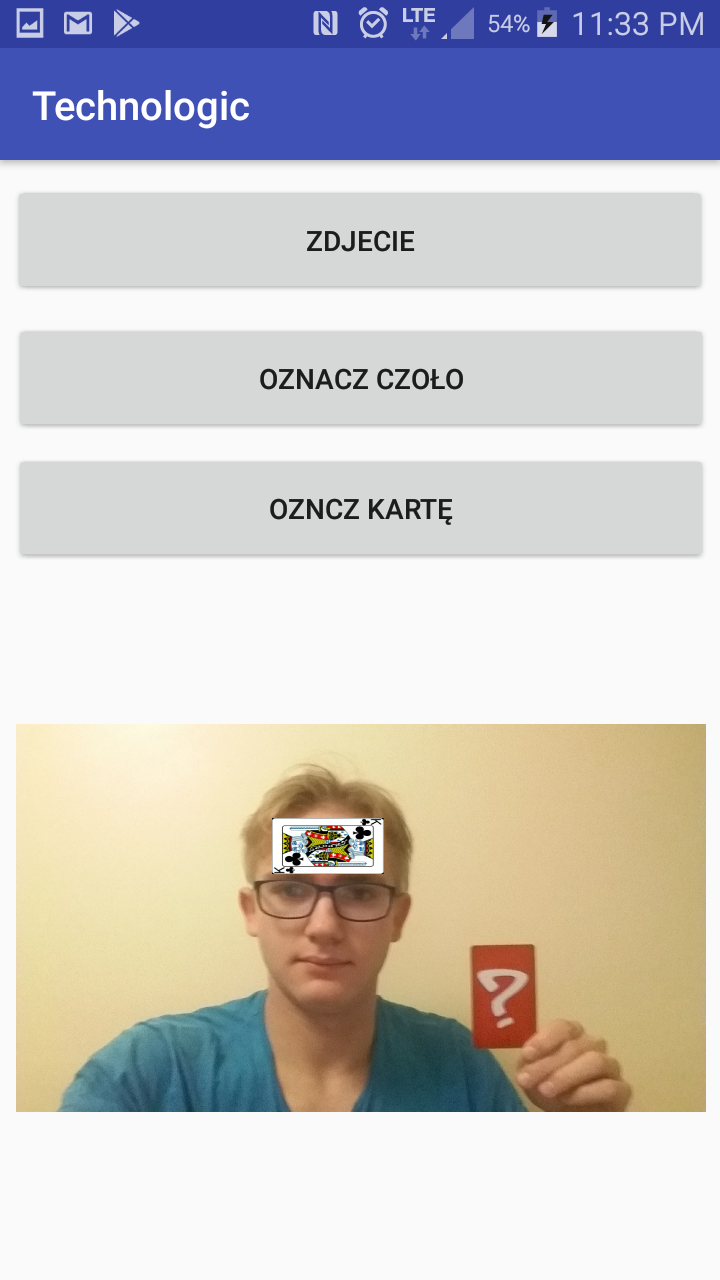
\includegraphics[width=\linewidth]{imgs/czolo.png}
        \caption{po detekcji czoła}
        \label{fig:zdjecieCzolo}
    \end{subfigure}\hfill
    \begin{subfigure}{0.25\textwidth}
        \centering
        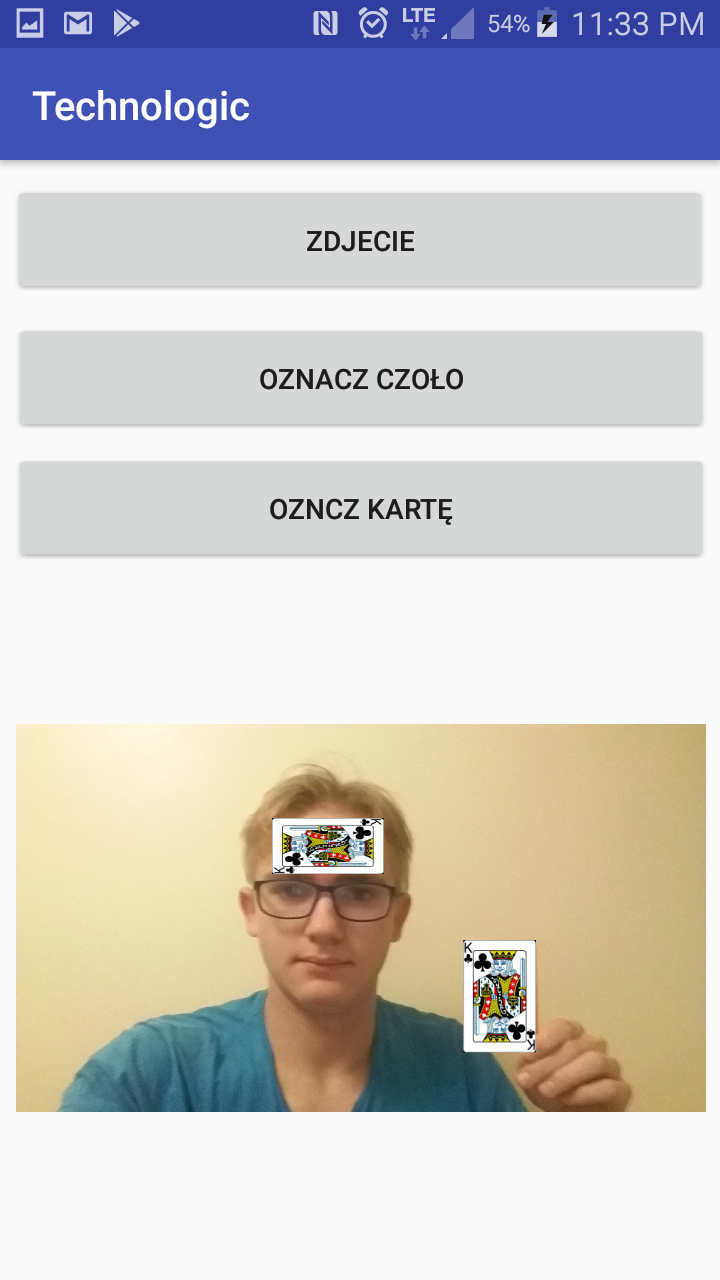
\includegraphics[width=\linewidth]{imgs/oba.png}
        \caption{po detekcji karty}
        \label{fig:zdjecieObo}
    \end{subfigure}
    \caption{Widoki aktywności obsługującej zdjęcia}
    \label{widokiPhoto}
\end{figure}

Rysunek \ref{widokiPhoto} przedstawia widok Aktywności w której realizowane są operacje związane ze zdjęciem. Widok aktywności składa się z trzech przycisków oraz okienka z obrazkiem. 
Po wciśnięciu przycisku z napisem ZDJĘCIE zostaje uruchomiona systemowa aplikacja aparatu, która po wykonaniu zdjęcia prosi o zatwierdzenie wykonanego zdjęcia. Jeśli zaakceptowano zdjęcie następuje automatyczny powrót do naszej aplikacji.
Po stronie naszej aplikacji kod wygląda następująco:

\begin{lstlisting}[language=Java]
public void takePic(){
    pictureFile = getPictureFile();
    Intent intent = new Intent(MediaStore.ACTION_IMAGE_CAPTURE);
    intent.putExtra(MediaStore.EXTRA_OUTPUT, Uri.fromFile(getPictureFile()));
    //pathPic = dest.getPath();        ((Activity)mainContext).startActivityForResult(intent, REQUEST_IMAGE);
}
@Override
protected void onActivityResult(int requestCode, int resultCode, Intent data) {
    if( requestCode == pictureService.REQUEST_IMAGE && resultCode == Activity.RESULT_OK ){
        pictureService.updateImage();
    }
}
\end{lstlisting}

Po wykonaniu zdjęcia w okienku pojawia się wykonane zdjęcie tak jak na rysunku \ref{fig:pusteZdjecie}. Następnie w zależności od wariantu sztuczki można wybrać przycisk OZNACZ CZOŁO albo OZNACZ KARTĘ. W przypadku pierwszego uruchamiamy następującą funkcję, która naniesie obraz karty w miejsce odnalezienia czoła:

\begin{lstlisting}[language=Java]
public Mat picToMark(Mat aInputFrame) throws IOException {
    Imgproc.cvtColor(aInputFrame, grayscaleImage, Imgproc.COLOR_RGBA2RGB);
    ObjectReconizer fR=new ObjectReconizer(mainContext, R.raw.lbpcascade_frontalface, mainContext.getString(R.string.cascadeFrontalFaceXML), grayscaleImage, 1.3, 3);
    MatOfRect faces=fR.getObjects();
    org.opencv.core.Rect[] facesArray = faces.toArray();
    if(facesArray.length>0) {
        ObjectReconizer eR=new ObjectReconizer(mainContext, R.raw.haarcascade_lefteye_2splits, "haarcascade_lefteye_2splits.xml", grayscaleImage, 1.3, 3);
        for (int i = 0; i < facesArray.length; i++) {
            org.opencv.core.Rect face=facesArray[i];
            org.opencv.core.Rect abcd =new org.opencv.core.Rect(face.x, face.y, face.width, face.height);
            Mat roi_color= new Mat(aInputFrame, abcd);
            eR.setGrayScaleImage(roi_color);
            MatOfRect eyes=eR.getObjects();
            org.opencv.core.Rect[] eyesArray=eyes.toArray();
            if(eyesArray.length==2){
                int x=(eyesArray[0].x<eyesArray[1].x) ? eyesArray[0].x:eyesArray[1].x;
                int x2=(eyesArray[0].x>eyesArray[1].x) ? eyesArray[0].x+eyesArray[0].width:eyesArray[1].x+eyesArray[1].width;
                int y = eyesArray[0].y;
                int w=x2-x;
                int h=w/2;
                insertCardIntoImage(roi_color, new Point(0, x), new Point(h, w+x));
            }
        }
    }
    return aInputFrame;
}
\end{lstlisting}

Po wykonaniu tej operacji w miejsce odnalezienia czoła zostanie wklejony obraz karty, tak jak na rysunku \ref{fig:zdjecieCzolo}. 
Jeśli wybrany jest wariant by karta została wklejona w miejsce naszego znaku zapytania wybieramy przycisk OZNACZ KARTĘ w tym wypadku uruchomi się następująca funkcja:

\begin{lstlisting}[language=Java]
public void markCard() throws IOException {
    if(grayscaleImage==null)grayscaleImage=new Mat();
    Mat pictureToMark= Imgcodecs.imread(pictureFile.getPath());
    double width=pictureToMark.size().width;
    double height=pictureToMark.size().height;
    MatOfRect cards = new MatOfRect();
    while(width>120.0){
        Imgproc.cvtColor(pictureToMark, grayscaleImage, Imgproc.COLOR_RGBA2RGB);
        ObjectReconizer cR=new ObjectReconizer(mainContext, R.raw.newcard, "newcard.xml", grayscaleImage, 1.4, 25);
        cards=cR.getObjects();
        if(cards.toArray().length!=1){
            width/=1.5;
            height/=1.5;
            Imgproc.resize(pictureToMark, pictureToMark, new Size(width,height ));
        }
        else break;
    }
    org.opencv.core.Rect[] cardsArray = cards.toArray();
    if(cardsArray.length==1){
        Mat picToMarkAfterResize = Imgcodecs.imread(pictureFile.getPath());
        double ratio= picToMarkAfterResize.size().width/width;
        Point lt=new Point(cardsArray[0].tl().x*ratio, cardsArray[0].tl().y*ratio);
        Point br=new Point(cardsArray[0].br().x*ratio, cardsArray[0].br().y*ratio);
        insertCardIntoImage(picToMarkAfterResize, lt, br);
        pictureToMark=picToMarkAfterResize;
    }
    pictureFile = getPictureFile();
    Imgcodecs.imwrite(pictureFile.getPath(), pictureToMark);
    updateImage();
}
\end{lstlisting}

Po wykonaniu tej operacji karta została wklejona w miejsce odnalezionego obiektu. Rysunek \ref{fig:zdjecieObo} przedstawia widok po wykonaniu detekcji karty po wcześniejszej detekcji czoła.
 \newpage
\section{Technologia NFC}
NFC (ang. Near Field Communication) to w dosłownym tłumaczeniu komunikacja bliskiego zasięgu. Polega ona na bezprzewodowej technologii krótkiego zasięgu. Tag NFC to pasywne urządzenie NFC, zasilane polem NFC urządzenia, gdy znajduje się ono w zasięgu. Wyróżnia się cztery rodzaje tagów, różnią się od siebie pojemnością i/lub formatem.  Zazwyczaj wymagają odległości 4cm lub mniejszej, aby zainicjować połączenie.  Tagi mogą mieć różną złożoność. Proste znaczniki oferują tylko możliwość odczytu i zapisu, czasem z programowalnym obszarem infromującym, że zawartość jest tylko do odczytu. Bardziej skomplikowane tagi oferują operacje matematyczne i mają sprzęt kryptograficzny do uwierzytelniania. Najbardziej wyrafinowane tagi zawierają środowisko operacyjne, pozwalające na złożone interakcje z kodem wykonującym na tagu.
\paragraph{Zasada działania}\mbox{}\\
NFC opiera się na efekcie indukcji elektromagnetycznej. Gdy znacznik znajdzie się obrębie pola magnetycznego, generowana jest energia elektryczna. Sygnał przepływa między dwiema antenami – w smartfonie i w sprzęcie docelowym (również może to być smartfon). W ten sposób zestabilizowane zostaje połączenie zapewniające komunikację między urządzeniami za pomocą fal radiowych krótkiego zasięgu.
\subsection{Historia NFC}
Pierwsze próby z tą technologią rozpoczęto jeszcze na początku lat 80. W 1983 r. złożono wówczas pierwszy patent związaniu z technologią RFID (ang. Radio-frequency identification), która jest inspiracją dla NFC. Dopiero w 2004 roku została utworzona organizacja mająca na celu rozwój technologii NFC - NFC Forum.
\par
Trzeba było kolejnych lat, by dopiero w 2009 r. zostały opracowane kolejne elementy układanki, która pozwoliła na wygodne korzystanie z NFC. Dopiero siedem lat temu zaczęły działać pierwsze standardy przesyłania zarówno kontaktów czy adresów URL. W tym samym czasie stworzono również sposób na inicjalizację nadajnika Bluetooth. Dzięki temu nie trzeba korzystać z niezbyt wygodnego parowania urządzeń. Zamiast tego wystarczy zbliżyć do siebie czytnik (smartfon) z kartą NFC (głośnik bezprzewodowy) by nawiązać między nimi łączność Bluetooth.
\subsection{NFC na platforie Android}
Funkcja NFC umożliwia udostępnianie niewielkich ładunków danych między tagiem NFC, a urządzeniem z systemem Android lub między dwoma urządzeniami. Dane przechowywane w tagu mogą być również zapisane w różnych formatach, ale wiele interfejsów API systemu Android jest opartych na standardzie NFC Forum o nazwie Ndef. Urządzenia z systemem Android z obsługą NFC realizują jednocześnie trzy główne tryby działania:
\begin{itemize}
\item Tryb czytnika/zapisywacza - umożliwia urządzeniu NFC odczytywanie i/lub zapisywanie pasywnych tagów NFC i naklejek.
\item Tryb peer-to-peer - umożliwia urządzeniu NFC wymianę danych z innym urządzeniem NFC. Korzysta z niego funkcja Android Beam.
\item Tryb emulacji kart - umożliwia urządzeniu NFC działać jak karta NFC. Dostęp do emulowanej karty NFC można uzyskać za pomocą zewnętrznego czytnika np. terminalu płatniczego NFC.
\end{itemize}
 Funkcja Android Beam umożliwia urządzeniu przesyłanie wiadomości NDEF na inne urządzenie poprzez fizyczne dotykanie urządzeń. Ta interakcja zapewnia łatwiejszy sposób wysyłania danych niż inne technologie bezprzewodowe, takie jak Bluetooth, ponieważ w przypadku NFC nie jest wymagane ręczne wykrywanie urządzeń ani parowanie. Połączenie zostanie automatycznie uruchomione, gdy dwa urządzenia znajdą się w zasięgu.
\subsubsection{NfcAdapter}
Reprezentuje lokalny moduł NFC. Posiada trzy stałe określające akcję dla Intencji:
\begin{itemize}
    \item \textit{ACTION\_TAG\_DISCOVERED} - dowolny tag NFC został wykryty
    \item \textit{ACTION\_NDEF\_DISCOVERED} - został wykryty tag z danymi NDEF
    \item \textit{ACTION\_TECH\_DISCOVERED} - został wykryty tag, którego technologia została zarejestrowana w jakieś Aktywności
\end{itemize}
Tworzenie nowego obiektu zawierającego strukturę NfcAdapter sprowadza się do wywołania statyczej metody tej klasy \textit{getDefaultAdapter(context)}. Poniżej przedstawiony jest konstruktor zaimplementowanej przez nas klasy NfcService. 
\begin{lstlisting}[language=Java]
public NfcService(Context context){
        this.context = context;
        this.nfcAdapter = NfcAdapter.getDefaultAdapter(context);
}
\end{lstlisting}
W parametrze \textit{context} przekazywany jest obiekt Aktywności, która korzysta z NFC. Dodatkowo, aby nasza Aktywność miała pierwszeństwo do obsłużenia wykrytego tagu, gdy jest na pierwszym planie, musimy nadpisać jej metodę onResume(). W ciele tej metody musi występować wywołanie funkcji klasy NfcAdapter \textit{enableForegroundDispatch (Activity activity, PendingIntent intent, IntentFilter[] filters, String[][] techLists)}. Jeśli został podany parametr \textit{filters}, jest ona używany do dopasowania Intencji wysyłanych zarówno dla \textit{ACTION\_NDEF\_DISCOVERED}, jak i \textit{ACTION\_TAG\_DISCOVERED}. Ponieważ \textit{ACTION\_TECH\_DISCOVERED} opiera się na metadanych zawartych w tagu, jego dopasowanie jest obsługiwane przez osobną listę zarejestrowanych technologii w parametrze \textit{techLists}. Jeśli parametry \textit{filters} i \textit{techList} będą \textit{null} to wszystkie wykryte znaczniki zostanę przekazane do Aktywności na pierwszym planie. W naszej klasie klasie NfcService, zostało to zrealizowane w postaci publicznej metody, która może zostać wywołana z poziomu Aktywności, gdzie został utworzony obiekt klasy NfcService.
\begin{lstlisting}[language=Java]
public void enableForegroundDispatchSystem(){
    Intent intent = new Intent(context, context.getClass());
    intent.addFlags(Intent.FLAG_RECEIVER_REPLACE_PENDING);
    Intent[] intentArray = new Intent[]{intent};
    PendingIntent pending = PendingIntent.getActivities(context, 0, intentArray, 0);
    IntentFilter[] filters = new IntentFilter[] {};
    nfcAdapter.enableForegroundDispatch((Activity)context, pending, filters, null);
}
\end{lstlisting}
Gdy Aktywność obługująca wykryte tagi NFC zniknie z pierwszego planu, należy niezwłocznie wyłączyć jej tę możliwość. Najlepiej zrobić to w nadpisanej metodzie \textit{onPause()} Aktywności korzystającej z NFC. 
\begin{lstlisting}[language=Java]
public void disableForegroundDispatchSystem(){
        nfcAdapter.disableForegroundDispatch((Activity)context);
}
\end{lstlisting}
\subsubsection{Znacznik}
Znacznik (ang. Tag) jest to niezmienny obiekt rezprezentujący stan znacznika NFC w momencie wykrycia. Może być używany jako uchwyt, aby wykonywać bardziej zaawansowane operacje. Nowy obiekt Znacznika jest tworzony za każdym razem, gdy moduł NFC go wykryje. Nie ma znaczenia czy jest to fizycznie ten sam znacznik. Uzyskanie obiektu Znacznika jest możliwe poprzez wyciągnięcie go z obiektu Intencji przekazanego do Aktywności pierwszego planu. Dlatego tak ważne jest uruchamianie metody enableForegroundDispatch(), w metodzie onResume() Aktywności. 
\begin{lstlisting}[language=Java]
public boolean setNfcTag(Intent intent) {
        if(intent.hasExtra(NfcAdapter.EXTRA_TAG)){
            tag = getTag(intent);
            return true;
        }
        return false;
}
private Tag getTag(Intent intent) {
        return intent.getParcelableExtra(NfcAdapter.EXTRA_TAG);
}
\end{lstlisting}
Metoda \textit{setNfcTag()} jest wywoływana w nadpisanej metodzie \textit{onNewIntent()} Aktywności, która obsługuje żądanie NFC.
\subsubsection{Zapis i odczyt danych z użyciem tagu NFC}

Ndef (ang. NFC Data Exchenge Format) to lekki format binarny, używany do enkapsulacji wpisanych danych. Jest określony przez NFC Forum do transmisji i przechowywania danych za pomocą NFC. Obiekt tej klasy uzyskuje się za pomocą statycznej metody klasy Ndef \textit{get(Tag tag)}. Zawiera w sobie Wiadomości (ang. NdefMessages) i Rekordy (ang. NdefRecords). Rekordy zawierają w sobie dane, może to być nośnik MIME, URI lub niestandardowe dane aplikacji. Natomiast Wiadomości są zbiorem Rekordów.
\paragraph{Zapis}\mbox{}\\
Zapis danych do tagu polega na poprawnym przygotowaniu Rekordu Ndef. Stworzeniu na jego podstawie Wiadomości Ndef, a następnie nadpisaniu poprzedniej Wiadomości Ndef w znaczniku (o ile znacznik nie jest tylko do odczytu).
\begin{lstlisting}[language=Java]
public boolean writeToNfcTag(String content){
        return writeNdefMessage(content);
}

private NdefMessage createNdefMessage(String content){
    NdefRecord record = NdefRecord.createTextRecord(null, content);
    return new NdefMessage(record);
}

private boolean writeNdefMessage( String content){
    try{
        if(tag == null){
            return false;
        }
        else{
            Ndef ndef = Ndef.get(tag);
            NdefMessage mess = createNdefMessage(content);
            if(ndef == null){
                return false;
            }
            else{
                ndef.connect();
                if(!ndef.isWritable()){
                    ndef.close();
                    return false;
                }
                ndef.writeNdefMessage(mess);
                ndef.close();
                return true;
            }
        }
    }
    catch(Exception e){
        return false;
    }
}
\end{lstlisting}
Efektem graficznym tego fragmentu jest następująca Aktywność. Wyświetlony Toast został wywołany po zbliżeniu znacznika do smartfonu i poprawnym zapisie danych do niego.
\begin{figure}[H]
    \centering
    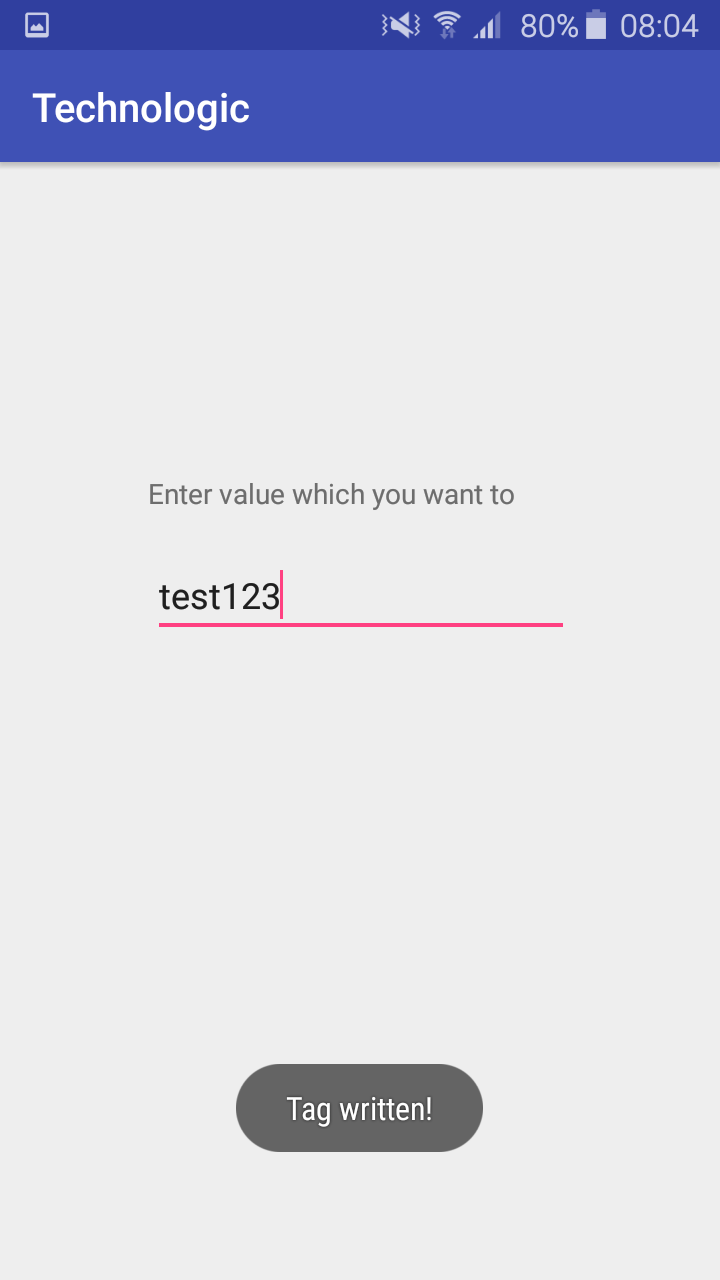
\includegraphics[scale=0.22]{imgs/write.png}
    \caption{Aktywność do zapisywania danych do tagu NFC}
\end{figure}
\paragraph{Odczyt}\mbox{}\\
Odczyt danych Ndef z tagu NFC jest obsługiwany za pomocą systemu rozsyłania tagów, który analizuje wykryte znaczniki NFC, odpowiednio kategoryzuje dane i uruchamia aplikację, która jest zainteresowana skategoryzowanymi danymi. Aplikacja, która chce obsłużyć zeskanowany tag NFC, może zadeklarować filtr intencji i żądanie obsługi danych.
\begin{lstlisting}[language=Java]
public String readFromNfcTag(){
        return readTextFromTag();
}

private String readTextFromTag() {
    Ndef ndef = Ndef.get(tag);
    if(ndef == null) return null;
    NdefMessage ndefMessage;
    try {
        ndef.connect();
        ndefMessage = ndef.getNdefMessage();
    }
    catch(Exception ex){
        return null;
    }
    NdefRecord[] records = ndefMessage.getRecords();
    if(records != null && records.length > 0){
        NdefRecord record = records[0];
        return getTextFromNdefRecord(record);
    }
    return null;
}

private String getTextFromNdefRecord(NdefRecord record) {
    String tagContent = null;
    try{
        byte[] payload = record.getPayload();
        String textEncoding = "UTF-8";
        int languageSize = payload[0] & 0063;
        tagContent = new String(payload, languageSize + 1,
                payload.length - languageSize - 1, textEncoding);

    } catch (UnsupportedEncodingException e) {
        e.printStackTrace();
    }
    return tagContent;
}
\end{lstlisting}
Efekt graficzny tego fragmentu przedstawia się następująco. Jest to sytuacja, gdy zbliżony tag został poprawnie odczytany. Jednocześnie, jeśli był dla danego tagu (karty) określony schemat wibracji, zostaje on wywibrowany.
\begin{figure}[H]
    \centering
    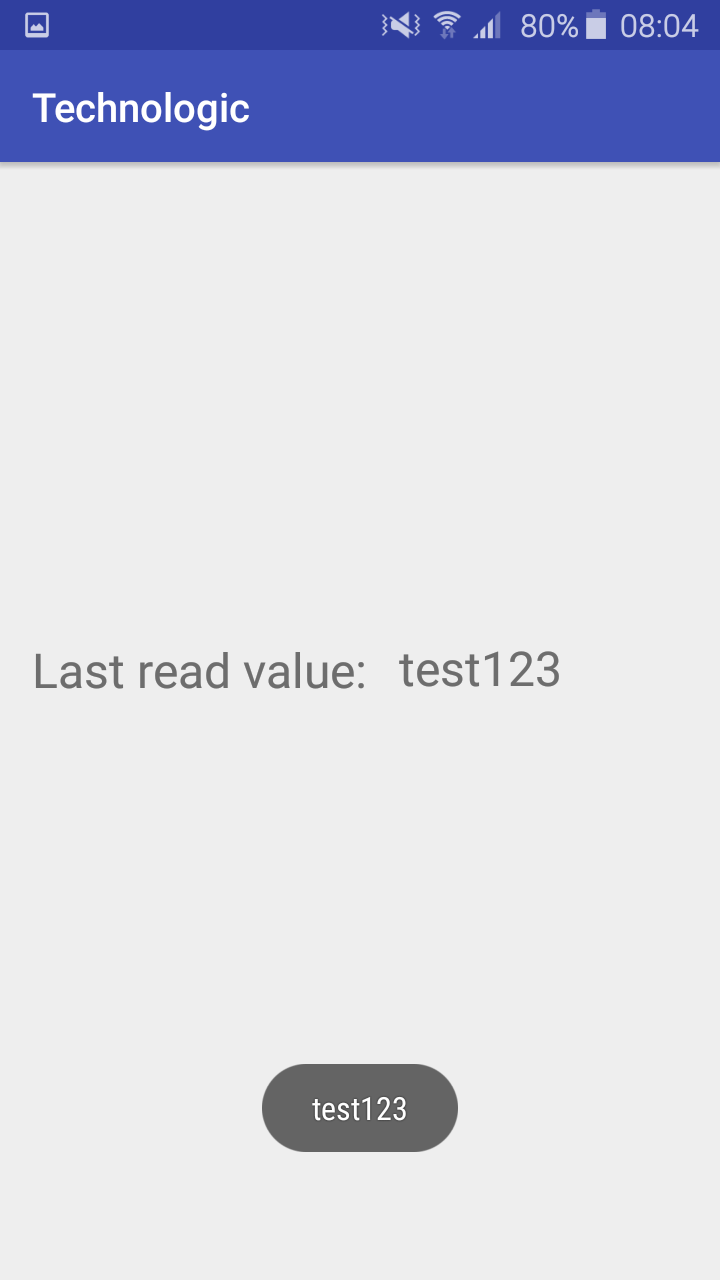
\includegraphics[scale=0.22]{imgs/read.png}
    \caption{Aktywność do odczytywania danych do tagu NFC}
\end{figure}
 \newpage
\section{Podsumowanie}
Zrealizowany projekt miał na celu opracowania aplikacji mobilnej, umożliwiającej wykonanie sztuczki karcianej. Wynikiem pracy jest działający program możliwy do uruchomienia na telefonach z systemem Android w wersji 5.0+. W realizacji celu wykorzystano wbudowane komponenty telefonu takie jak aparat, wibrator oraz moduł NFC. Dodatkowo wytworzono własne kaskady klasyfikatorów zdolnych do rozpoznawania obiektów. Zrealizowano obsługę aparatu z poziomu aplikacji, możliwość odczytu i zapisu wiadomości do znaczników NFC, wykorzystanie wibratora do wibrowania w zdefiniowanych przez nas odstępach czasu, detekcję obiektów na wykonanym zdjęciu oraz wytrenowaną własną kaskadę Haar'a.
Dodatkowo można wskazać kilka funkcji, które usprawniłyby naszą aplikację lub rozszerzyły by jej funkcjonalność:
\begin{itemize}
    \item Zastosowanie innych sposobów detekcji, np. przy użyciu splotowych sieci neuronowych.
    \item Umożliwienie wysyłania wykonanego zdjęcia przy użyciu poczty elektronicznej
    \item Zastosowanie wstępnej detekcji w czasie rzeczywistym podczas wykonywania zdjęcia.
    \item Dodanie samouczka, który wyjaśniał by w jaki sposób używać aplikacji
    \item Umieszczenie aplikacji w Sklepie Play
\end{itemize}
 \newpage

\renewcommand{\baselinestretch}{1.0}\normalsize	% żeby w wykazach była pojedyncza interlinia

\addcontentsline{toc}{section}{Wykaz literatury}
\nocite{*}
\printbibliography
\newpage
\addcontentsline{toc}{section}{\listfigurename}
\listoffigures
\newpage

\addcontentsline{toc}{section}{\listtablename}
\listoftables

\renewcommand{\baselinestretch}{1.5}\normalsize	% powrót do interlinii 1.5 na wypadek dodatków

% nie dodawaj obrazków i tabel z dodatków do list powyżej
\let\svaddcontentsline\addcontentsline
\renewcommand\addcontentsline[3]{%
  \ifthenelse{\equal{#1}{lof}}{}%
  {\ifthenelse{\equal{#1}{lot}}{}{\svaddcontentsline{#1}{#2}{#3}}}}

\newpage

\begin{appendices}
\addtocontents{toc}{\protect\setcounter{tocdepth}{1}}

\section{Przykładowy dodatek} \label{app:example}

\subsection{Sekcja}
\lipsum[40]
 \newpage
\end{appendices}

\end{document}	% musi być na samiutkim końcu
